\documentclass{beamer}
\usetheme{}
\usecolortheme{dolphin}           
\useinnertheme{circles}
\setbeamertemplate{itemize items}[default]
\setbeamertemplate{enumerate items}[default]
\usepackage[T1]{fontenc}
\usepackage[utf8]{inputenc}
\usepackage{lmodern}
\usepackage{amsmath}
\usepackage{booktabs} 
\usepackage{graphicx}        
\usepackage{array}
\usepackage{color}
\makeatletter
\def\zapcolorreset{\let\reset@color\relax\ignorespaces}
\def\colorrows#1{\noalign{\aftergroup\zapcolorreset#1}\ignorespaces}
\makeatother
\graphicspath{{/home/swl/Dropbox/ucd/advanced_macro/figures/}} 
\setbeamertemplate{navigation symbols}{}

%--------------------------------------
\title{Time-series data}
\author{School of Economics, University College Dublin}
\date{Spring 2018}
\begin{document}

%--------------------------------------
\begin{frame}
 \titlepage
\end{frame}
%--------------------------------------

%--------------------------------------
\begin{frame}
 Things to do in empirical macroeconomics:
  \begin{enumerate}
  \item Data description: Describe and summarize macroeconomic data 
  \item Forecasting: Make macroeconomic forecasts 
  \item Structural inference: Quantify what we know and don't know about the true structure of the macro economy 
  \item Policy analysis: Advise on macroeconomic policy 
  \end{enumerate}
\end{frame}
%--------------------------------------

%--------------------------------------
\begin{frame}
  \begin{figure}
    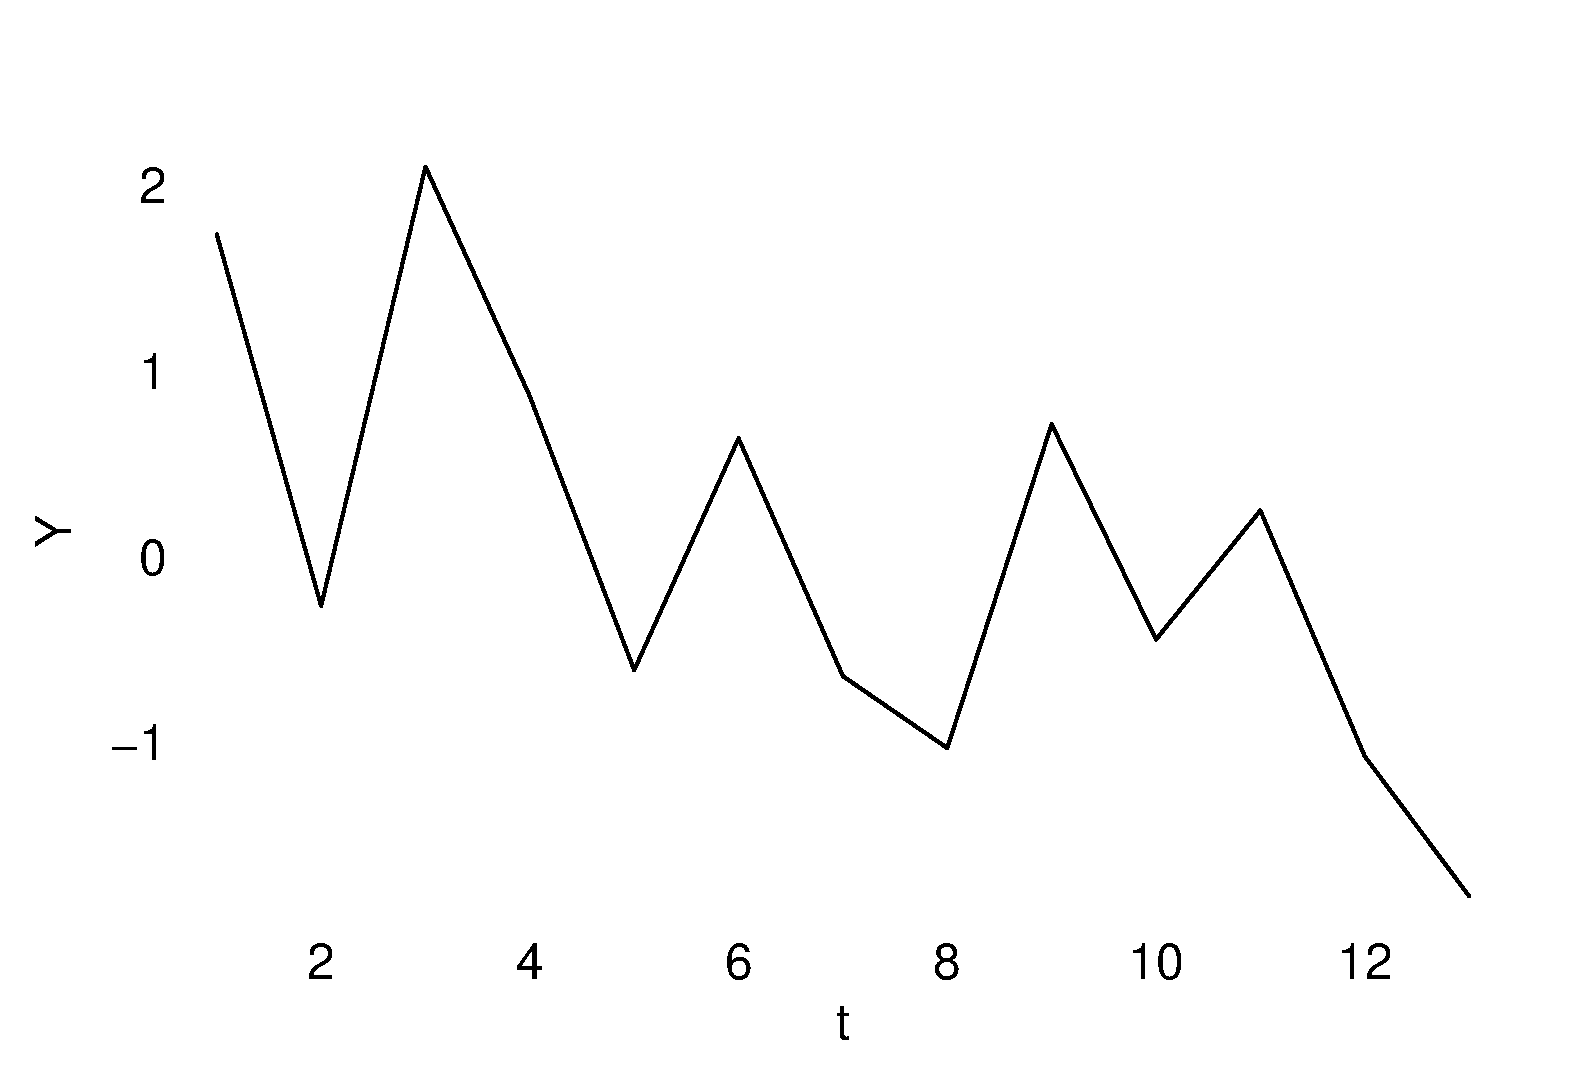
\includegraphics[scale=.4]{ts_example.eps}
  \end{figure}
\end{frame}
%--------------------------------------

%--------------------------------------
\begin{frame}
  \begin{figure}
    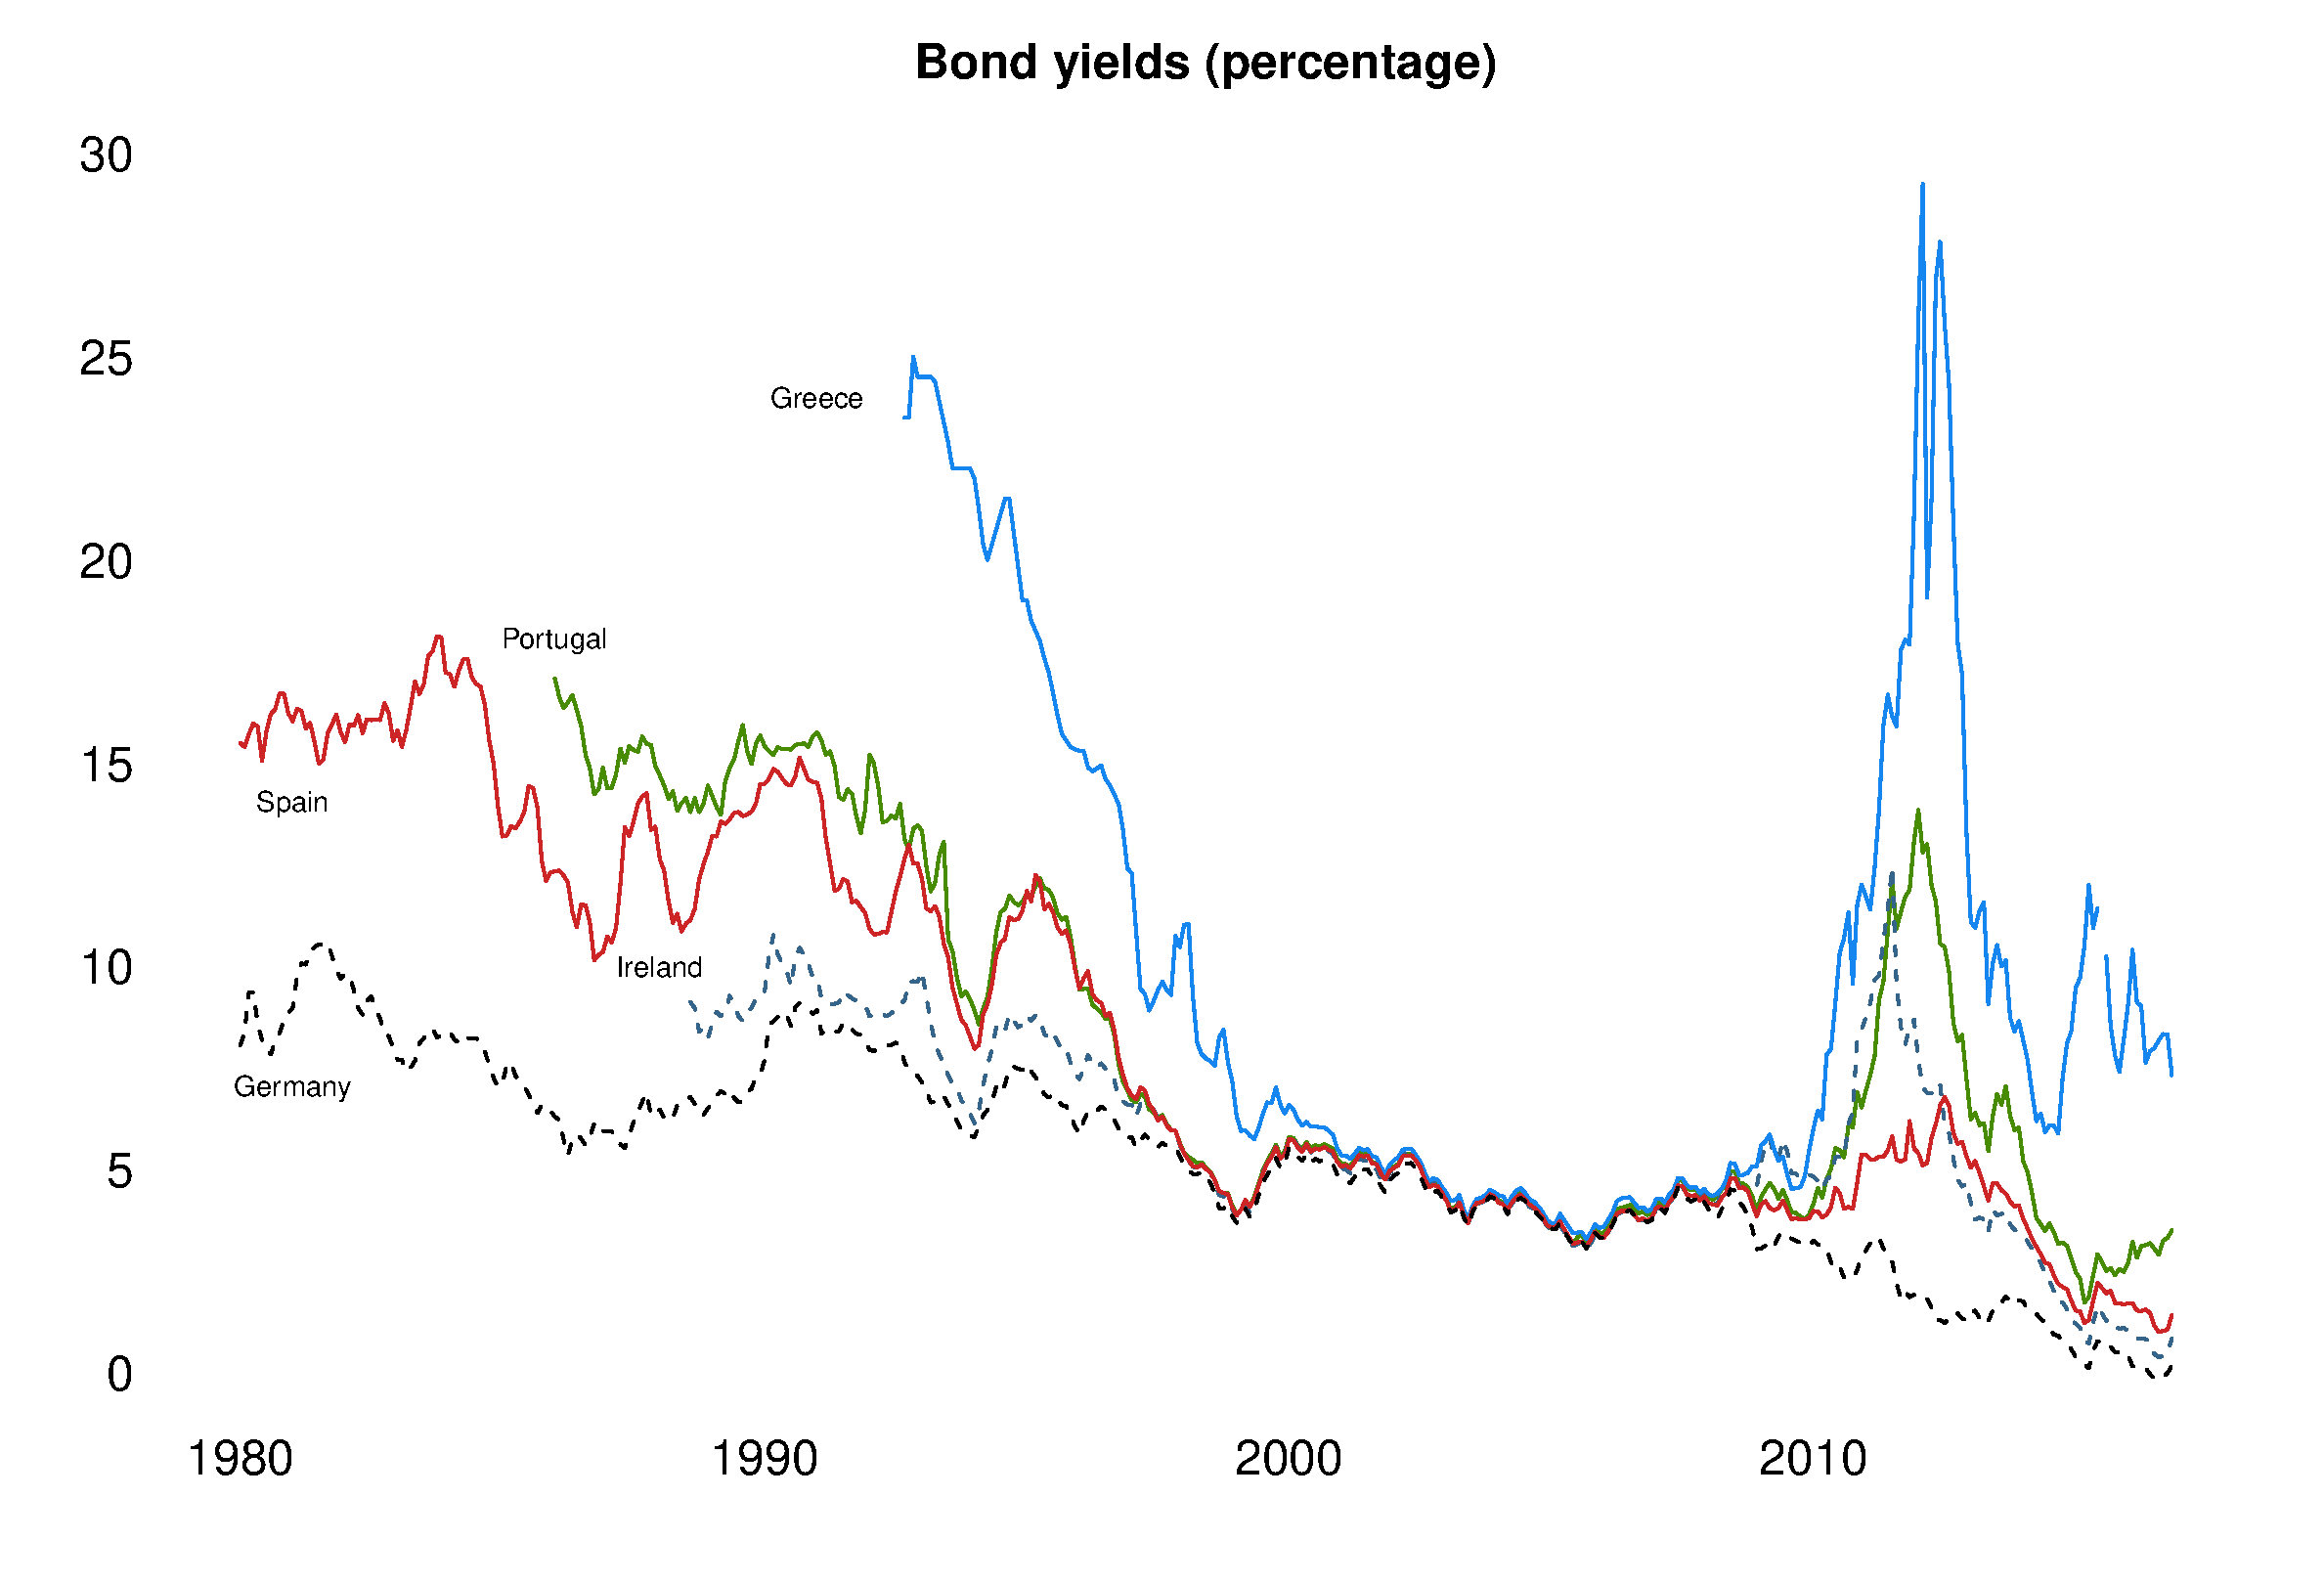
\includegraphics[scale=.3]{bond_yields.eps}
  \end{figure}
\end{frame}
%--------------------------------------

%--------------------------------------
\begin{frame}
  \begin{figure}
    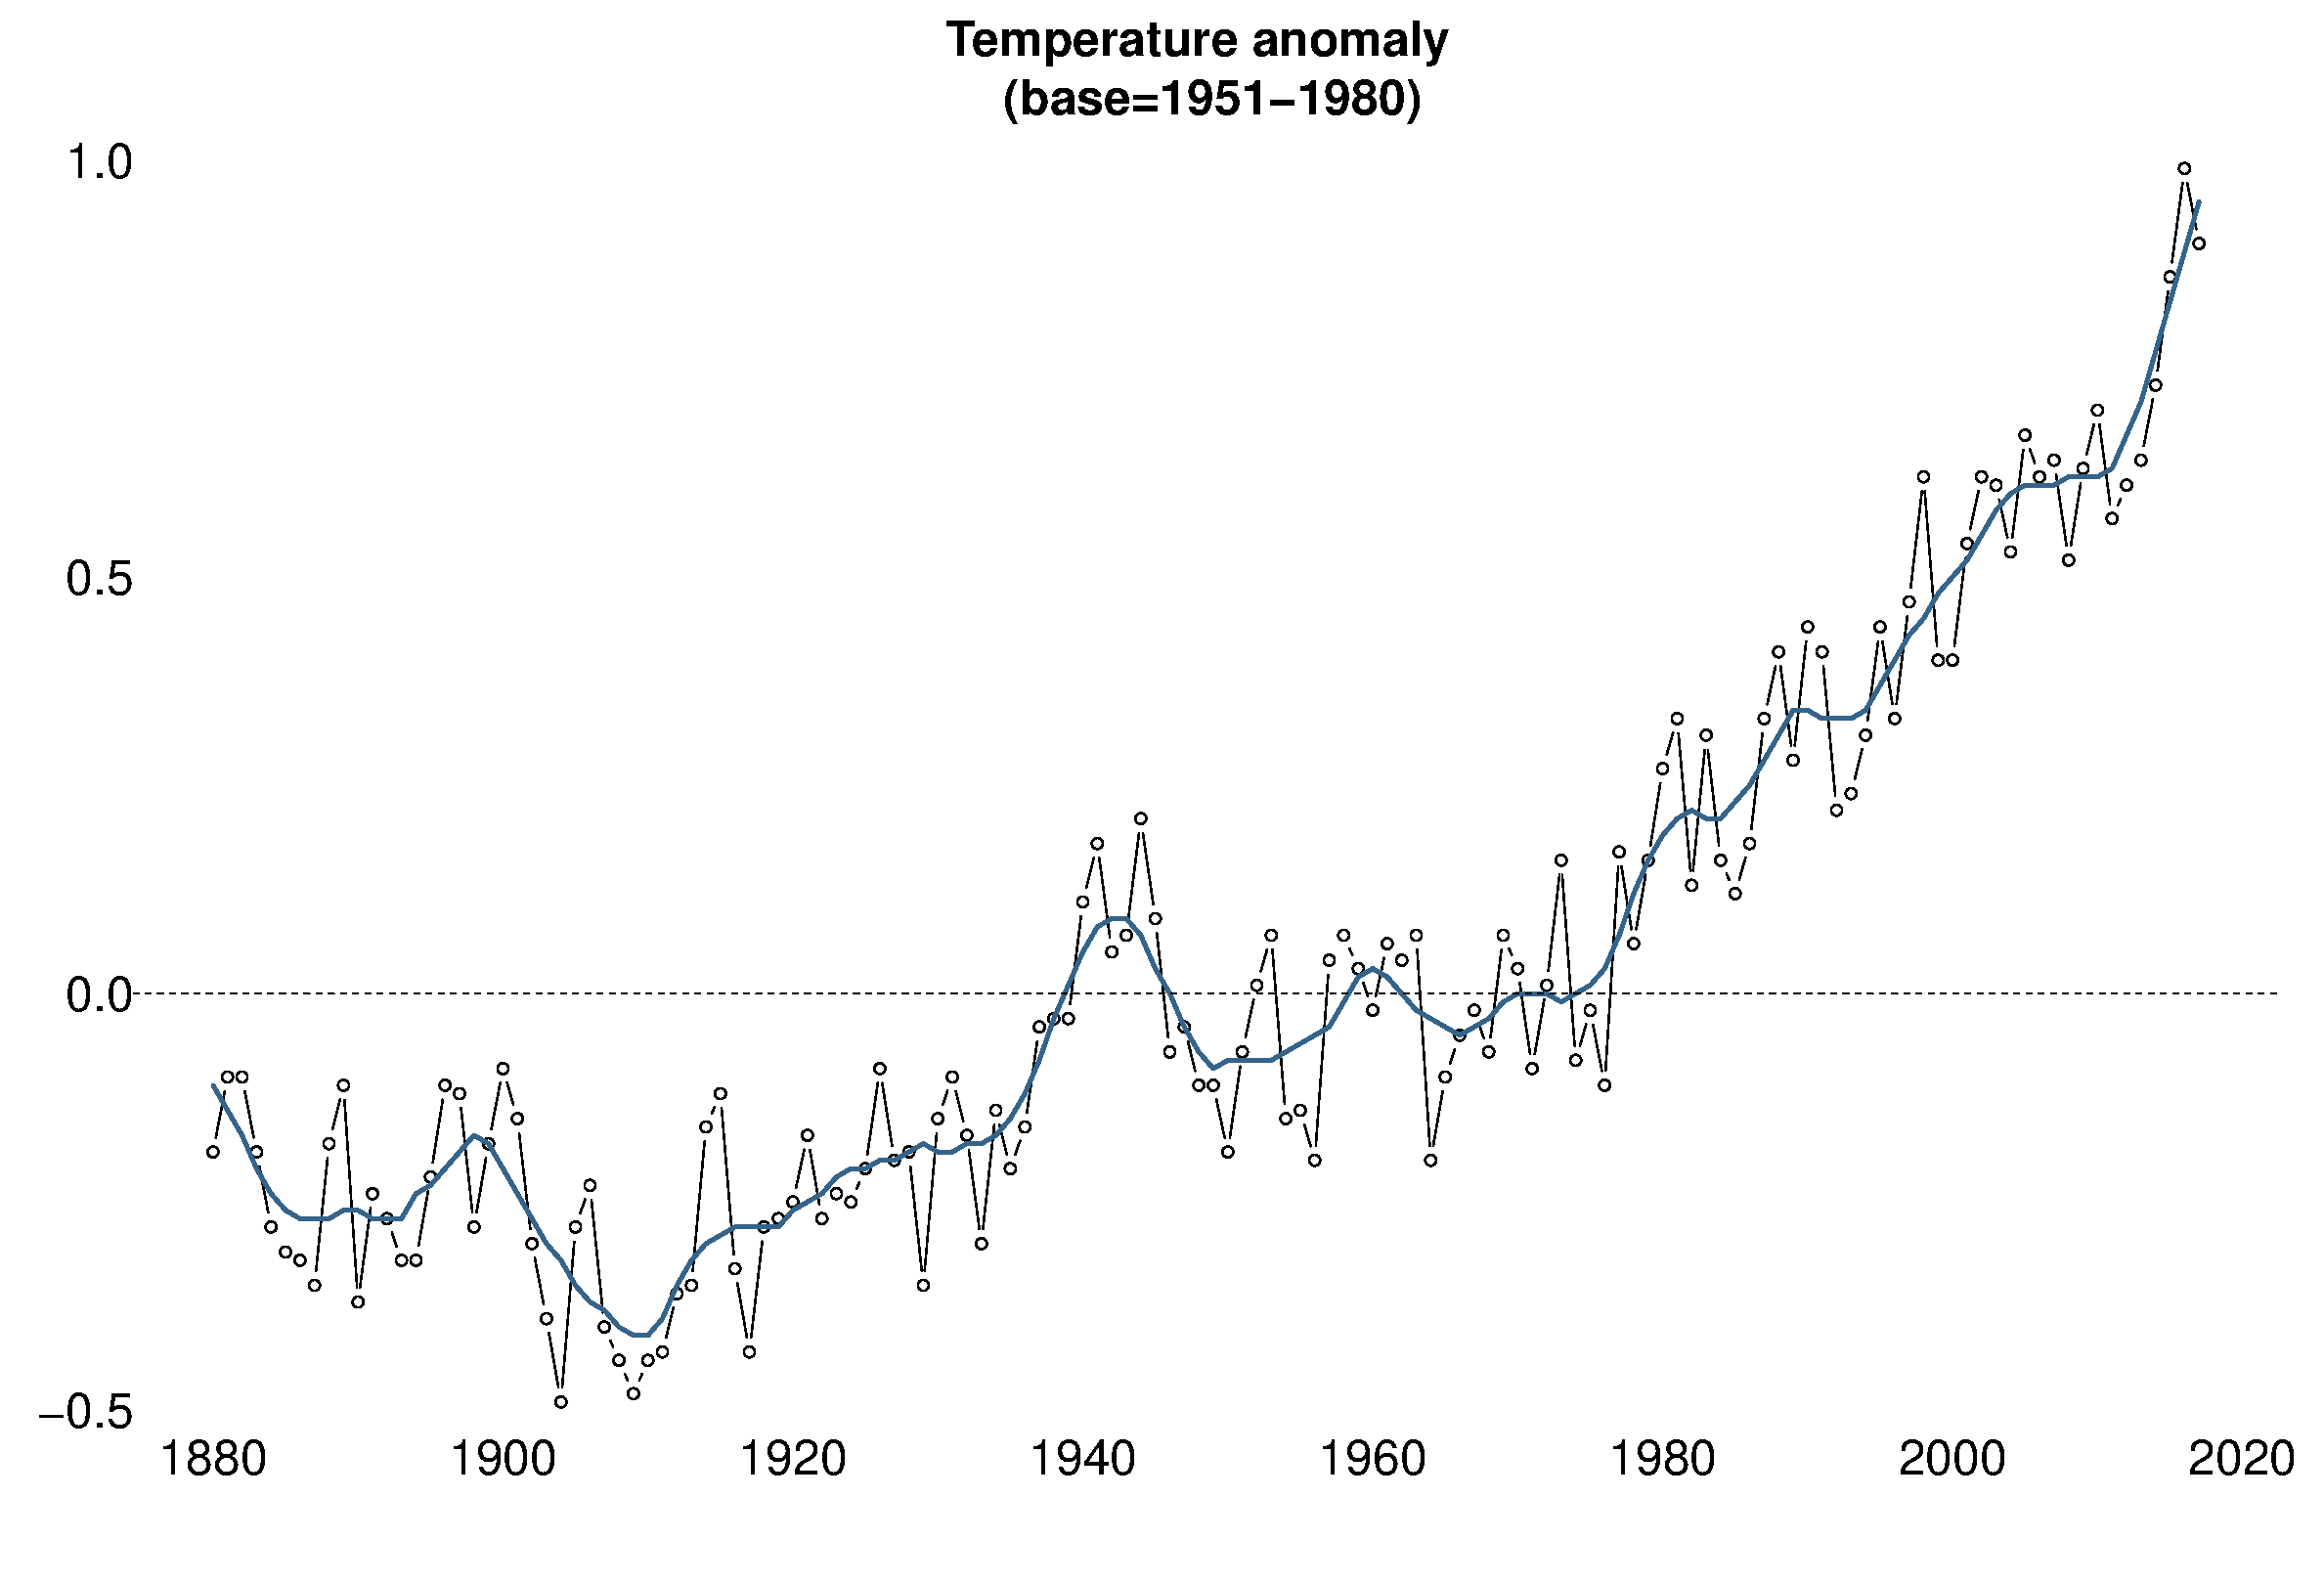
\includegraphics[scale=.25]{temperature.eps}
  \end{figure}
\end{frame}
%--------------------------------------

%--------------------------------------
\begin{frame}
  \begin{figure}
    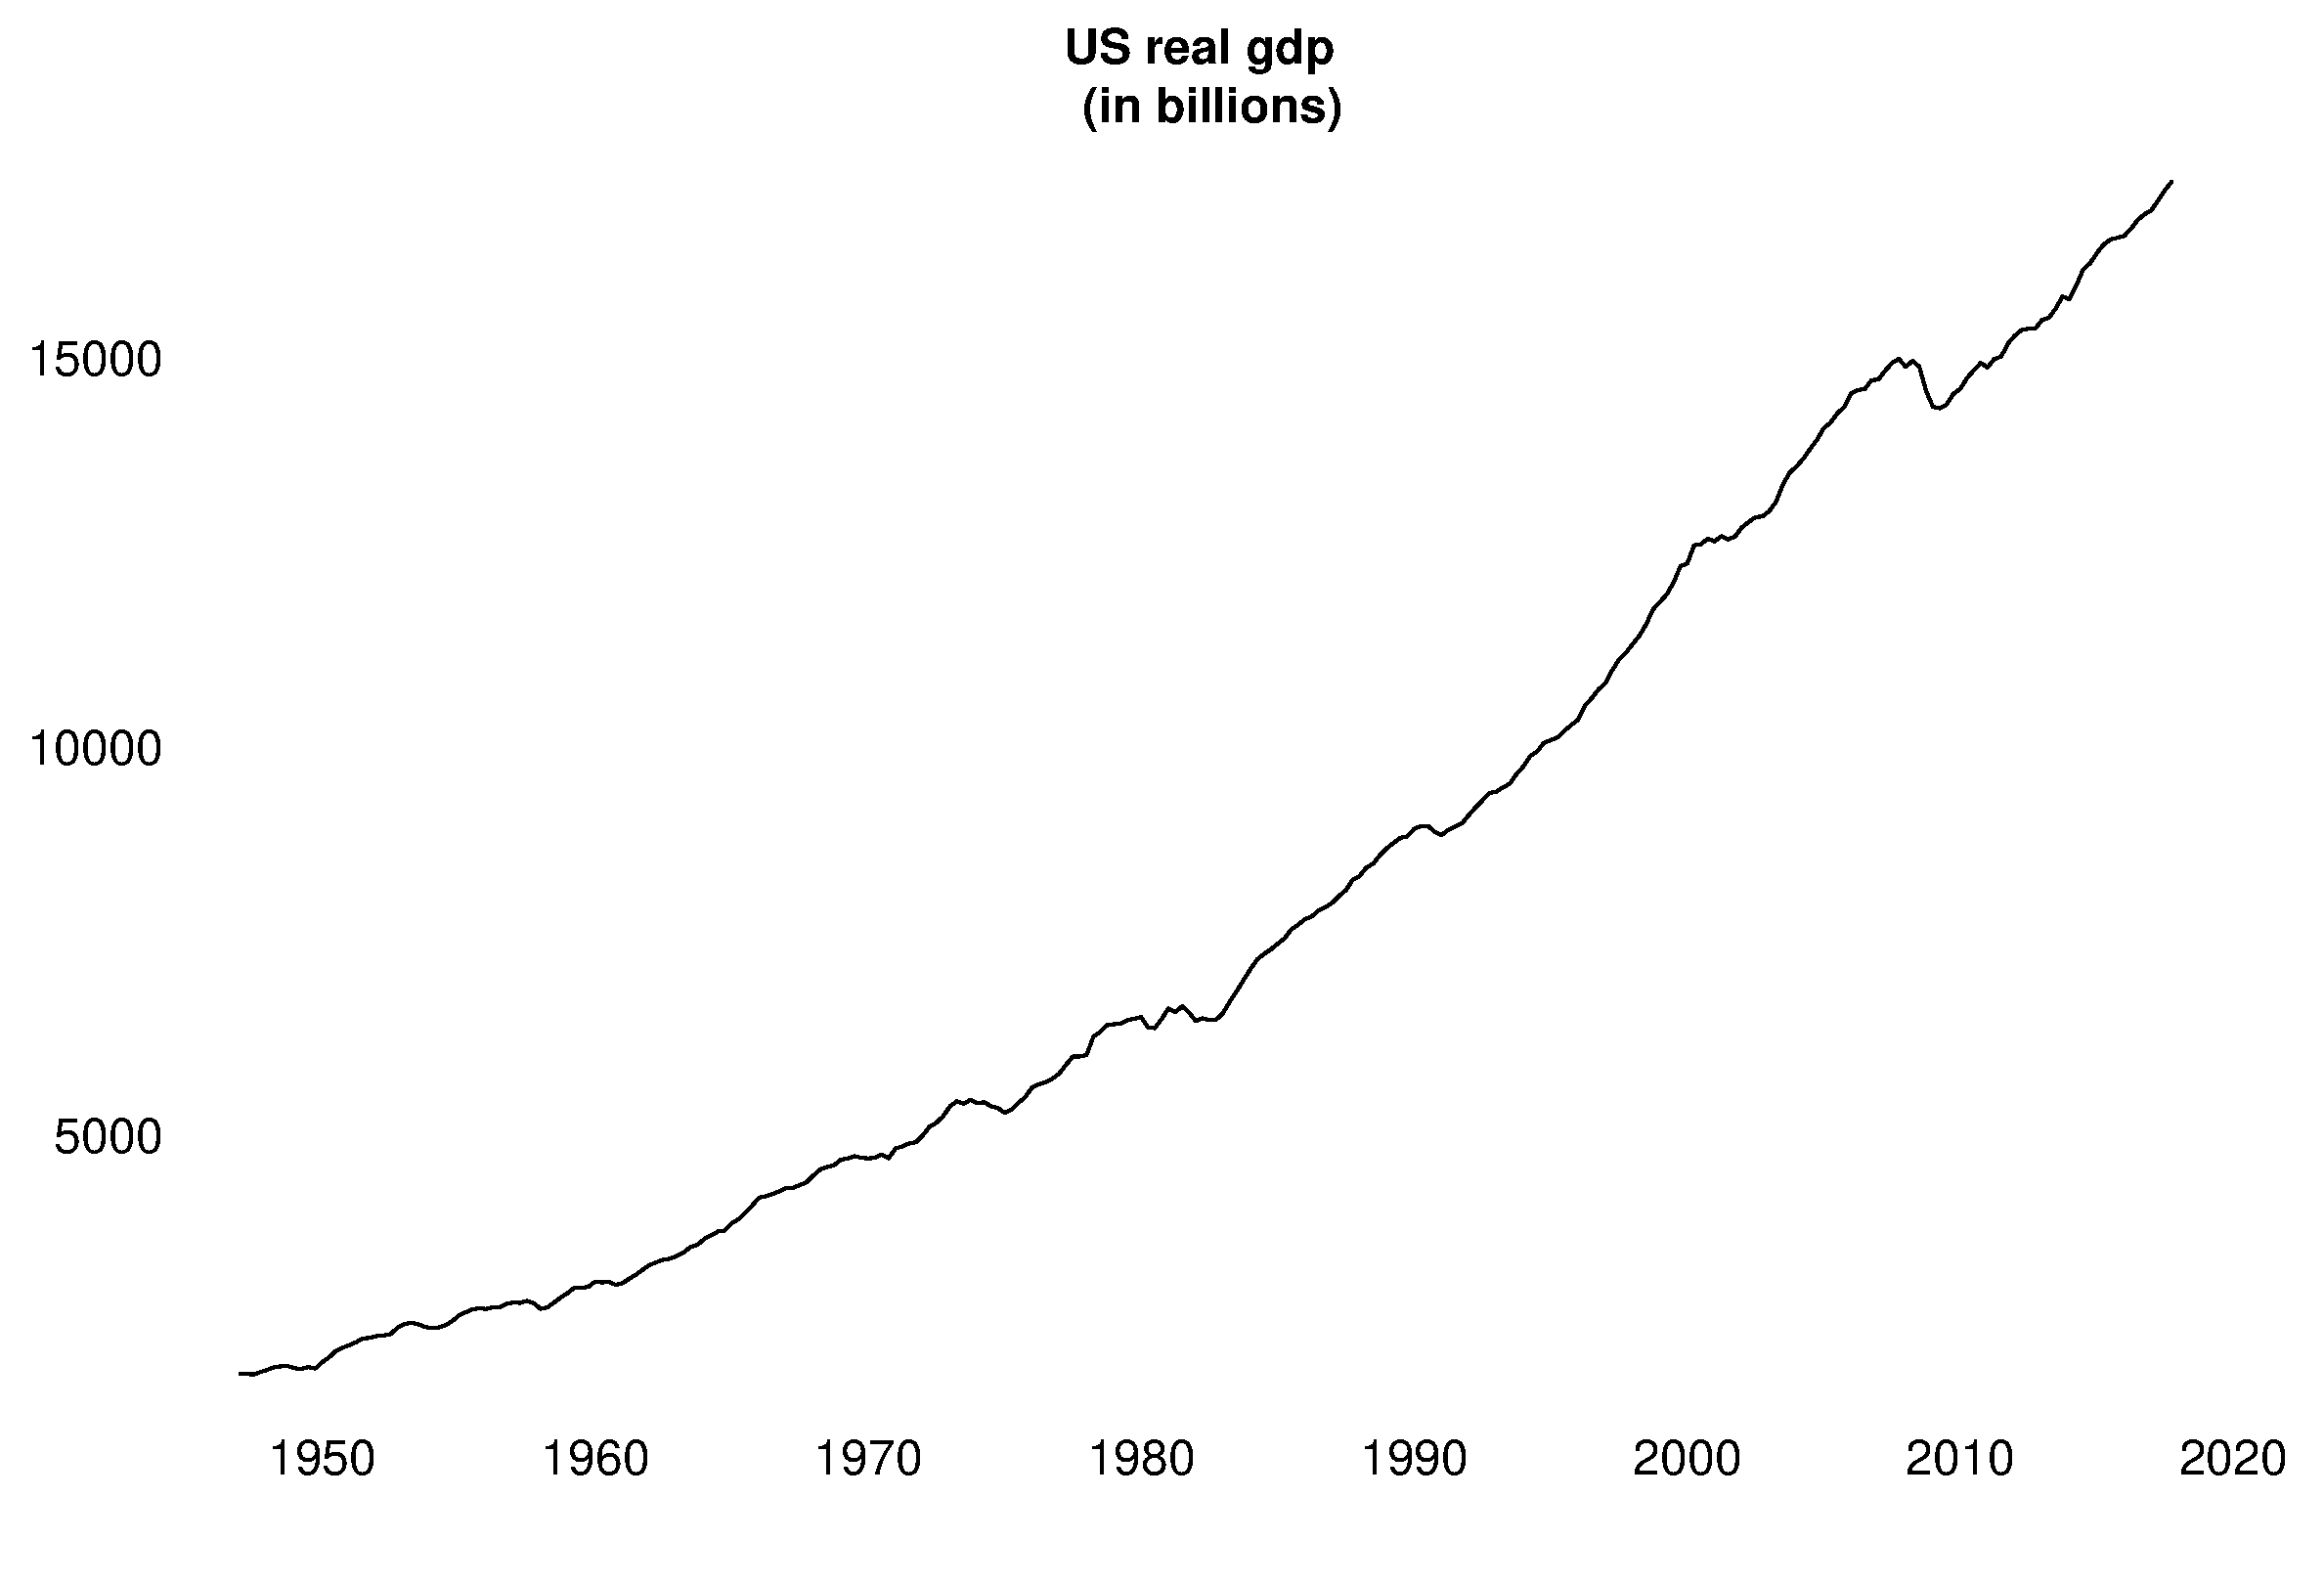
\includegraphics[scale=.25]{us_gdp.eps}
  \end{figure}
\end{frame}
%--------------------------------------

%--------------------------------------
\begin{frame}
  In general, time-series $Y_t$ for $t=1,2,...,T$ consists of  
 \begin{enumerate}
   \item Trend component $\tau_t$
   \item Cyclical component $c_t$
   \item Error component $\epsilon_t$
 \end{enumerate}
 \begin{align}
   y_t=\tau_t + c_t + \epsilon_t
 \end{align}
 \medskip
 What we are often interested in are the short-term fluctuations such as business cycles which means that the data has to be broken down into
  \begin{itemize}
    \item A non-stationary long-run trend, 
    \item A stationary cyclical component
  \end{itemize}  
\end{frame}
%--------------------------------------

%--------------------------------------
\begin{frame}
  \begin{figure}
    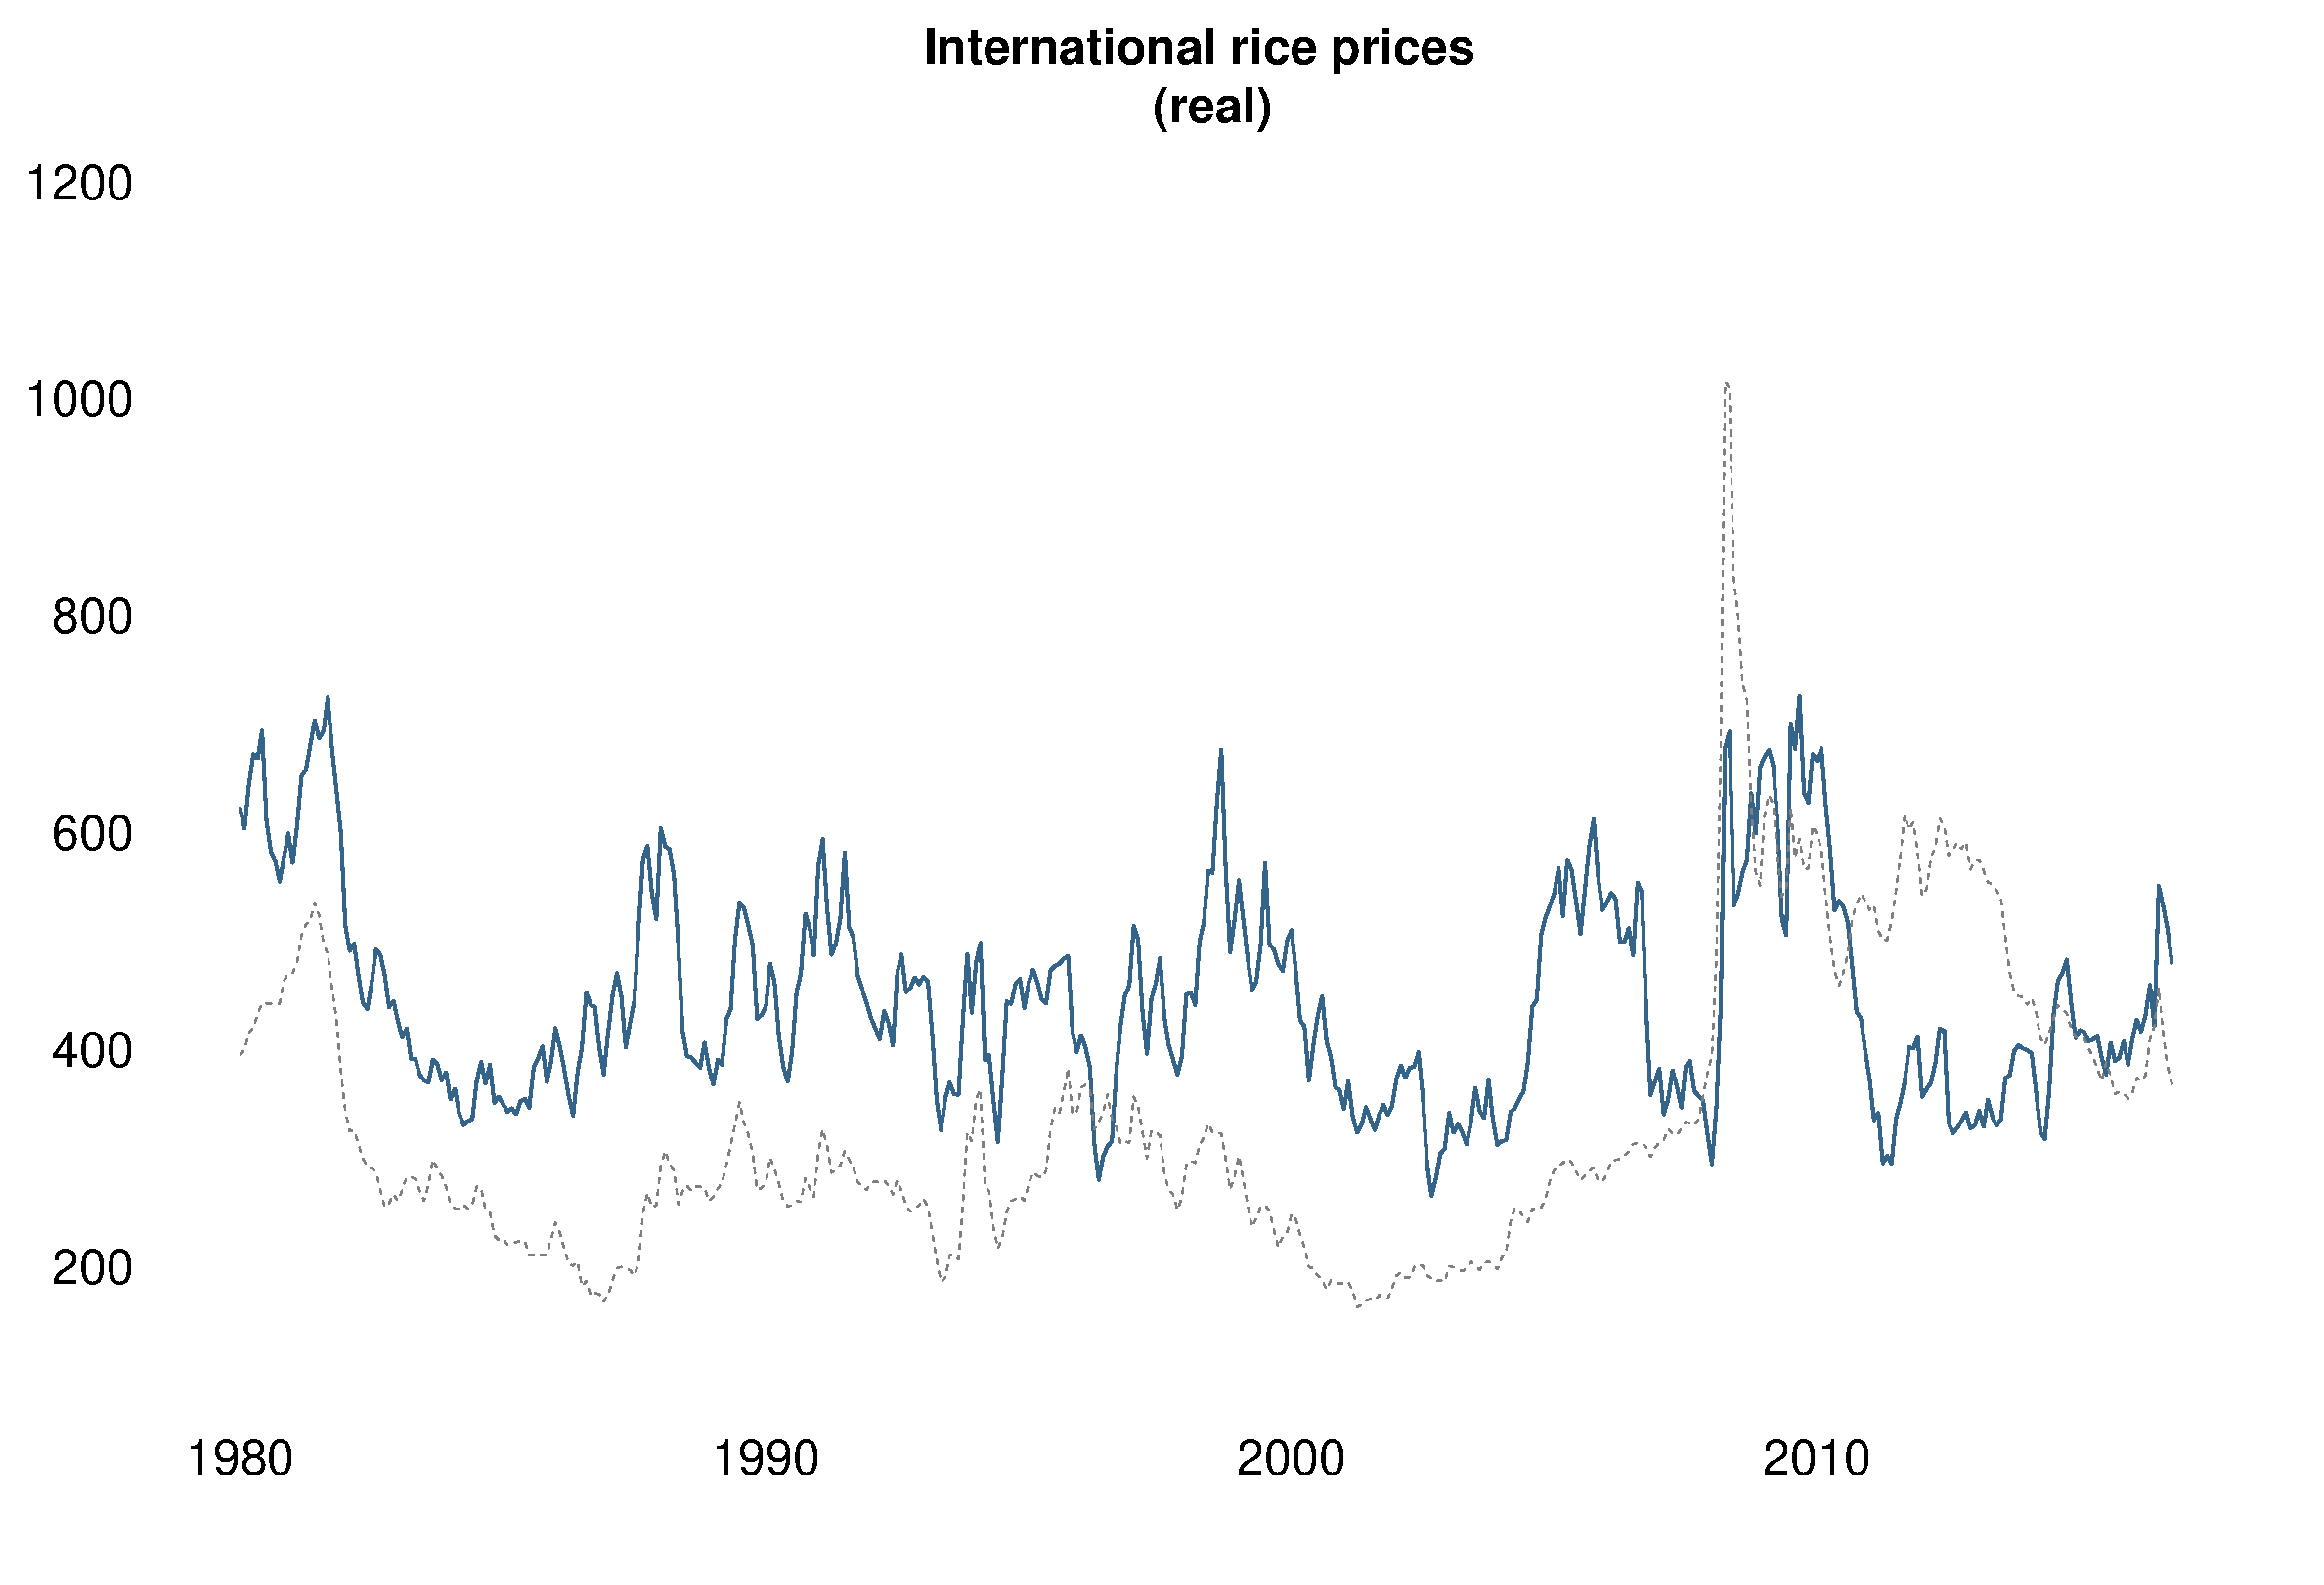
\includegraphics[scale=.3]{rice2.eps}
  \end{figure}
\end{frame}
%--------------------------------------

%--------------------------------------
\begin{frame}
  \begin{figure}
    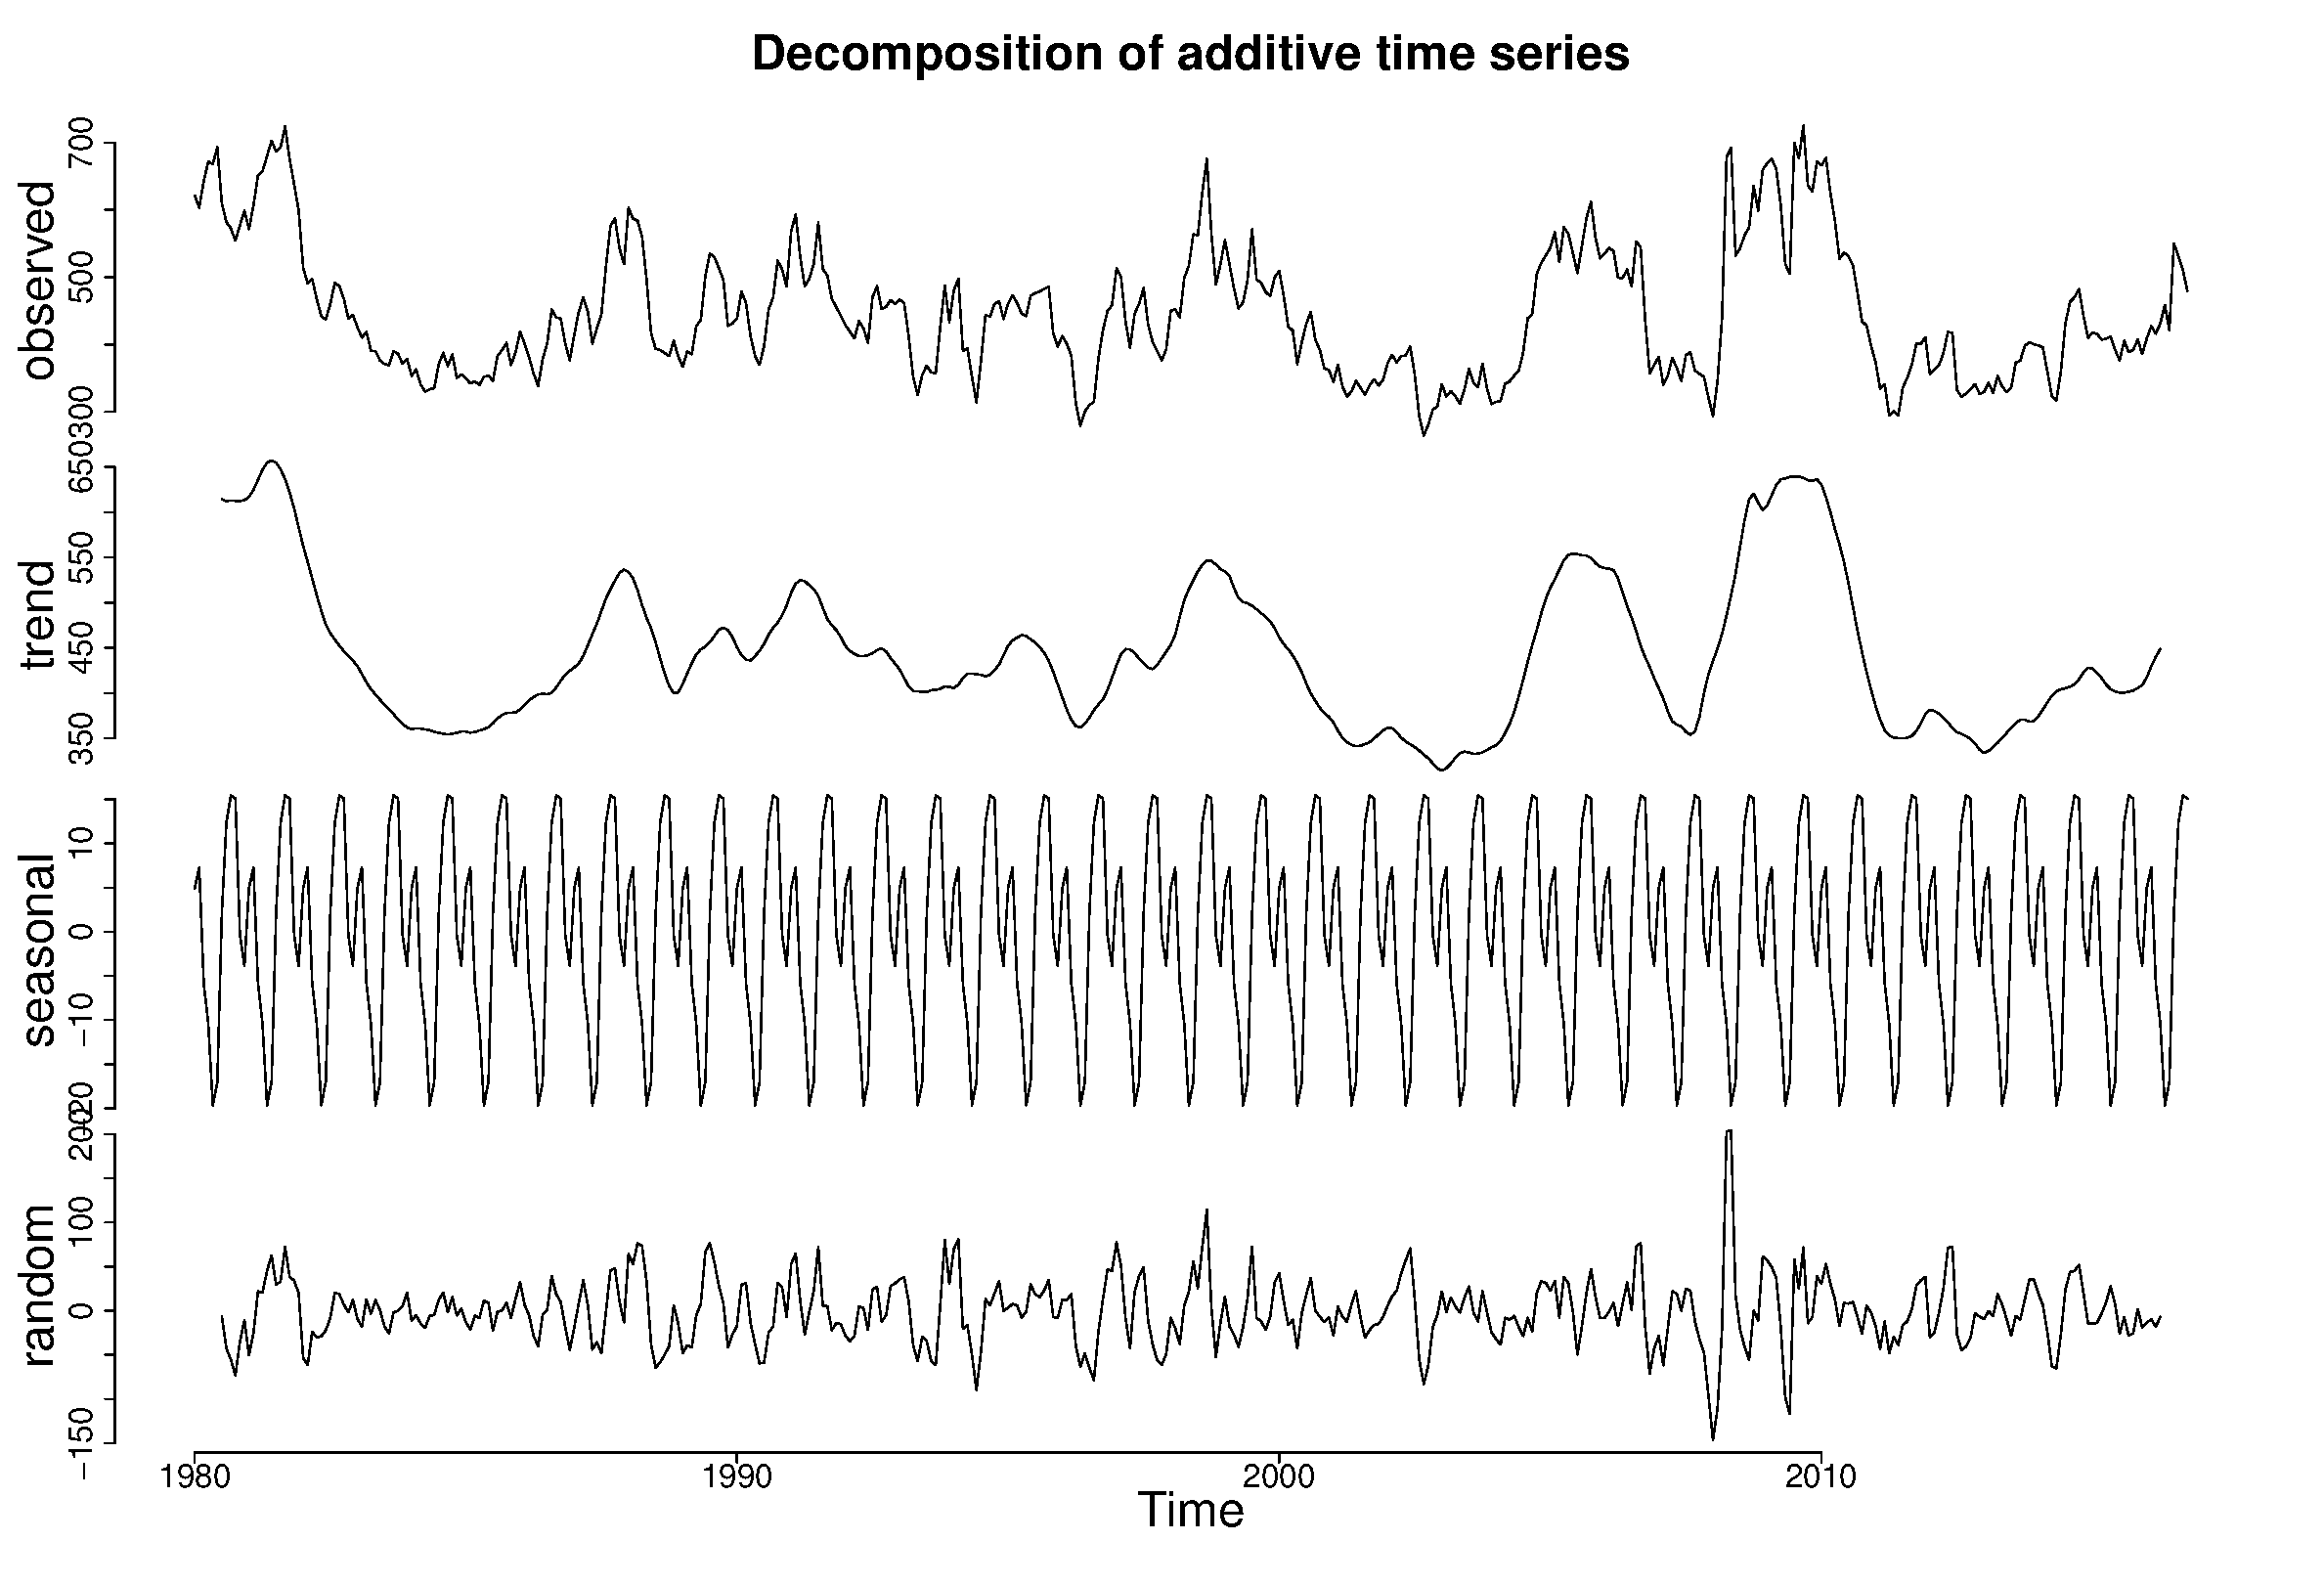
\includegraphics[scale=.3]{rice3.eps}
  \end{figure}
\end{frame}
%--------------------------------------

%--------------------------------------
\begin{frame}
  One of the simplest ways of detrending time-series data is using a log-linear model
  \begin{align}
    log Y_t = y_t = \alpha +gt + \epsilon_t
  \end{align}
  \medskip
  $\alpha+gt$ is the trend component\\
  $\epsilon$ is the stationary cyclical component (with zero mean)
\end{frame}
%--------------------------------------

%--------------------------------------
\begin{frame}
  \begin{figure}
    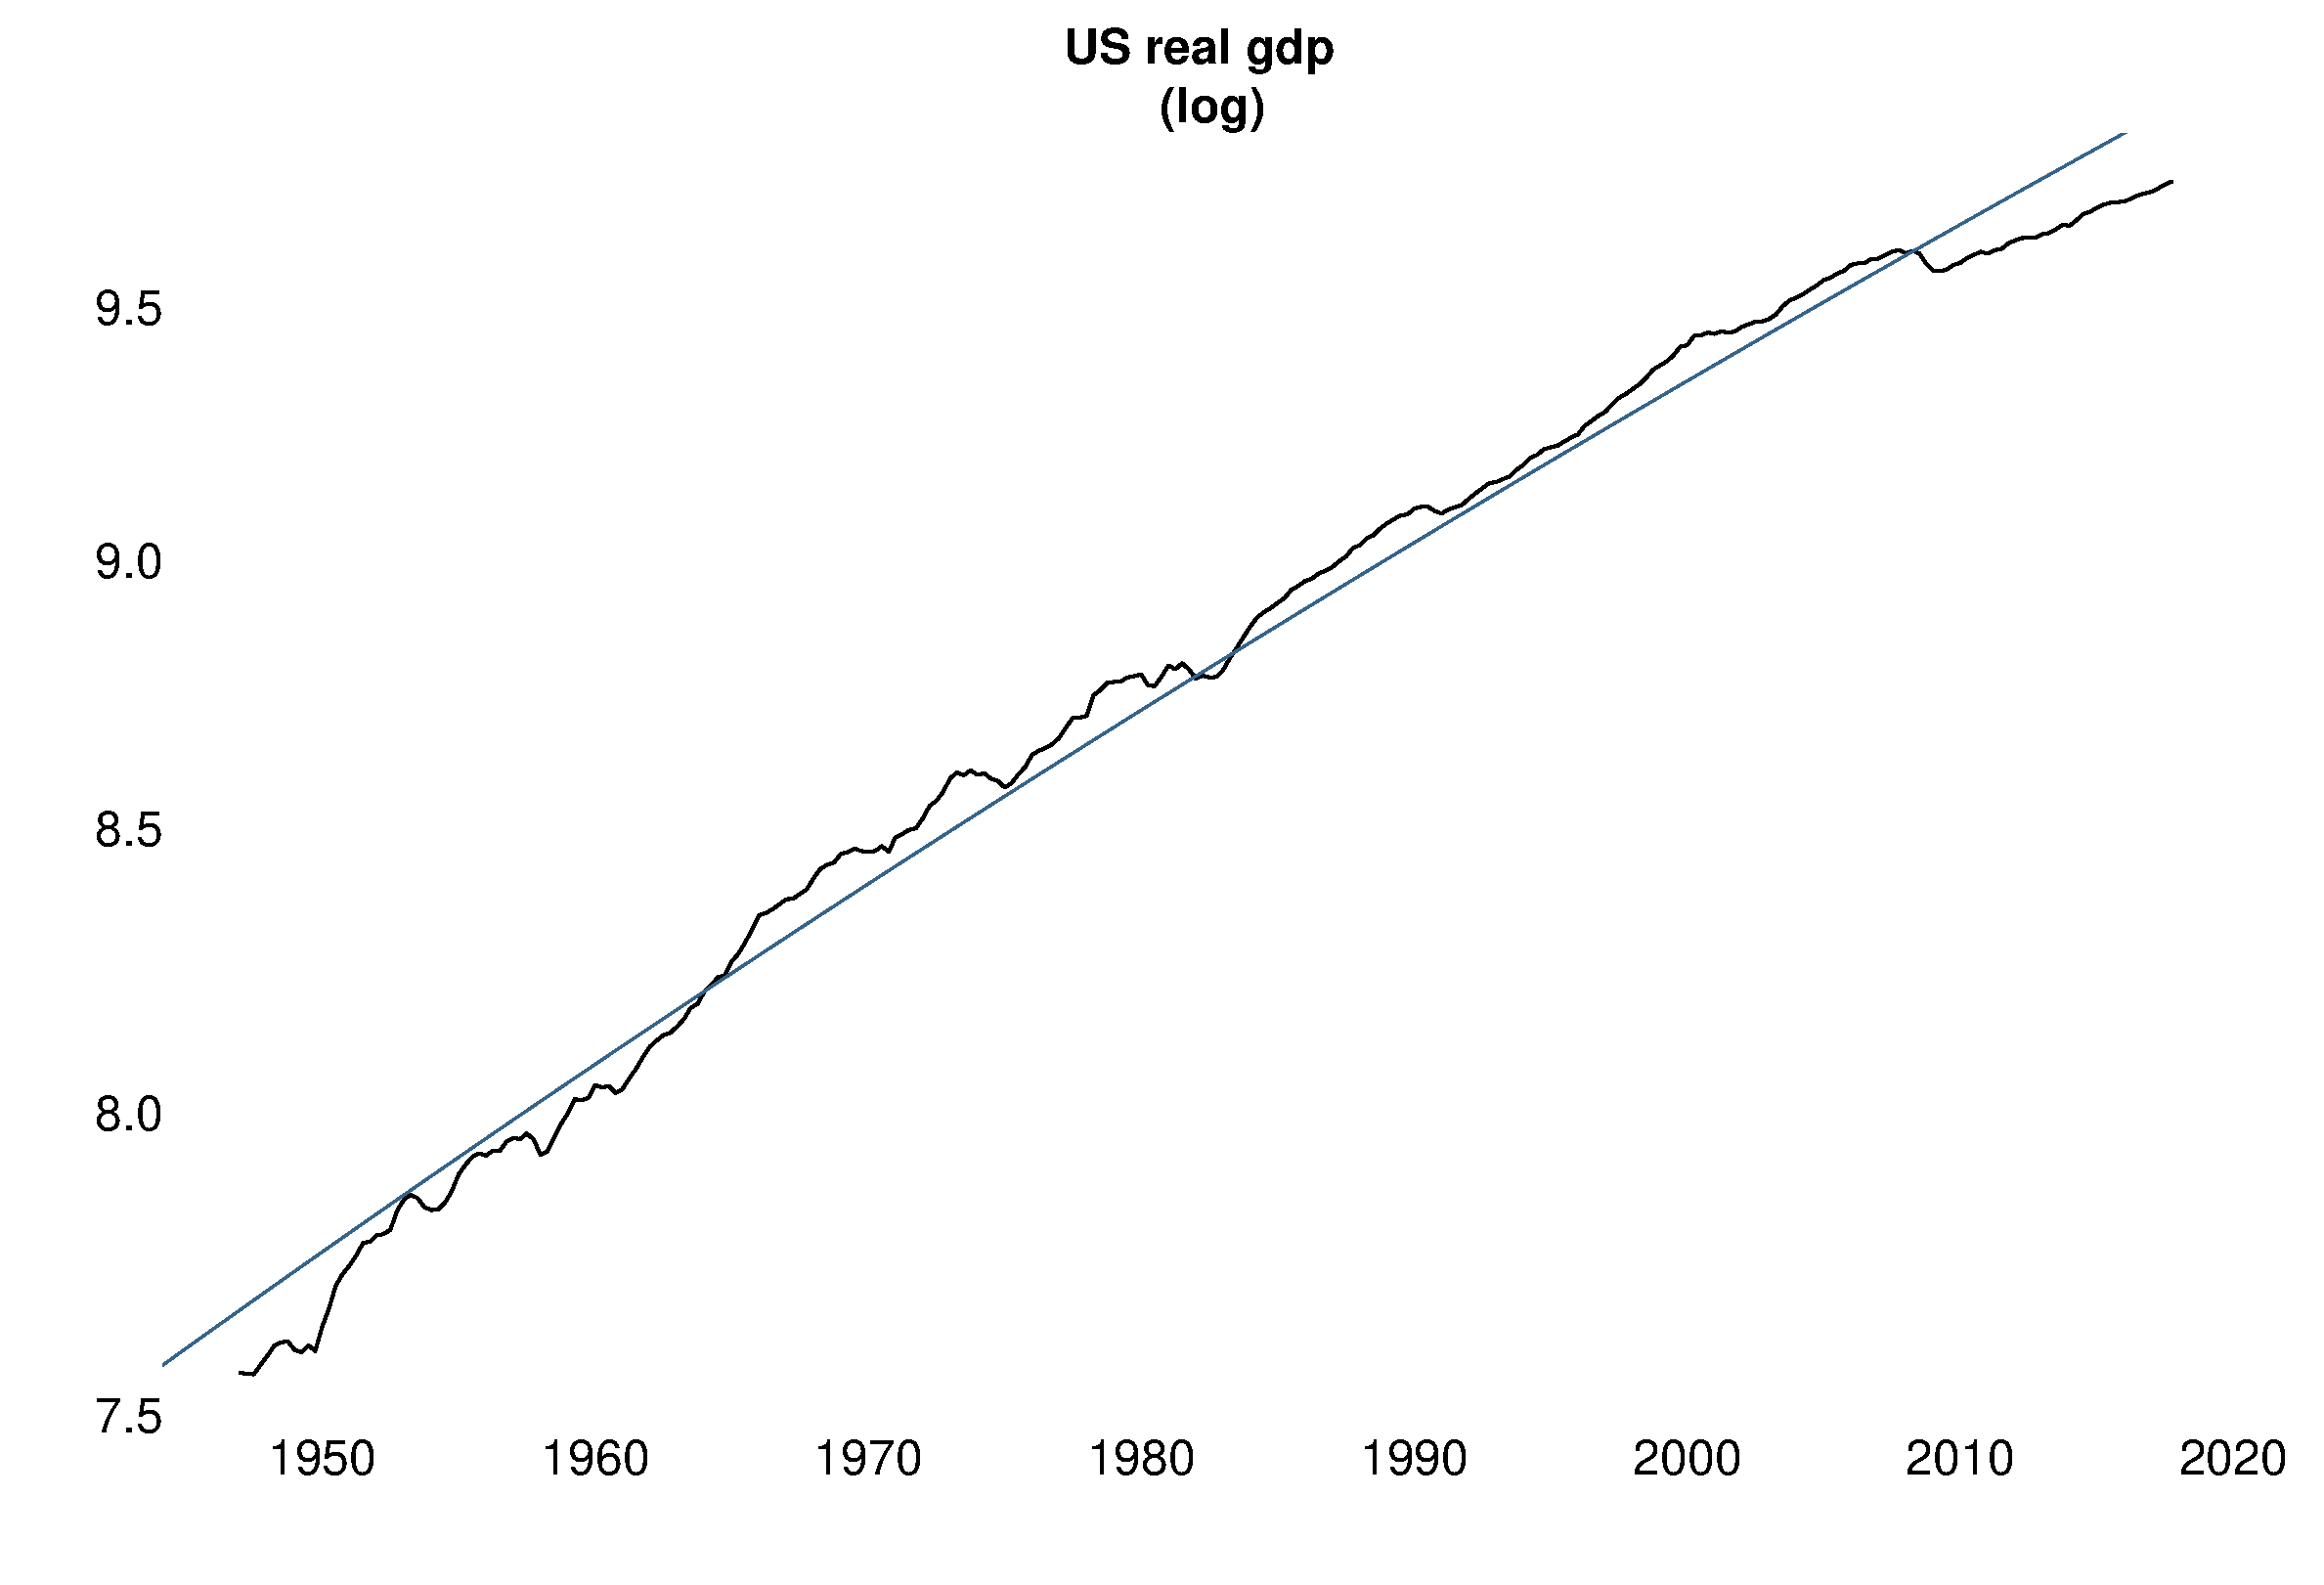
\includegraphics[scale=.3]{log_linear.eps}
  \end{figure}
\end{frame}
%--------------------------------------

%--------------------------------------
\begin{frame}
  \begin{figure}
    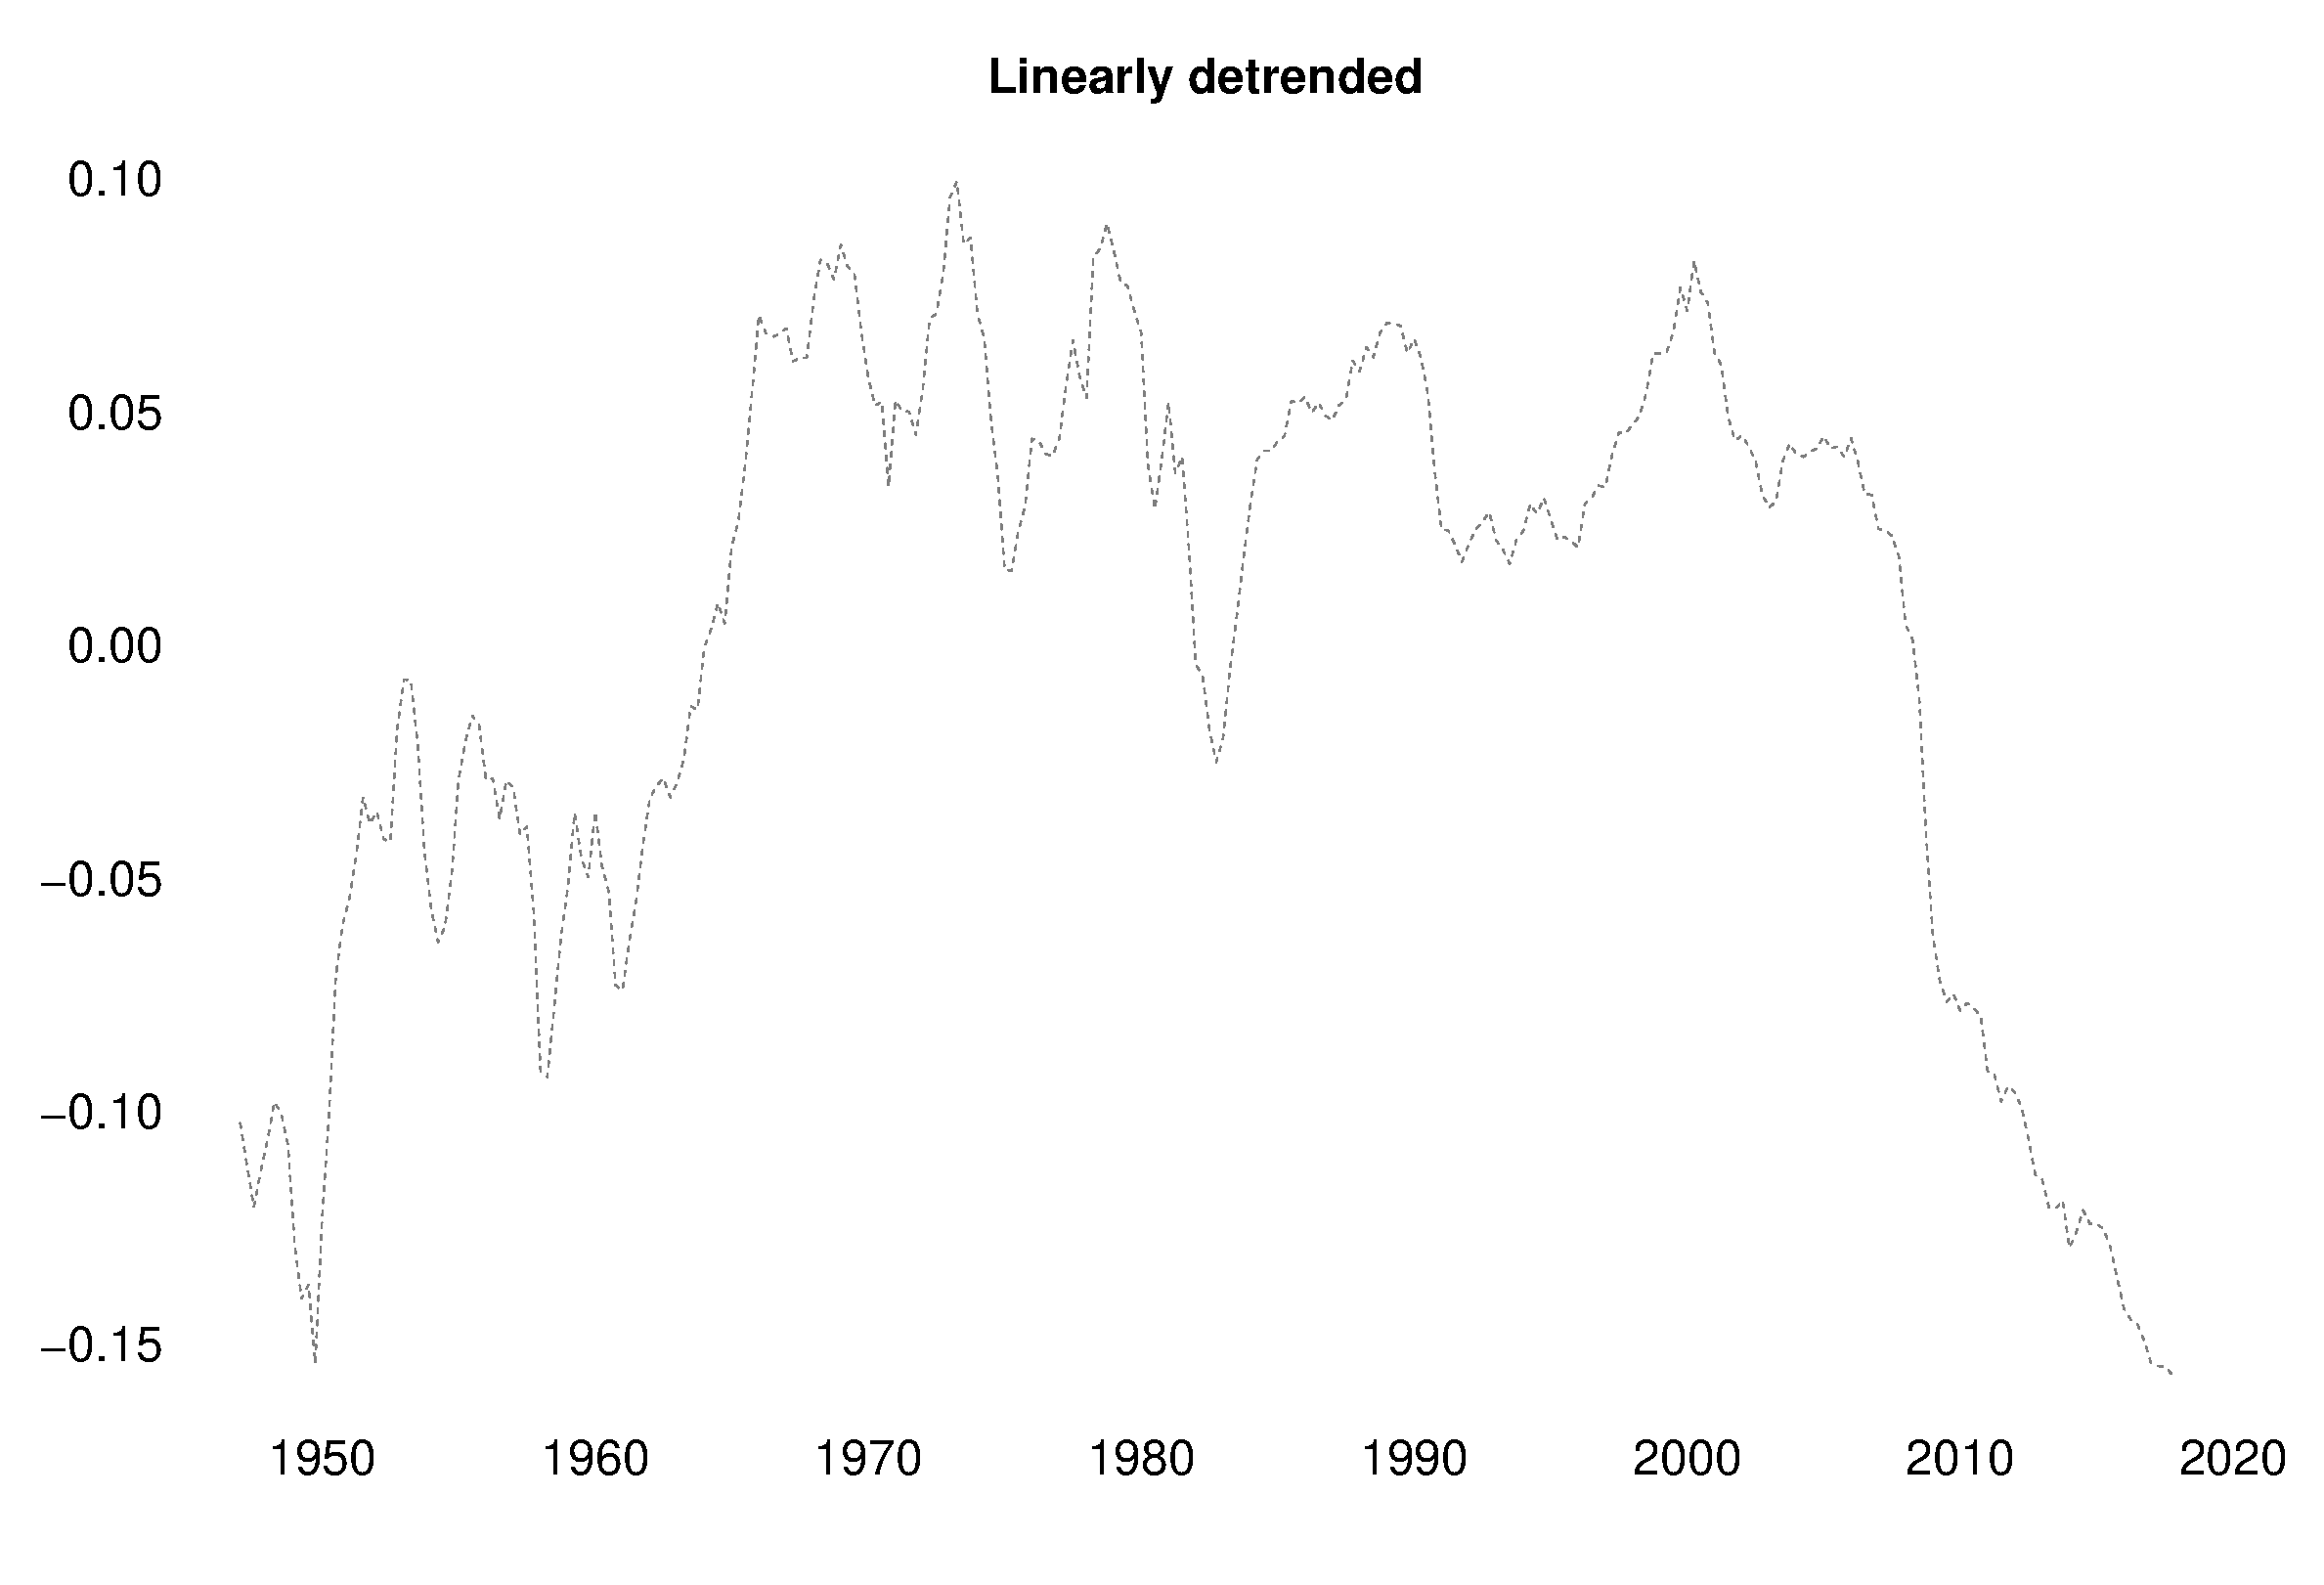
\includegraphics[scale=.3]{loglin_errors.eps}
  \end{figure}
\end{frame}
%--------------------------------------

%--------------------------------------
\begin{frame}
  Taking first-differences of log-transformed data will give something equivalent to the growth rate $\Delta y_t$ which comprises of
  \begin{enumerate}
    \item Constant trend growth $g$
    \item Change in cyclical component $\Delta \epsilon_t$
  \end{enumerate}
\end{frame}
%--------------------------------------

%--------------------------------------
\begin{frame}
  \begin{figure}
    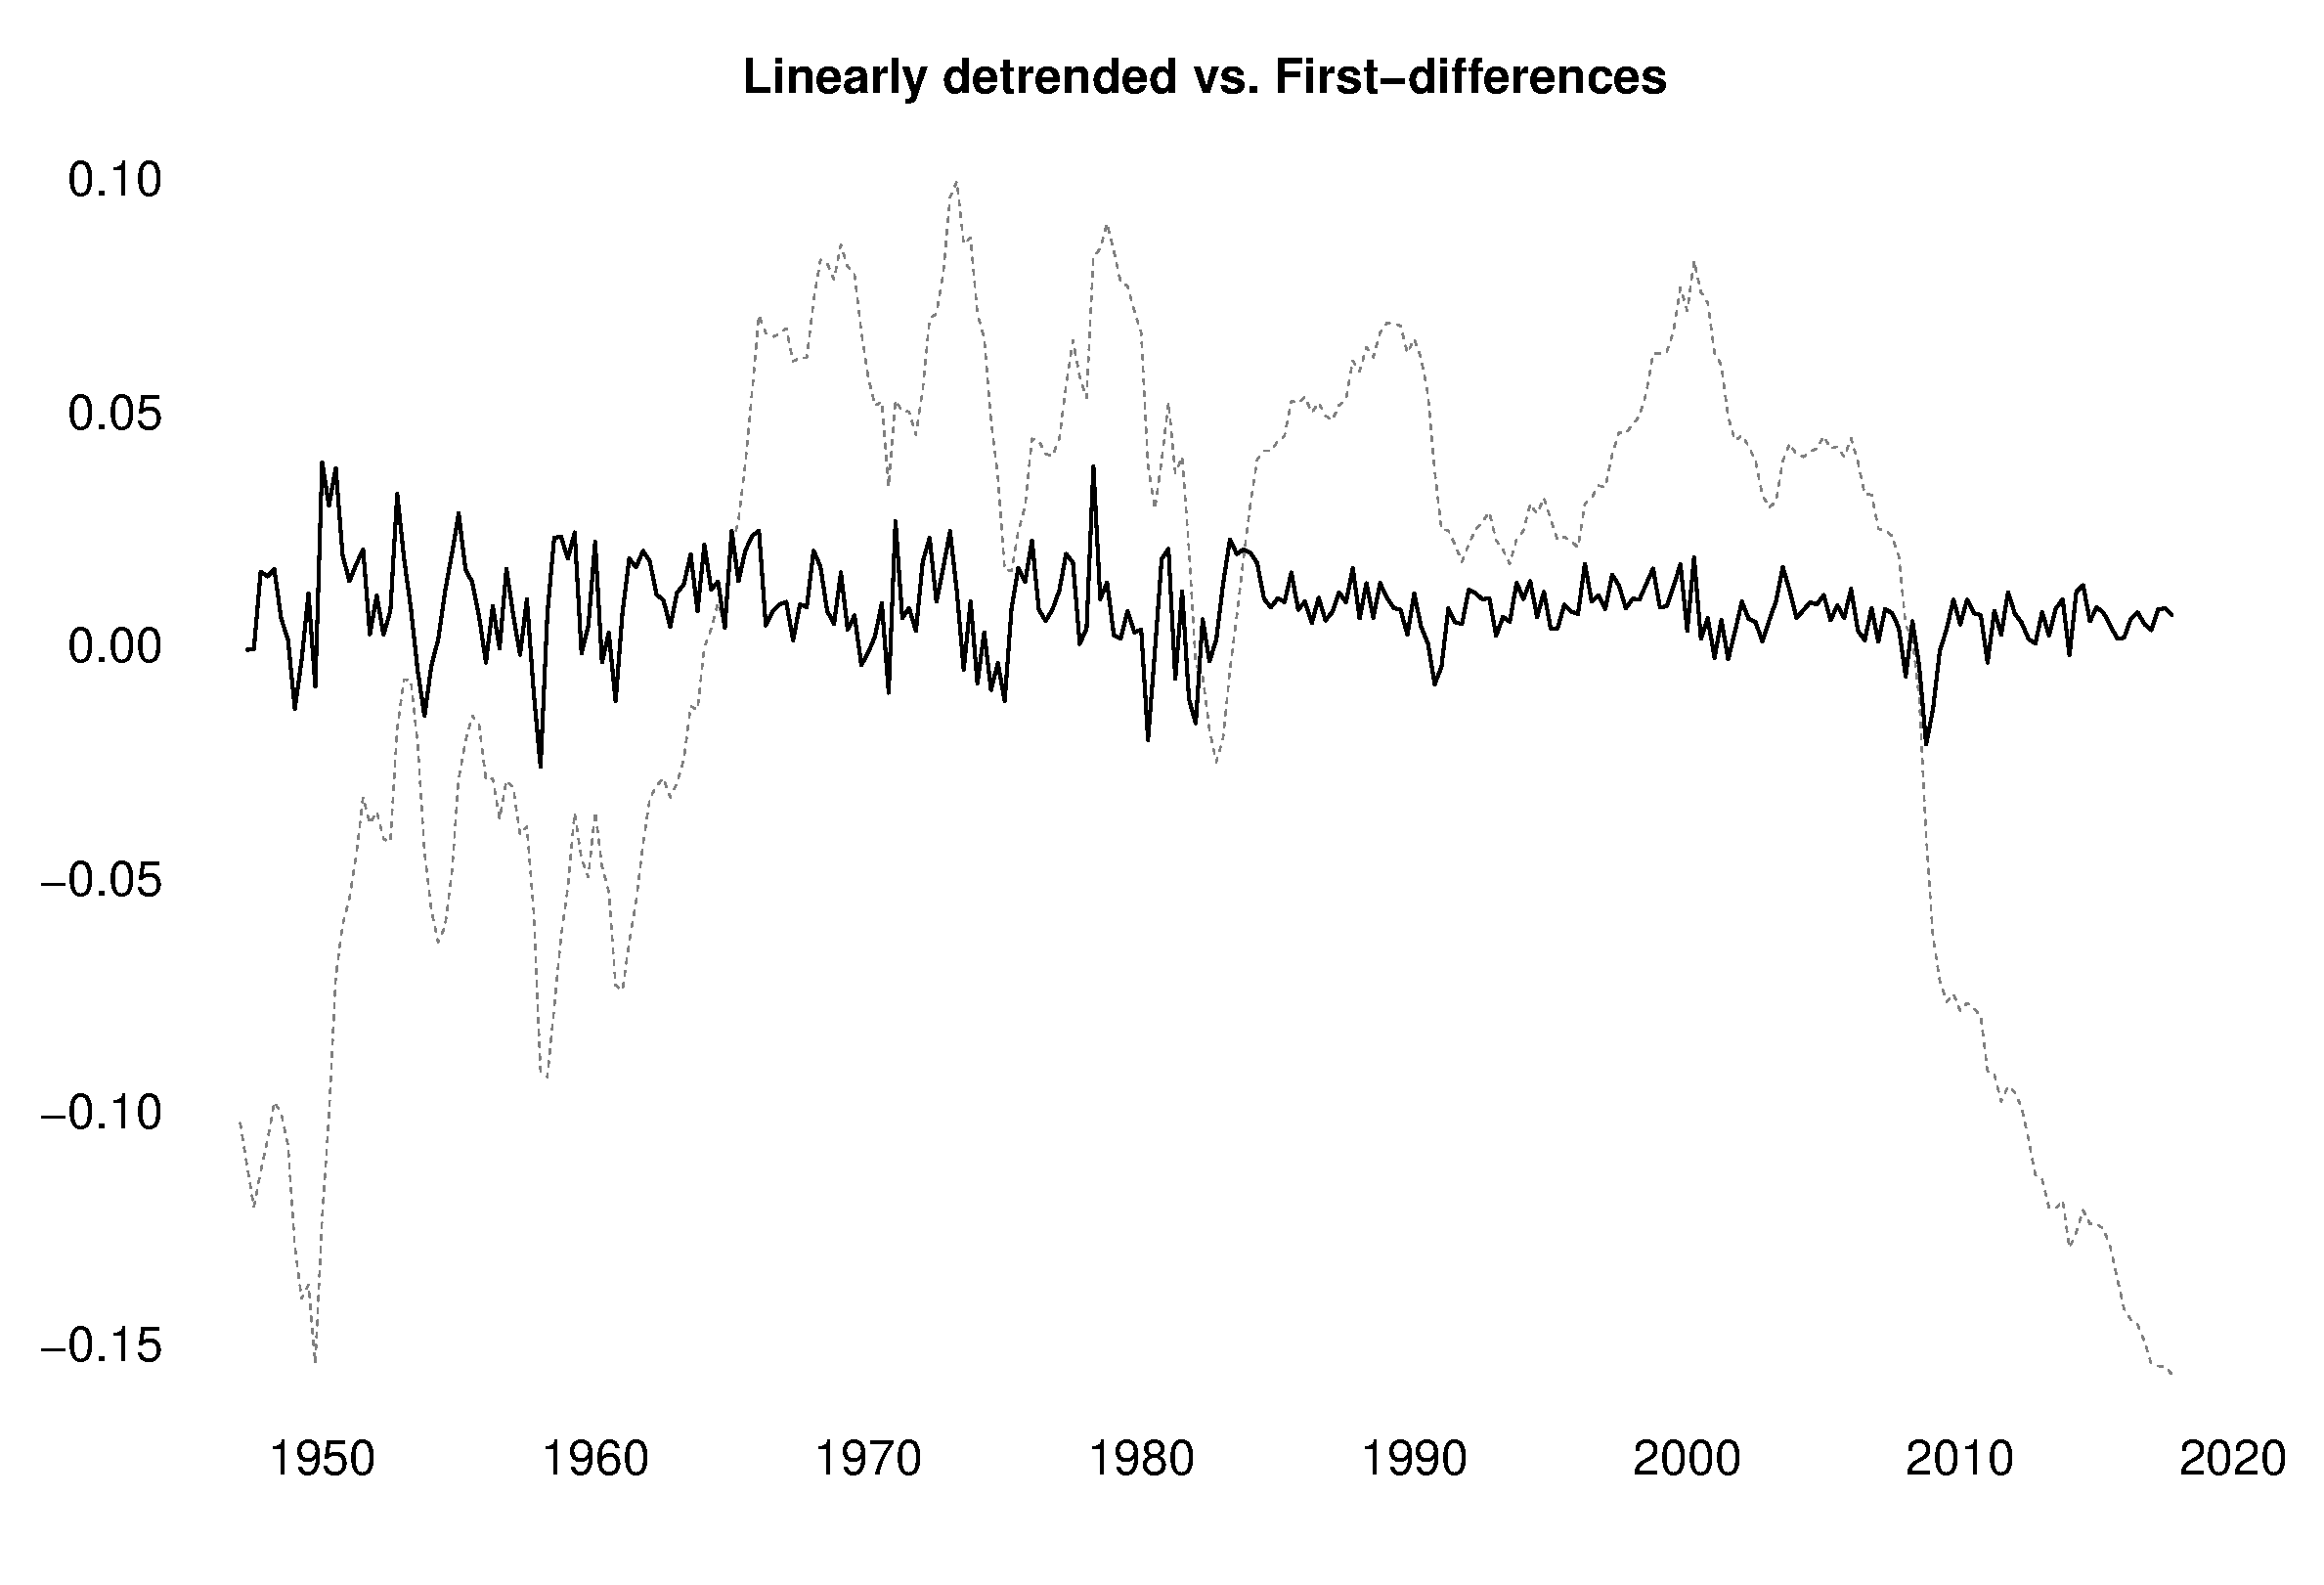
\includegraphics[scale=.3]{first_differences.eps}
  \end{figure}
\end{frame}
%--------------------------------------

%--------------------------------------
\begin{frame}
 For ease of notation let $y_t$ be our time-series, can write growth as  
  \begin{align}
    \Delta y_t = \frac{y_t - y_{t-1}}{y_{t-1}}    
  \end{align}
  \medskip
  Taking logs of growth rate gives   
  \begin{align}
    \Delta y_t= log\; y_t - log\; y_{t-1}
  \end{align}    
\end{frame}
%--------------------------------------

%--------------------------------------
\begin{frame}  
  \begin{align}
    log\; y_t-log\; y_{t-1} &= log\left(\frac{y_t}{y_{t-1}}\right) \\ \nonumber
    & \approx \frac{y_t}{y_{t-1}}-1\\ \nonumber
    &= \frac{y_t}{y_{t-1}}-\frac{y_{t-1}}{y_{t-1}}\\ \nonumber
    &= \frac{y_t - y_{t-1}}{y_{t-1}}      
  \end{align}
  \medskip
  \textbf{NB-} If $y$ is close to 1, this means that $log\;y$ will be close to $y-1$, and $\frac{y_t}{y_{t-1}}$ is likely close to 0  
\end{frame}
%--------------------------------------

%--------------------------------------
\begin{frame}
 Although straightforward, there is a caveat using a straight line to detrend the data.
 Suppose that the correct model is
\begin{align}
 y_t = g+ y_{t-1} + \epsilon_t
\end{align}
\medskip
Recall that growth has a constant component $g$ and random component $\epsilon_t$: two important implications
\begin{enumerate}
  \item Cycles are the accumulation of all the random shock over time that affected $\Delta y_t$
  \item Expected growth rate will be $g$; irrespective of what happened in the past
\end{enumerate}
\medskip
\textbf{NB-}Another issue is medium-run changes in $g$
\end{frame}
%--------------------------------------

%--------------------------------------
\begin{frame}
  \begin{figure}
    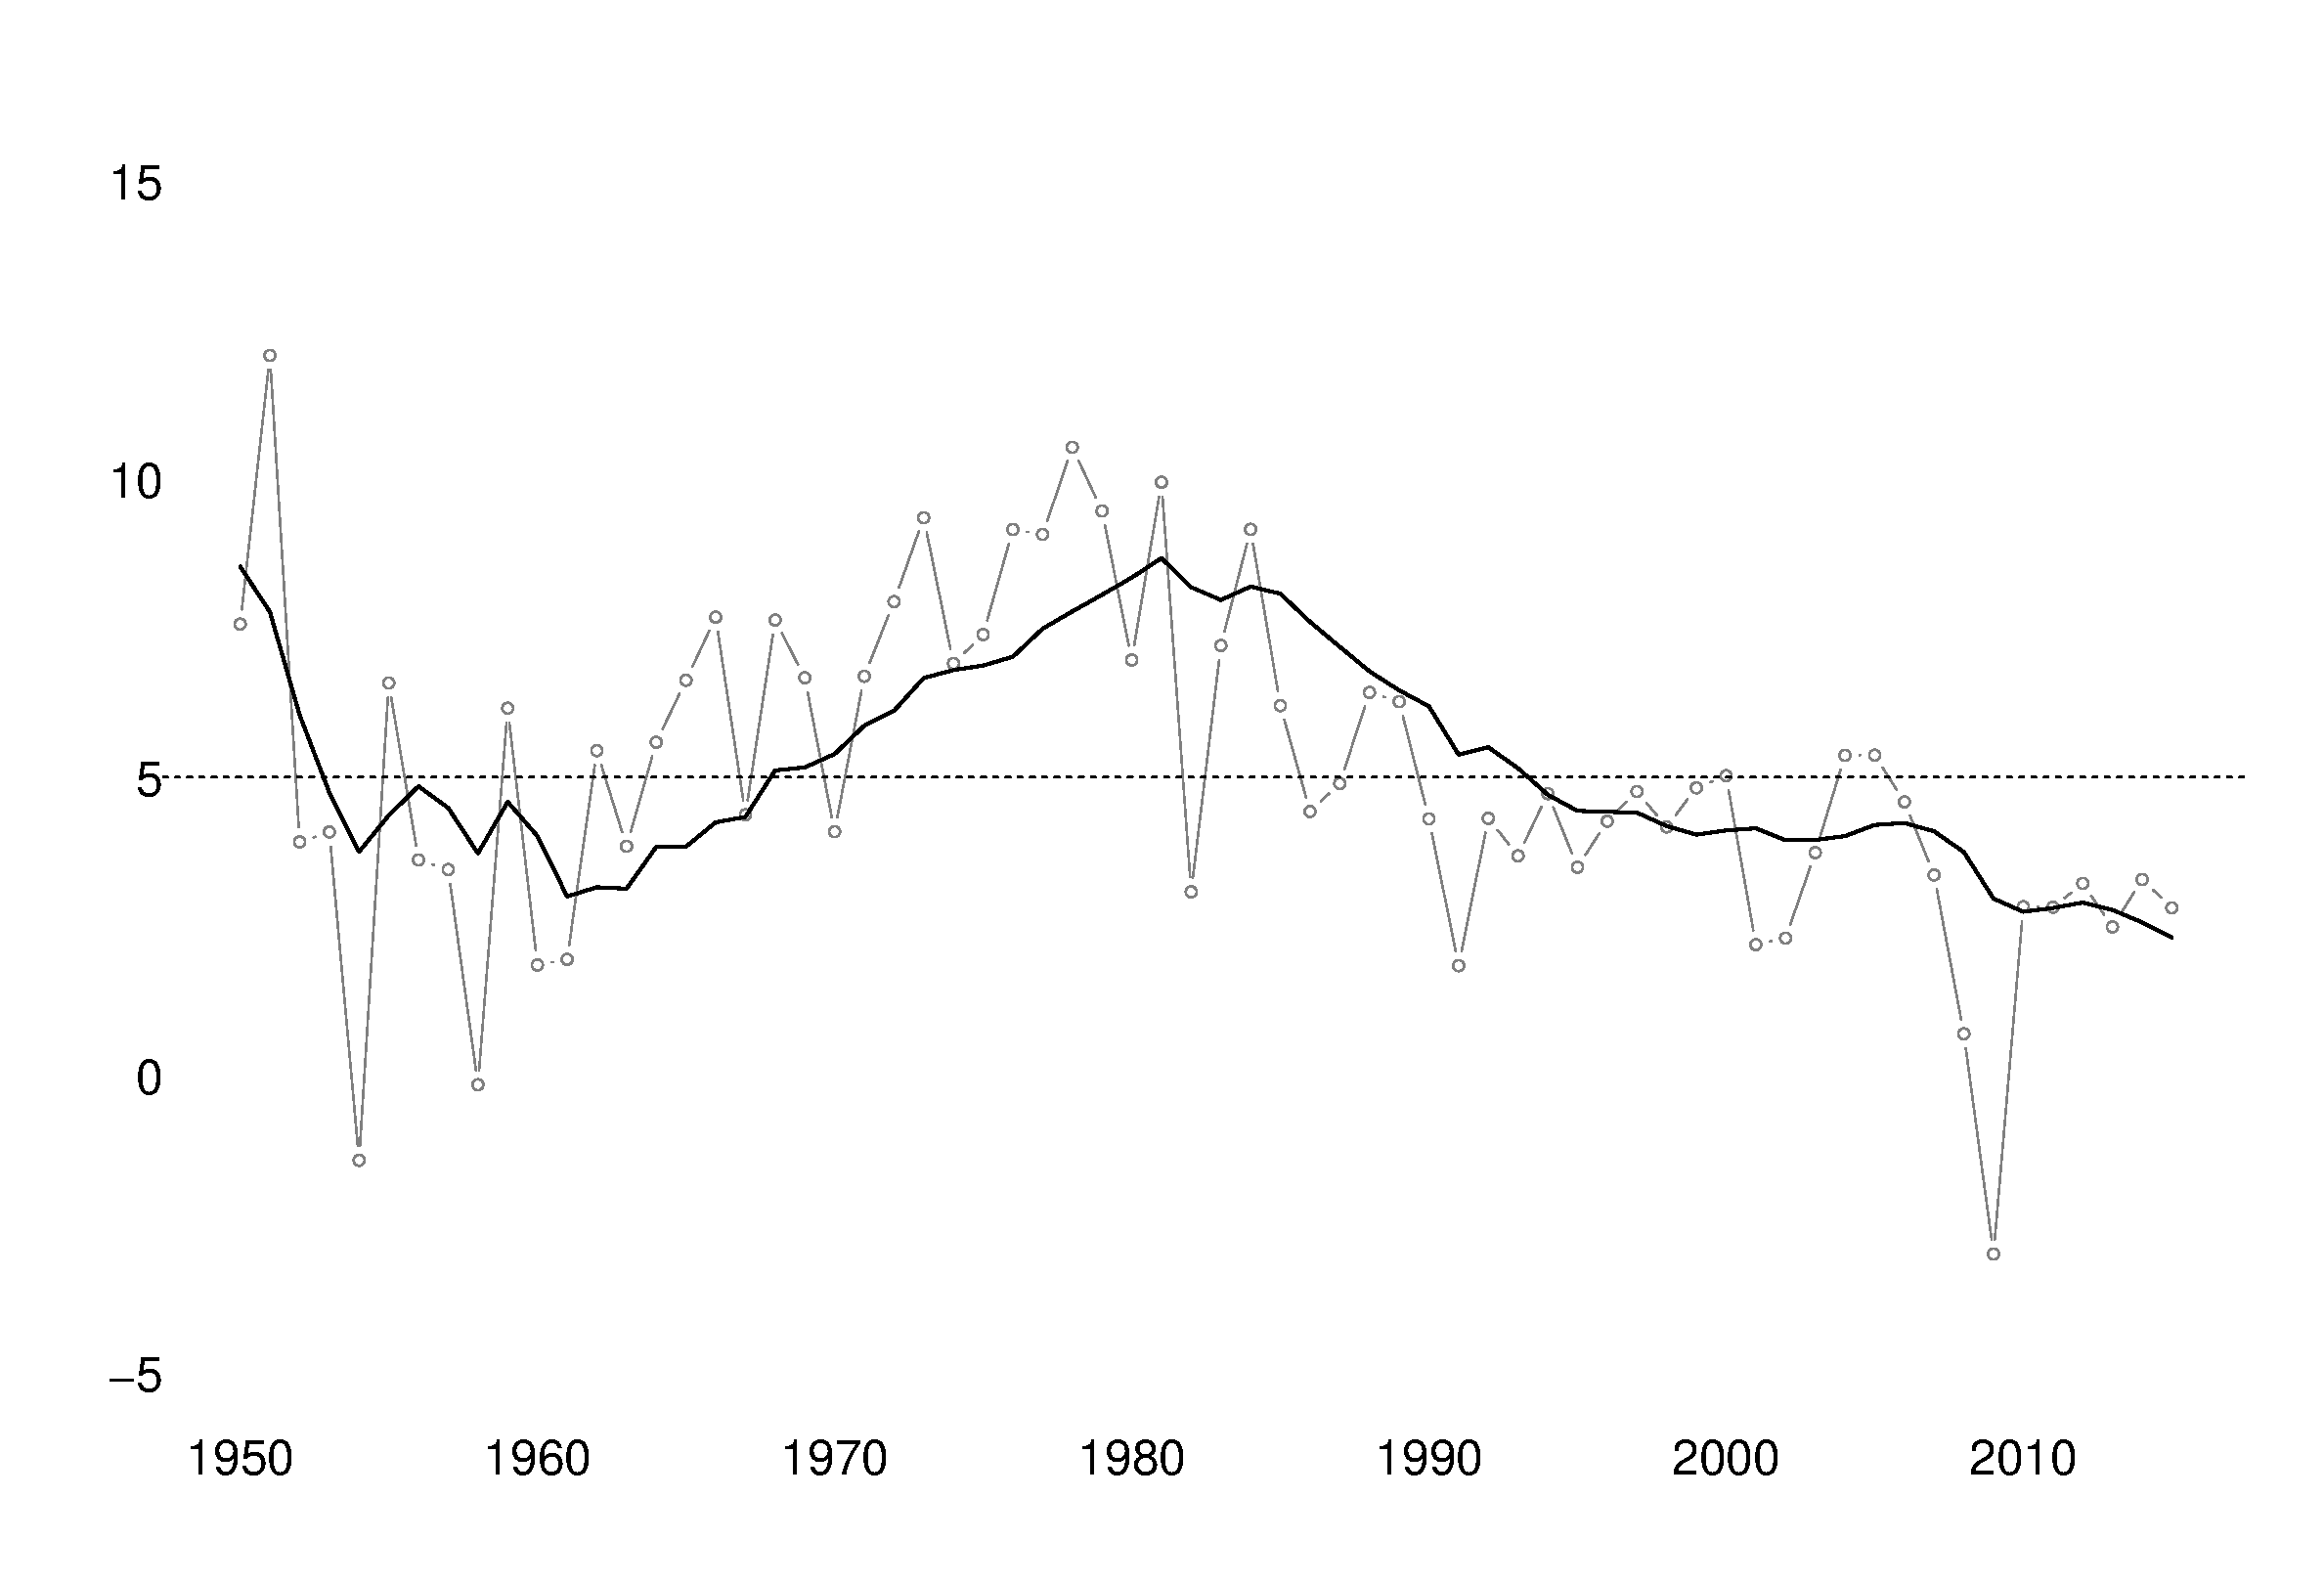
\includegraphics[scale=.3]{us_gdp_g.eps}
  \end{figure}
\end{frame}
%--------------------------------------


%--------------------------------------
\begin{frame}
  Since $\Delta y_t$ is stationary, taking first-differences will remove non-stationary stochastic trend component ($y_{t-1}$) in the data
  \begin{align}
    \Delta y_t= y_t - y_{t-1}=g+\epsilon_t
  \end{align}
  \medskip
  Therefore, fitting a log-linear line to the data, there might appear to be a mean-reverting cyclical component, which is not there.  
\end{frame}
%--------------------------------------


%--------------------------------------
\begin{frame}
  An example: data is randomly generate for following model
  \begin{align}
    y_t=g+y_{t-1}+\epsilon_t
  \end{align}
  \medskip
  $g$=3; starting value for $y$ is 100\\
  $\epsilon \sim N(0,6)$\\
  Take first-differences
  \begin{align}
    \Delta y = y_t - y_{t-1}
  \end{align}
\end{frame}
%--------------------------------------

%--------------------------------------
\begin{frame}
  \begin{figure}
    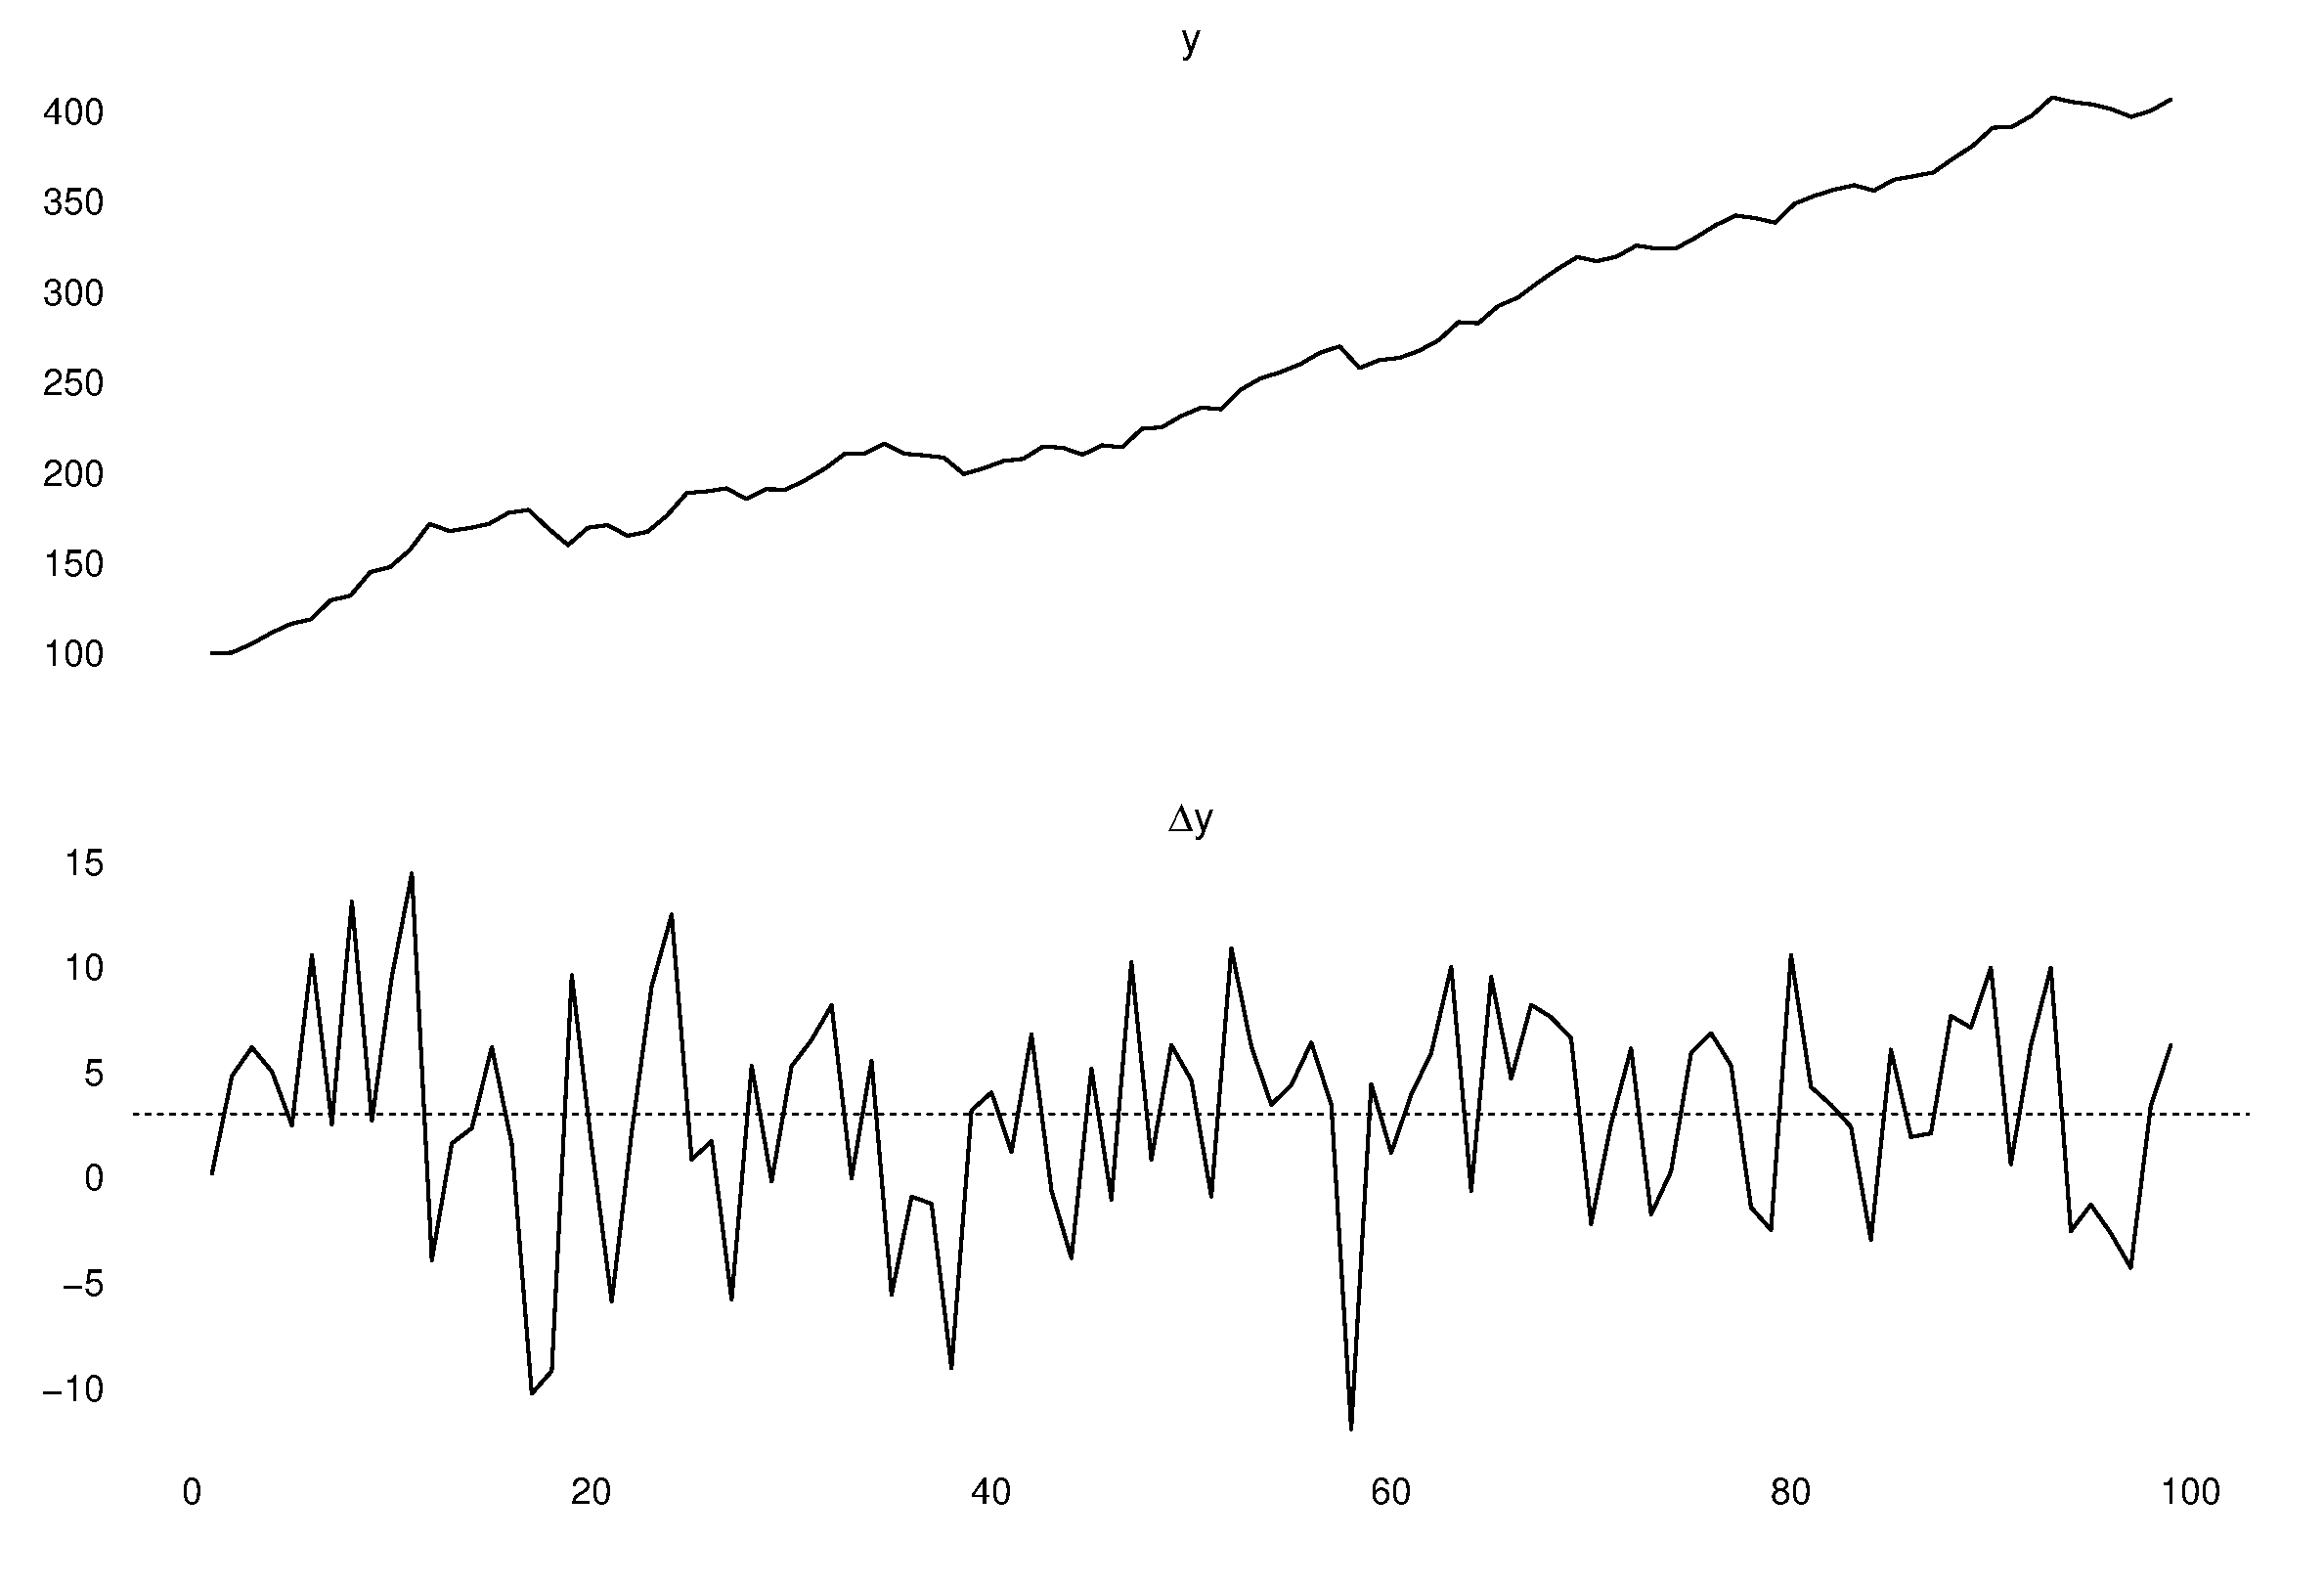
\includegraphics[scale=.3]{detrending_issue.eps}
  \end{figure}
\end{frame}
%--------------------------------------

%--------------------------------------
\begin{frame}
  Incorrect usage of time-series dynamics can lead to errors in identification. 
  An interesting example comes from a paper on the link between precipitation, economic growth, and conflict by Miguel et al. (2004) who use the following IV-2SLS model
  \begin{align}
    \Delta Y_{it} &= a_{1i} + b_1X'_{it} + c_{1,0}\Delta R_{it} + c_{1,1} \Delta R_{it-1} + d_{1i}y_t +\epsilon_{1it}\\
    C_{it} &= \alpha_{2i} + \beta_2 X'_{it} + \gamma_{2,0} \Delta \hat{Y}_{it} + \gamma_{2,1} \Delta \hat{Y}_{it-1} + \delta_{2,1} + \epsilon_{2it}
  \end{align}
  \medskip
  One issue here is that precipitation is mean-reverting.
\end{frame}
%--------------------------------------


%--------------------------------------
\begin{frame}
  Ciccone (2011) argues the following; consider the following model to link conflict and precipitation   
  \begin{align}
    P(conflict_t) &= a \Delta R_t + b \Delta R_{t-1}  
  \end{align}
  \medskip
  Can write this in levels as
  \begin{align}
    P(conflict_t) &= \alpha_0\log\; R_t + \alpha_1 log\; R_{t-1} + \alpha_2 log\; R_{t-2}  
  \end{align}    
\end{frame}
%--------------------------------------

%--------------------------------------
\begin{frame}
Given that 
  \begin{align}
    \Delta R_t = log\;R_t - log\; R_{t-1}
  \end{align}
  \medskip 
  The estimates in Eq.12 are given by
  \begin{align}
    a=\frac{2\alpha_0-(\alpha_1+\alpha_2)}{3}; b=\frac{(\alpha_0 + \alpha_1)-2\alpha_2}{3}
  \end{align}
  \medskip
  i.e. parameters in eq.12 are a mixture of those in eq.13.
\end{frame}
%--------------------------------------

%--------------------------------------
\begin{frame}
 A commonly use method to detrend data is the Hodrick-Prescott (HP) filter; taking $y_t$ the filter minimises
\begin{align}
 \sum_{t=1}^{N} [(y_t - y_t^*)^2+ \lambda(\Delta y_t^* - \Delta y_{t-1}^*)]
\end{align}
\medskip
Here $y^*$ is the time-varying trend; $\lambda$ is a penalty parameter
\begin{itemize}
  \item For quarterly data $\lambda=1,600$
\end{itemize}
\end{frame}
%--------------------------------------

%--------------------------------------
\begin{frame}
  The HP filter does two things:
  \begin{enumerate}
    \item Minimise the sum of squared deviations between output and its trend
    \begin{align}
      (Y_t - Y_t^*)^2
    \end{align}
    \item Minimising the change in the trend growth rate
    \begin{align}
      \lambda(\Delta Y_t^* - \Delta Y_{t-1}^*)
    \end{align}
  \end{enumerate}
  \medskip
  Important is that the HP-filter let's the growth rate very over time.
  \begin{itemize}
    \item Larger $\lambda$ means smoother trend
  \end{itemize}
\end{frame}
%--------------------------------------

%--------------------------------------
\begin{frame}
  \begin{figure}
    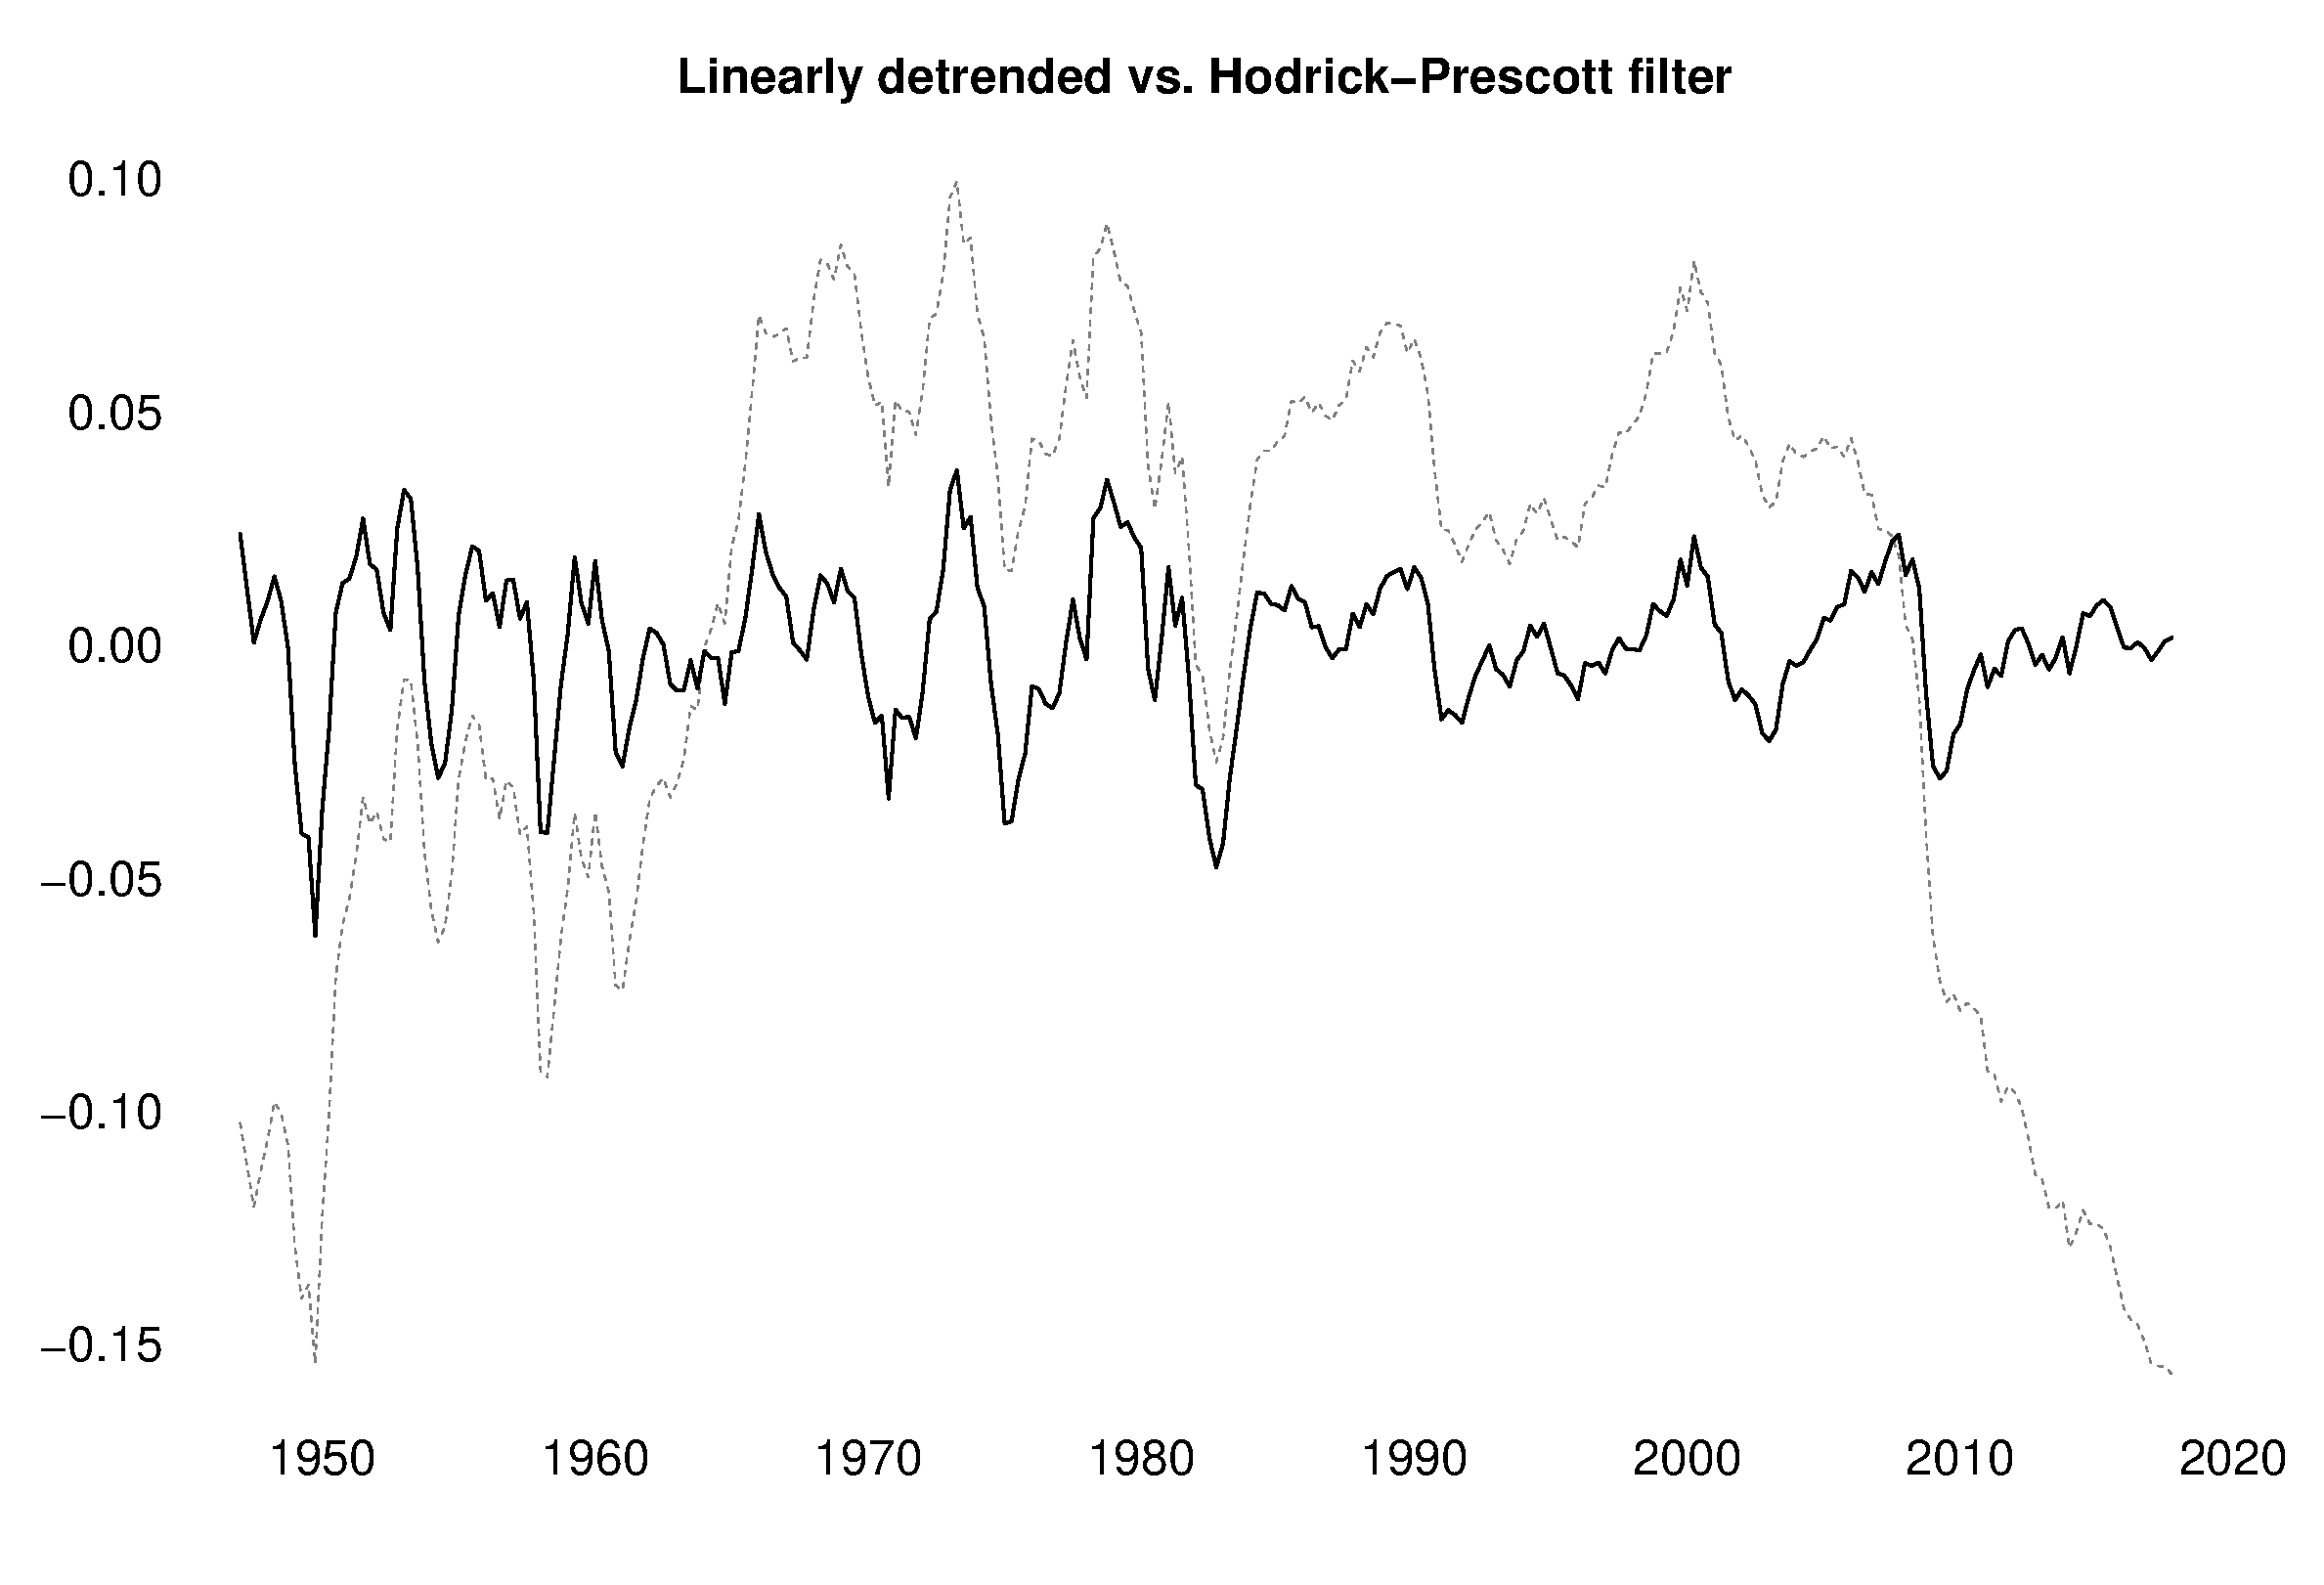
\includegraphics[scale=.3]{hp_filter.eps}
  \end{figure}
\end{frame}
%--------------------------------------

%--------------------------------------
\begin{frame}
  \begin{figure}
    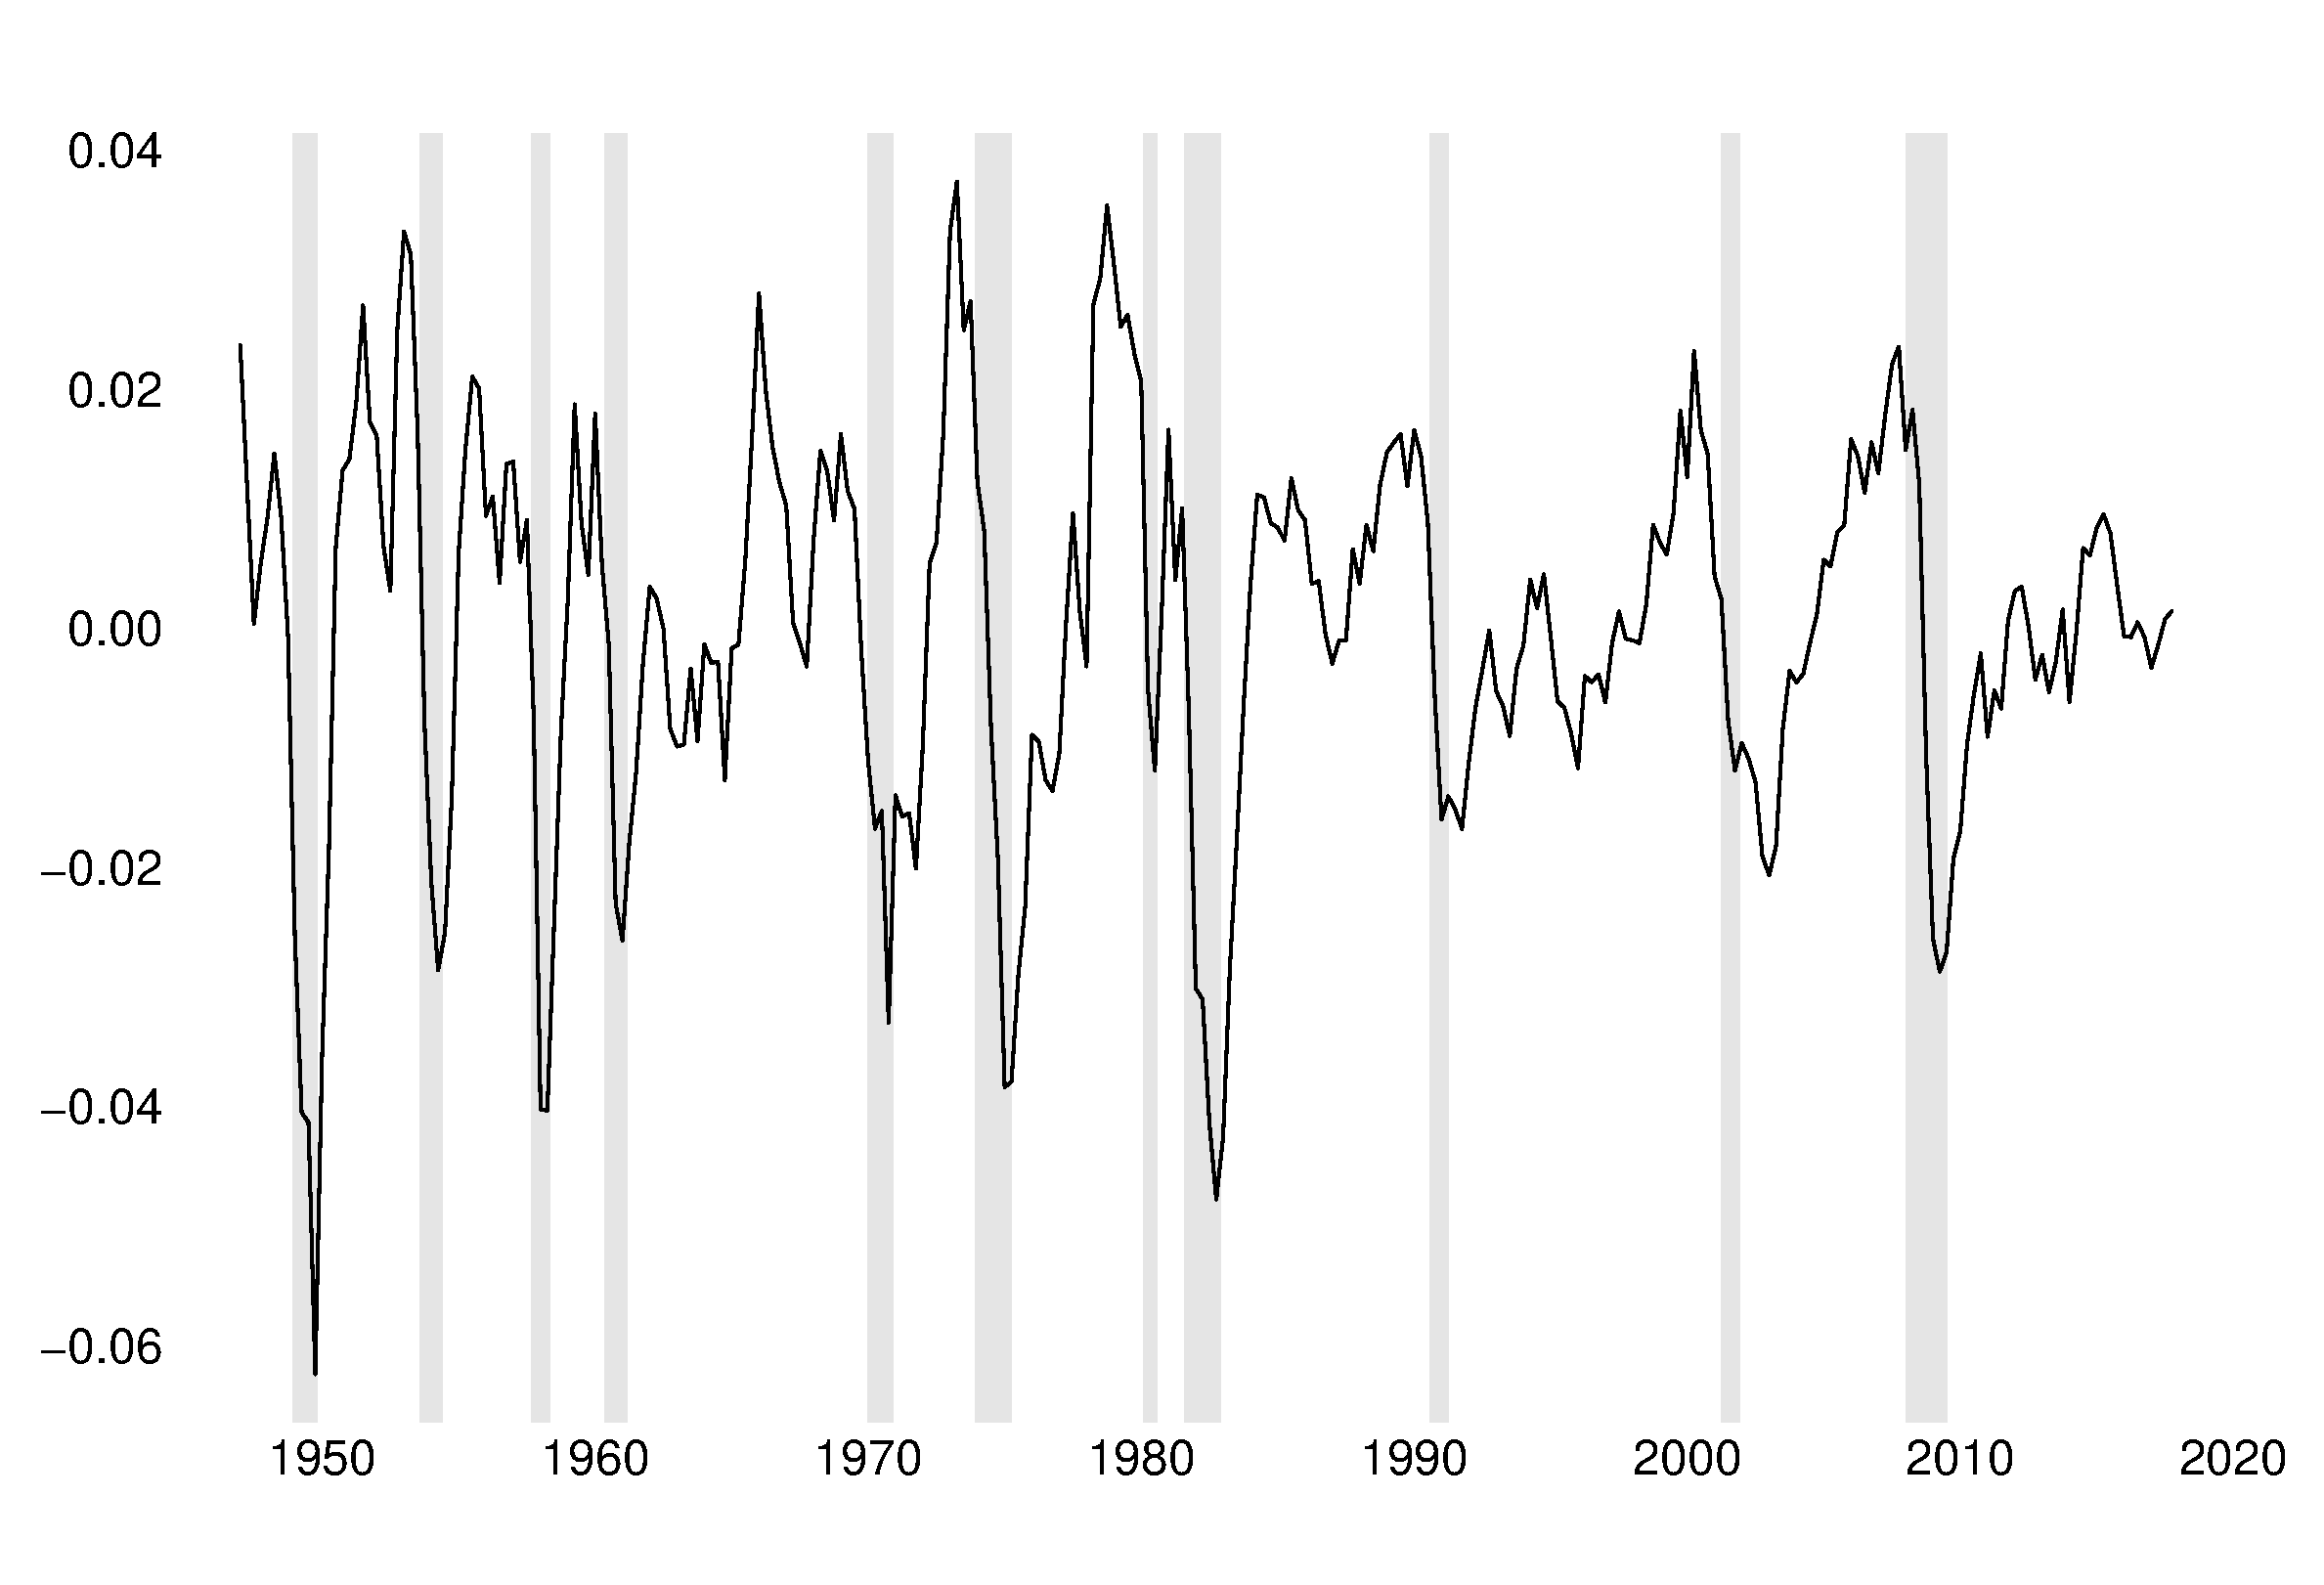
\includegraphics[scale=.3]{hp_filter2.eps}
  \end{figure}
\end{frame}
%--------------------------------------

%--------------------------------------
\begin{frame}
  \begin{figure}
    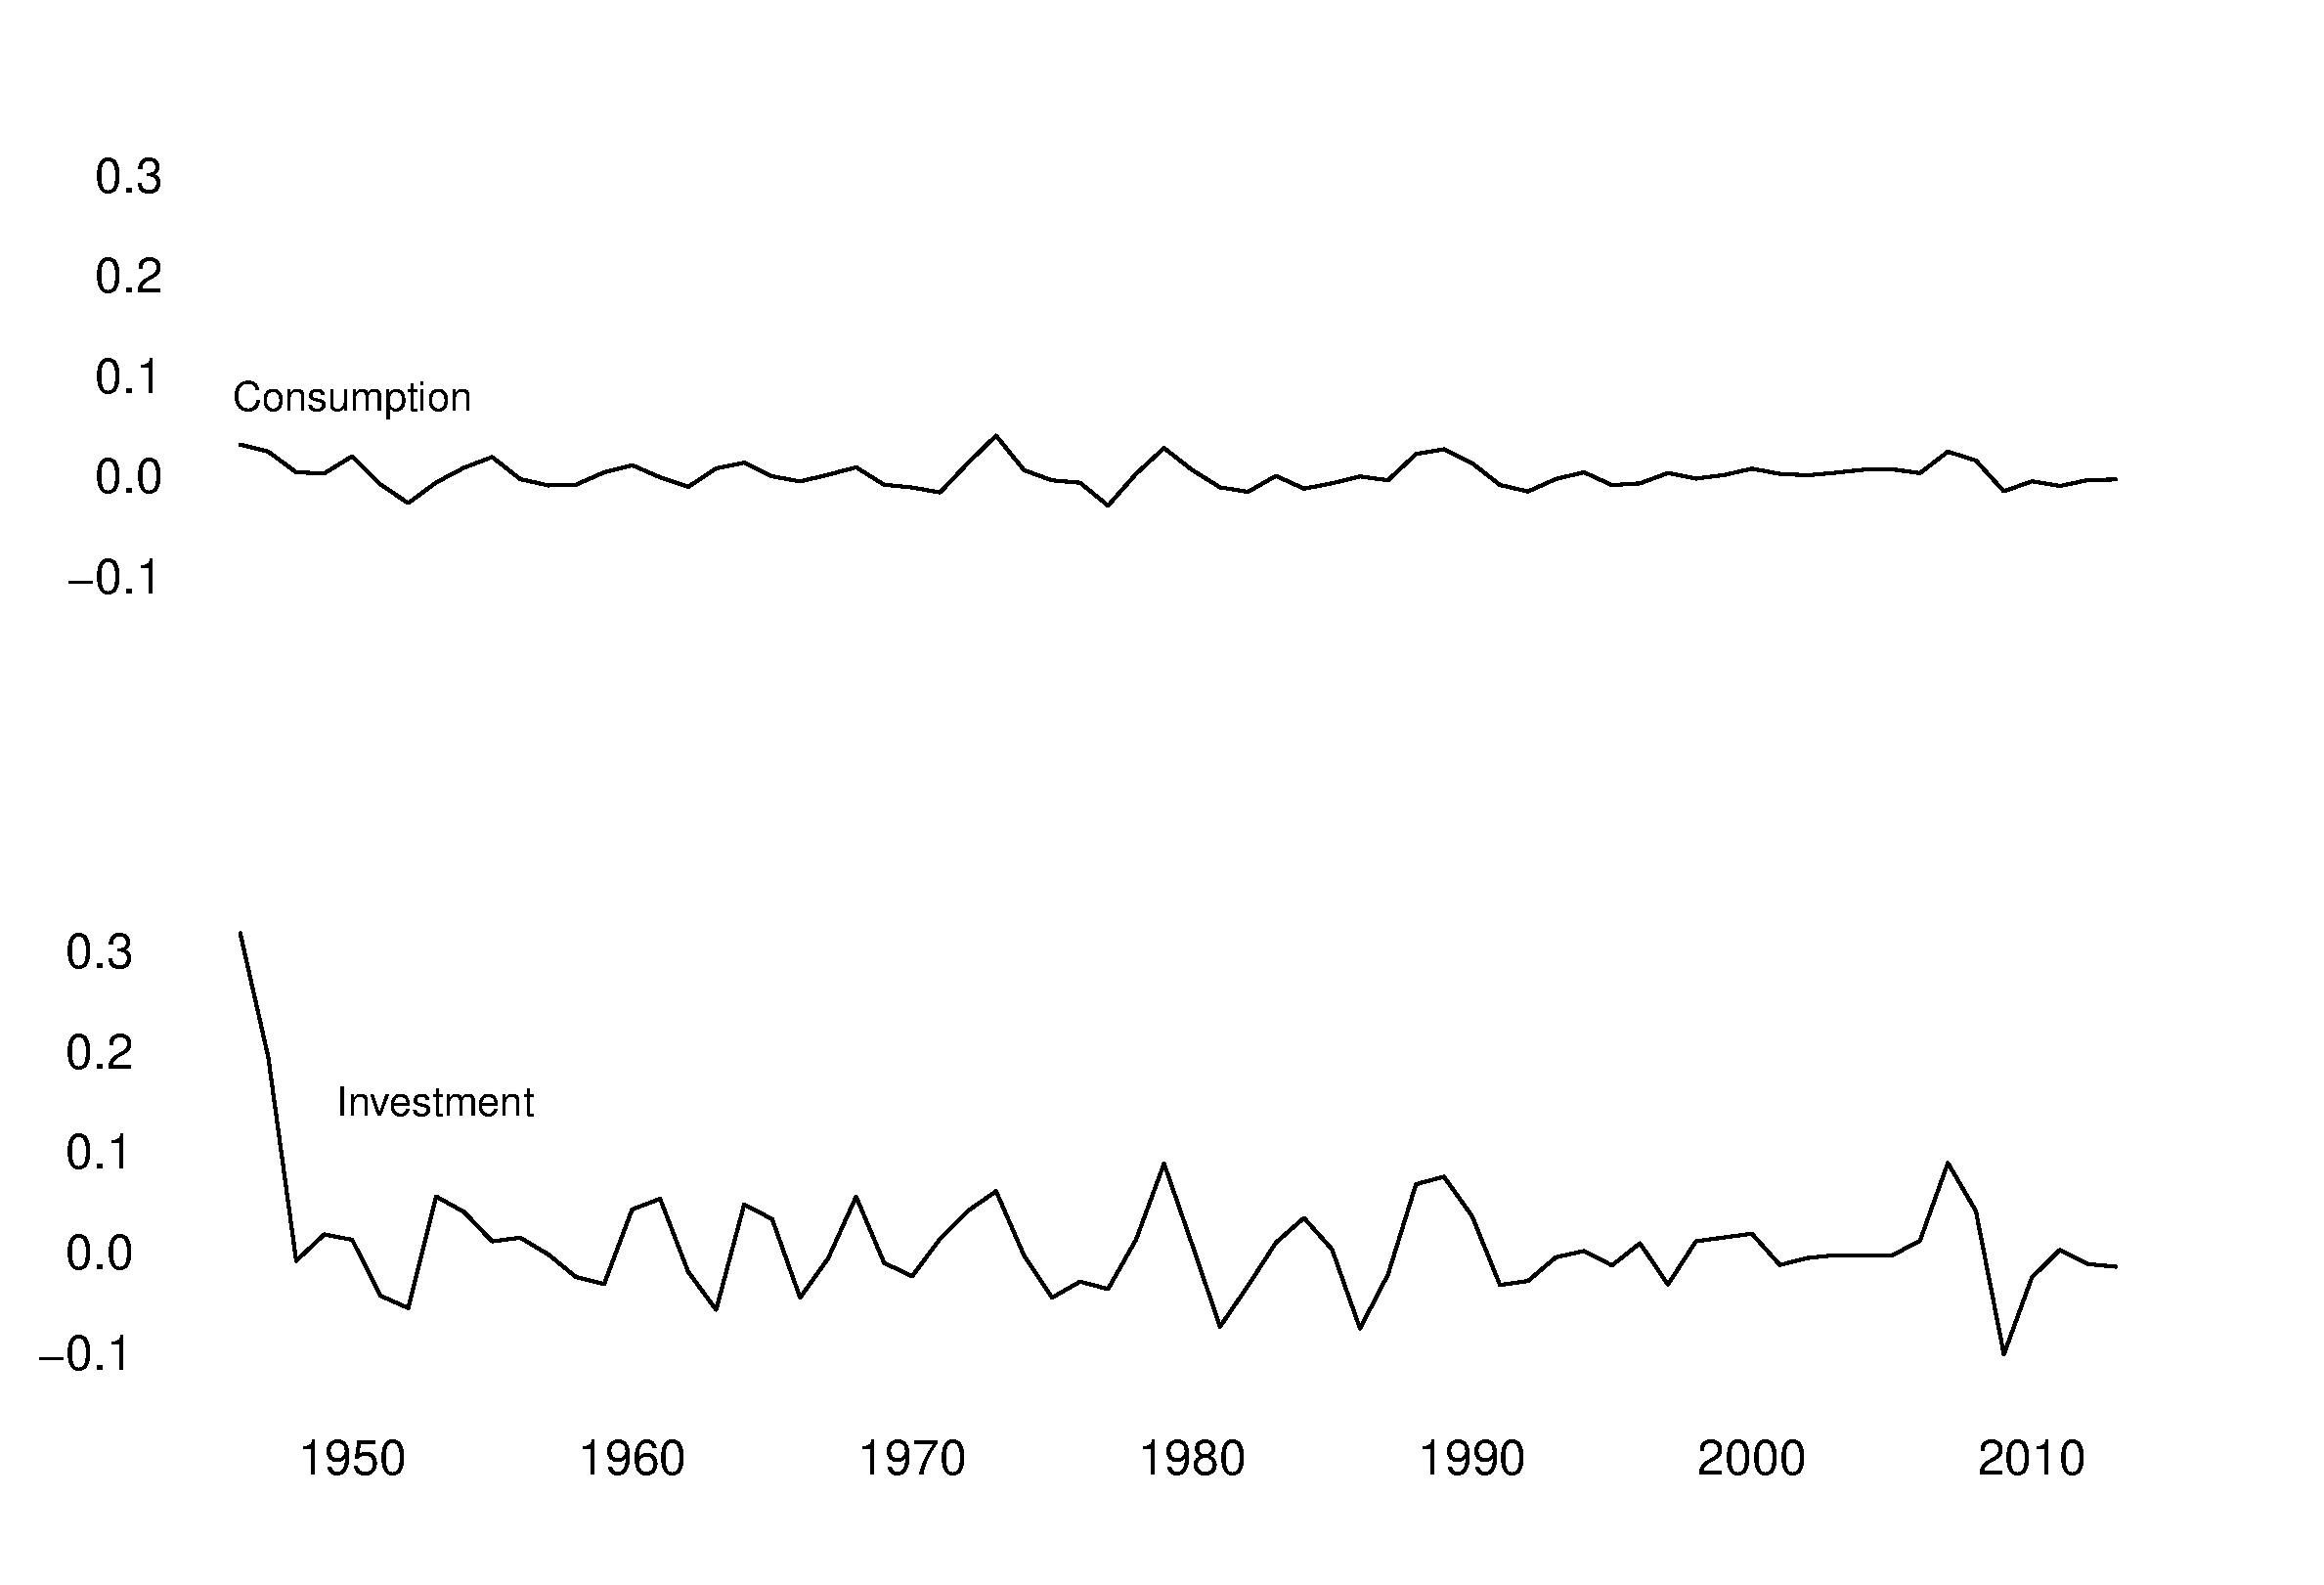
\includegraphics[scale=.3]{uk_ci.eps}
  \end{figure}
\end{frame}
%--------------------------------------

%--------------------------------------
\begin{frame}
  Can use the HP-filter to look at cycles in different components of GDP (this case UK): shows that consumption tends to be more stable
  \begin{enumerate}
    \item The consumption of specifically non-durable goods such as food is stable over time
    \item People tend to spend a constant amount of money regardless of temporary shocks (permanent income hypothesis)
  \end{enumerate}
\end{frame}
%--------------------------------------

%--------------------------------------
\begin{frame}
  \begin{figure}
    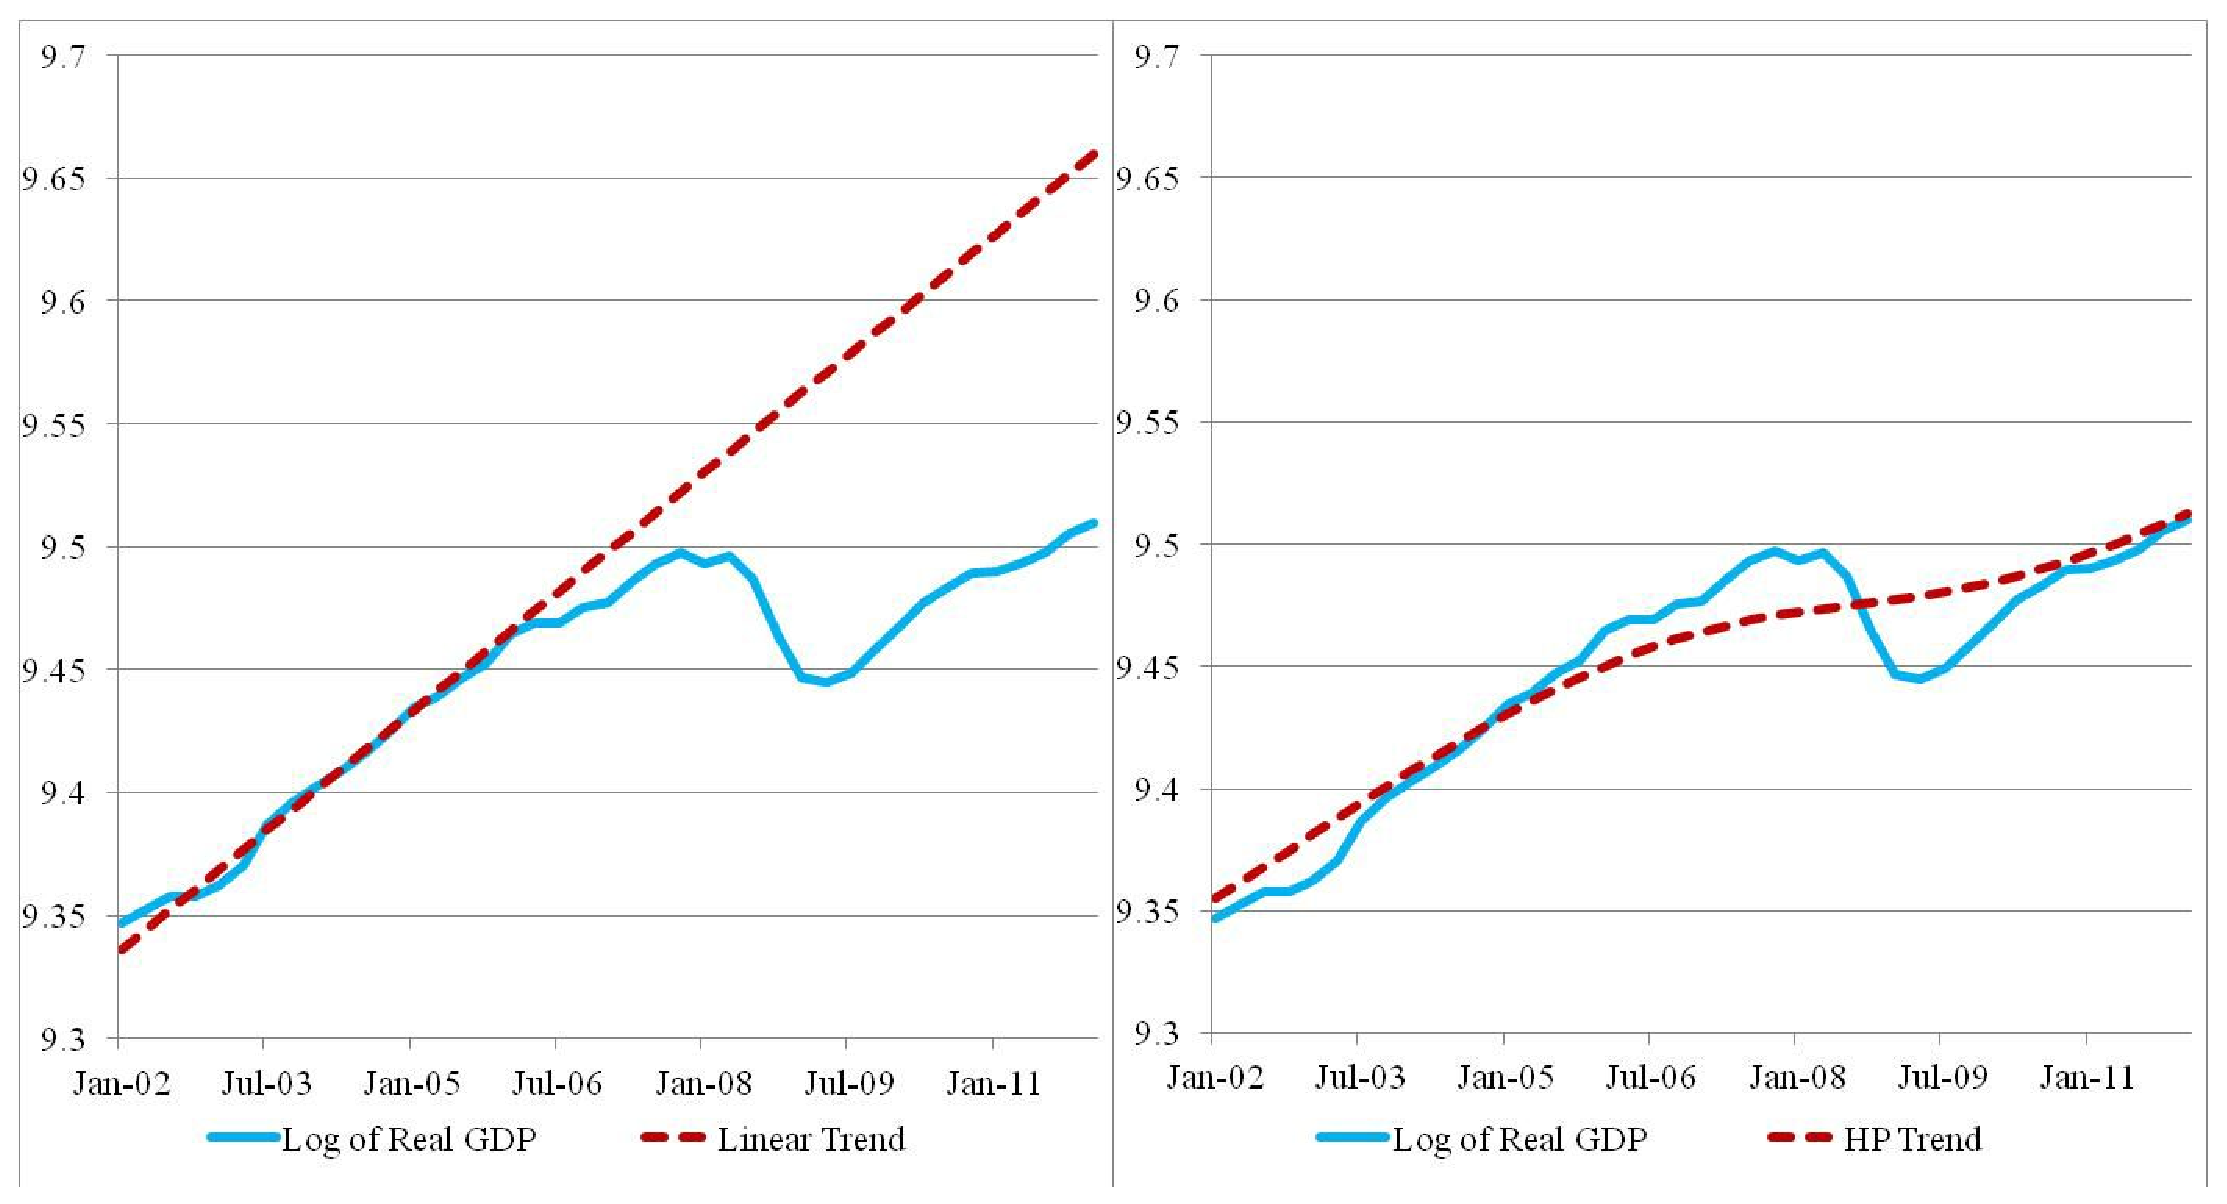
\includegraphics[scale=.3]{us_potential.eps}
  \end{figure}
  Source: James Bullard
\end{frame}
%--------------------------------------

%--------------------------------------
\begin{frame}
  Statistical technique is only useful if assumptions reflect economic reality.
  But HP-filter assumes that deviations from trend are short term and correct themselves quickly
  \begin{itemize}
    \item Prolonged periods below potential GDP not possible
  \end{itemize}
  \medskip
  There is an endpoint problem in the filter
  \begin{itemize}
    \item Smoothed series close to observed data at beginning and end or period
  \end{itemize}  
\end{frame}
%--------------------------------------

%--------------------------------------
\begin{frame}
  \begin{figure}
     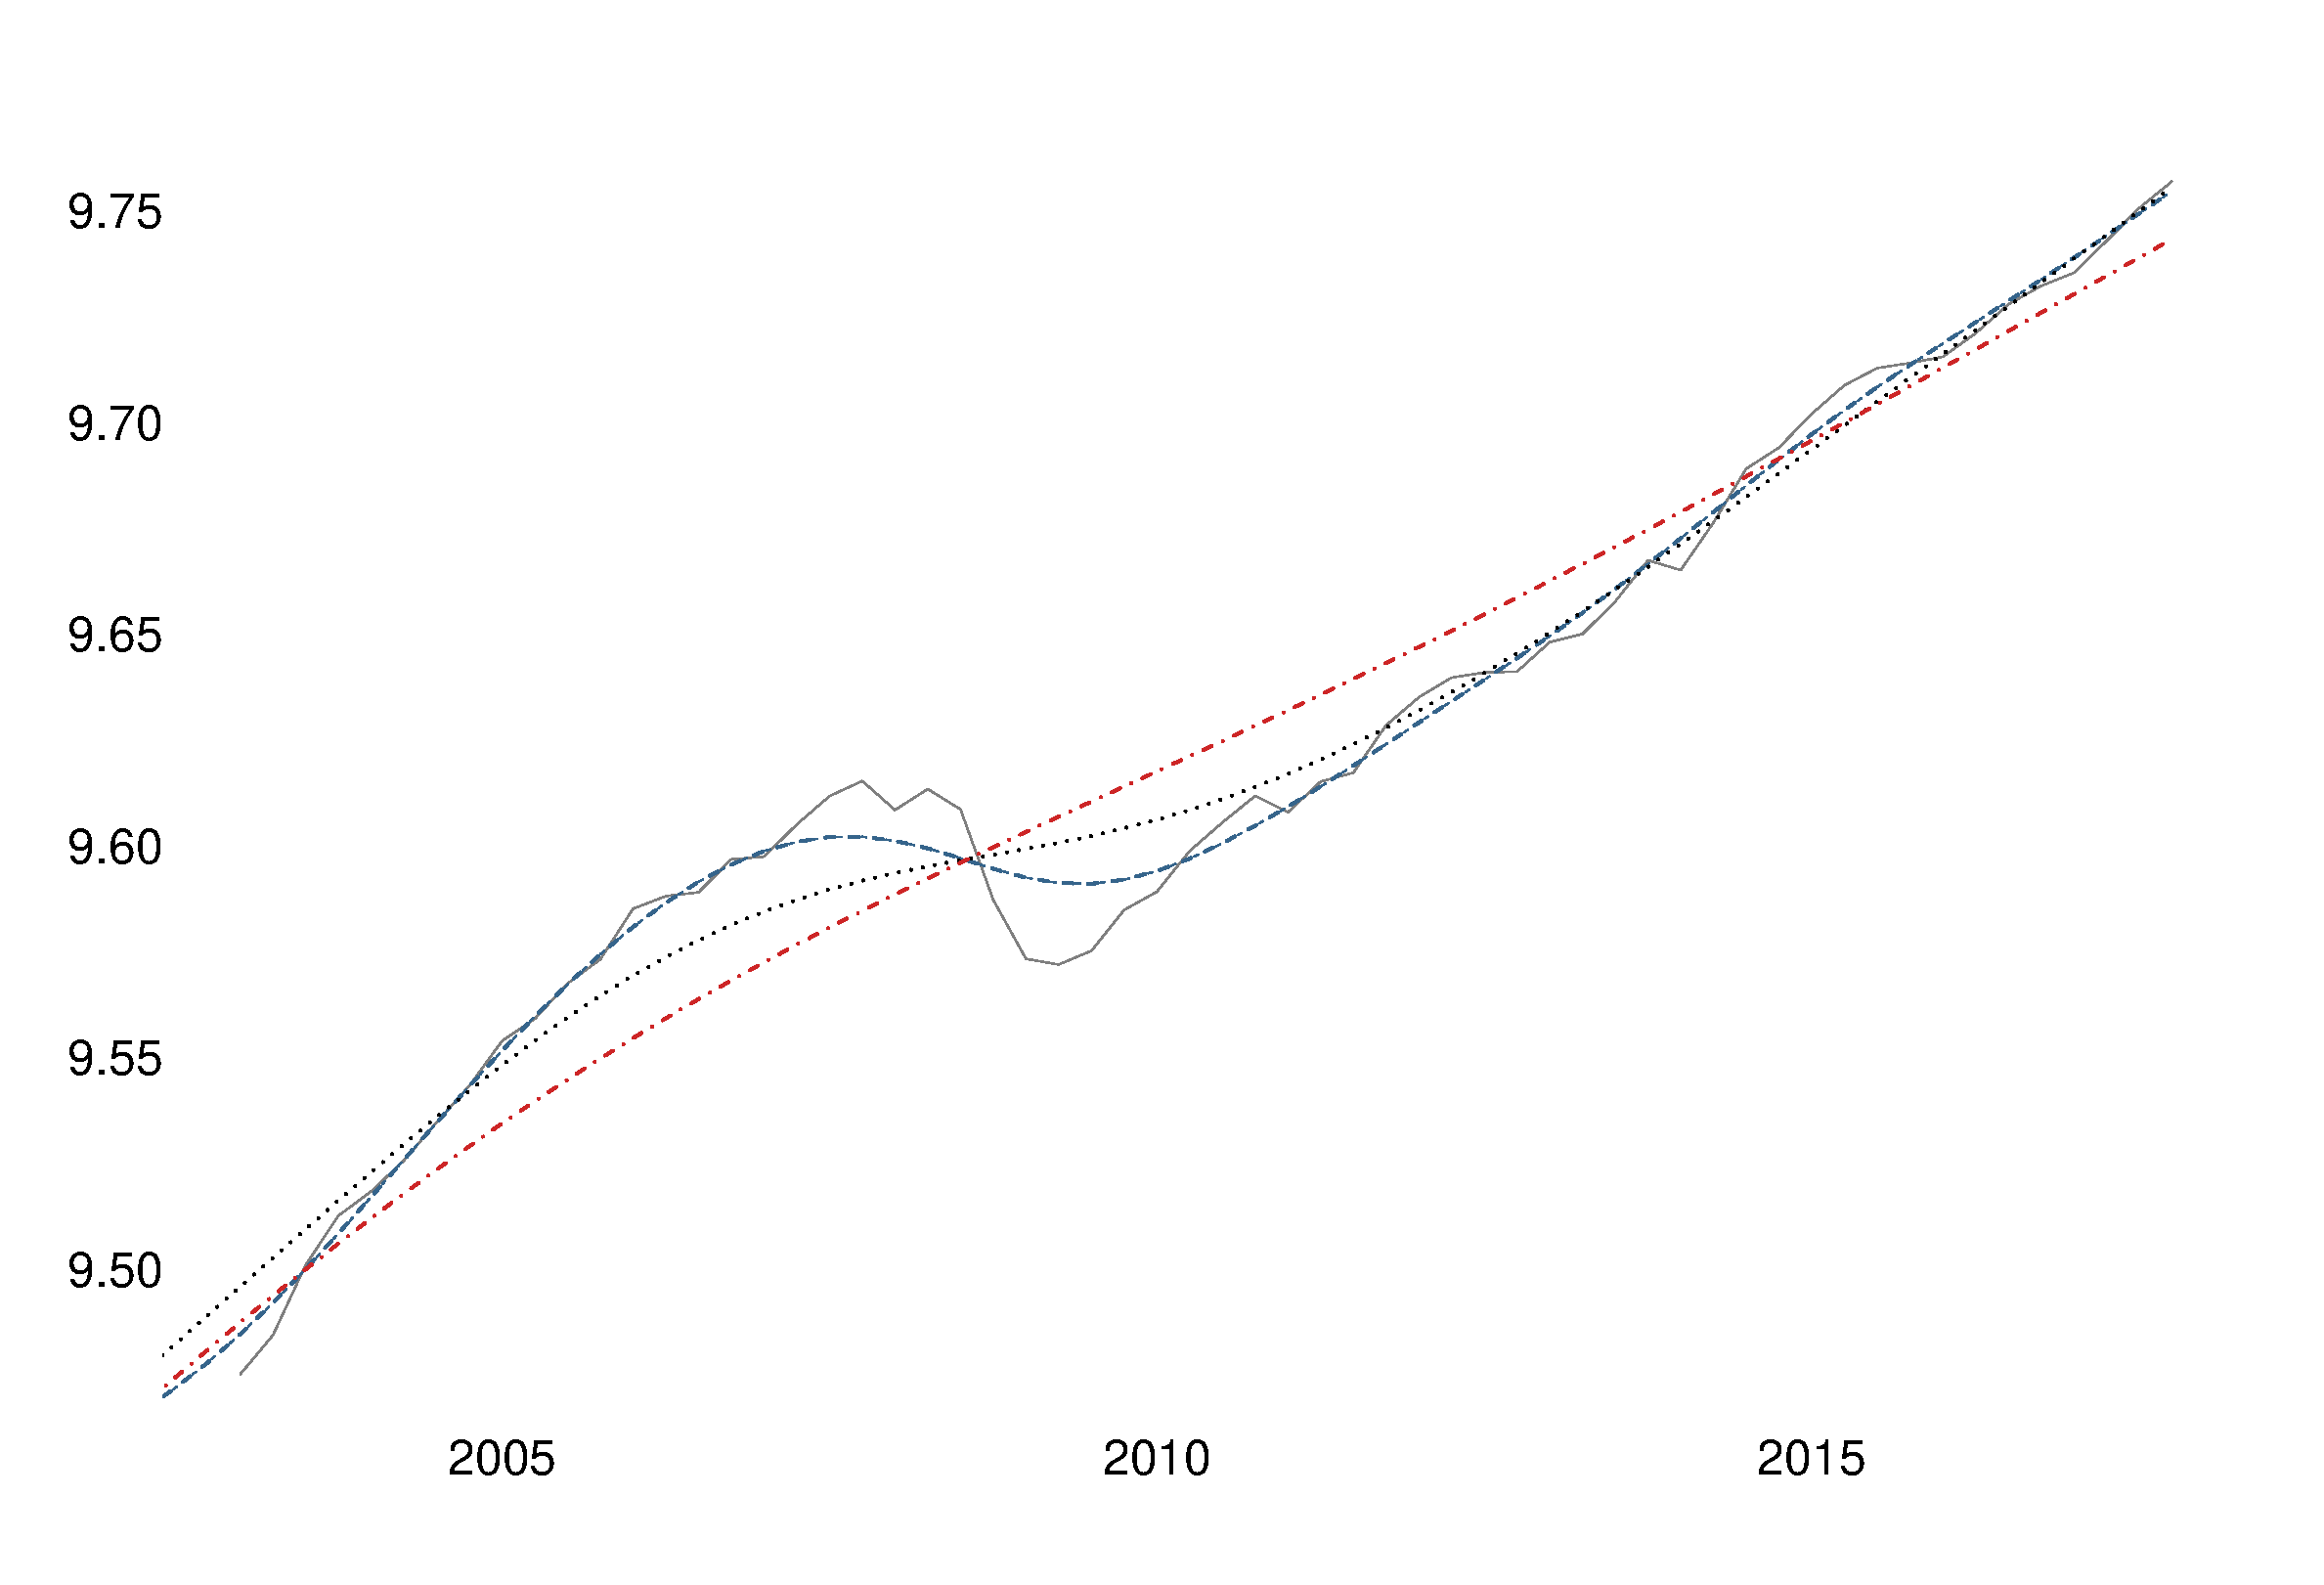
\includegraphics[scale=.3]{hp_lambda.eps}
  \end{figure}
\end{frame}
%--------------------------------------

%--------------------------------------
\begin{frame}
  \begin{figure}
    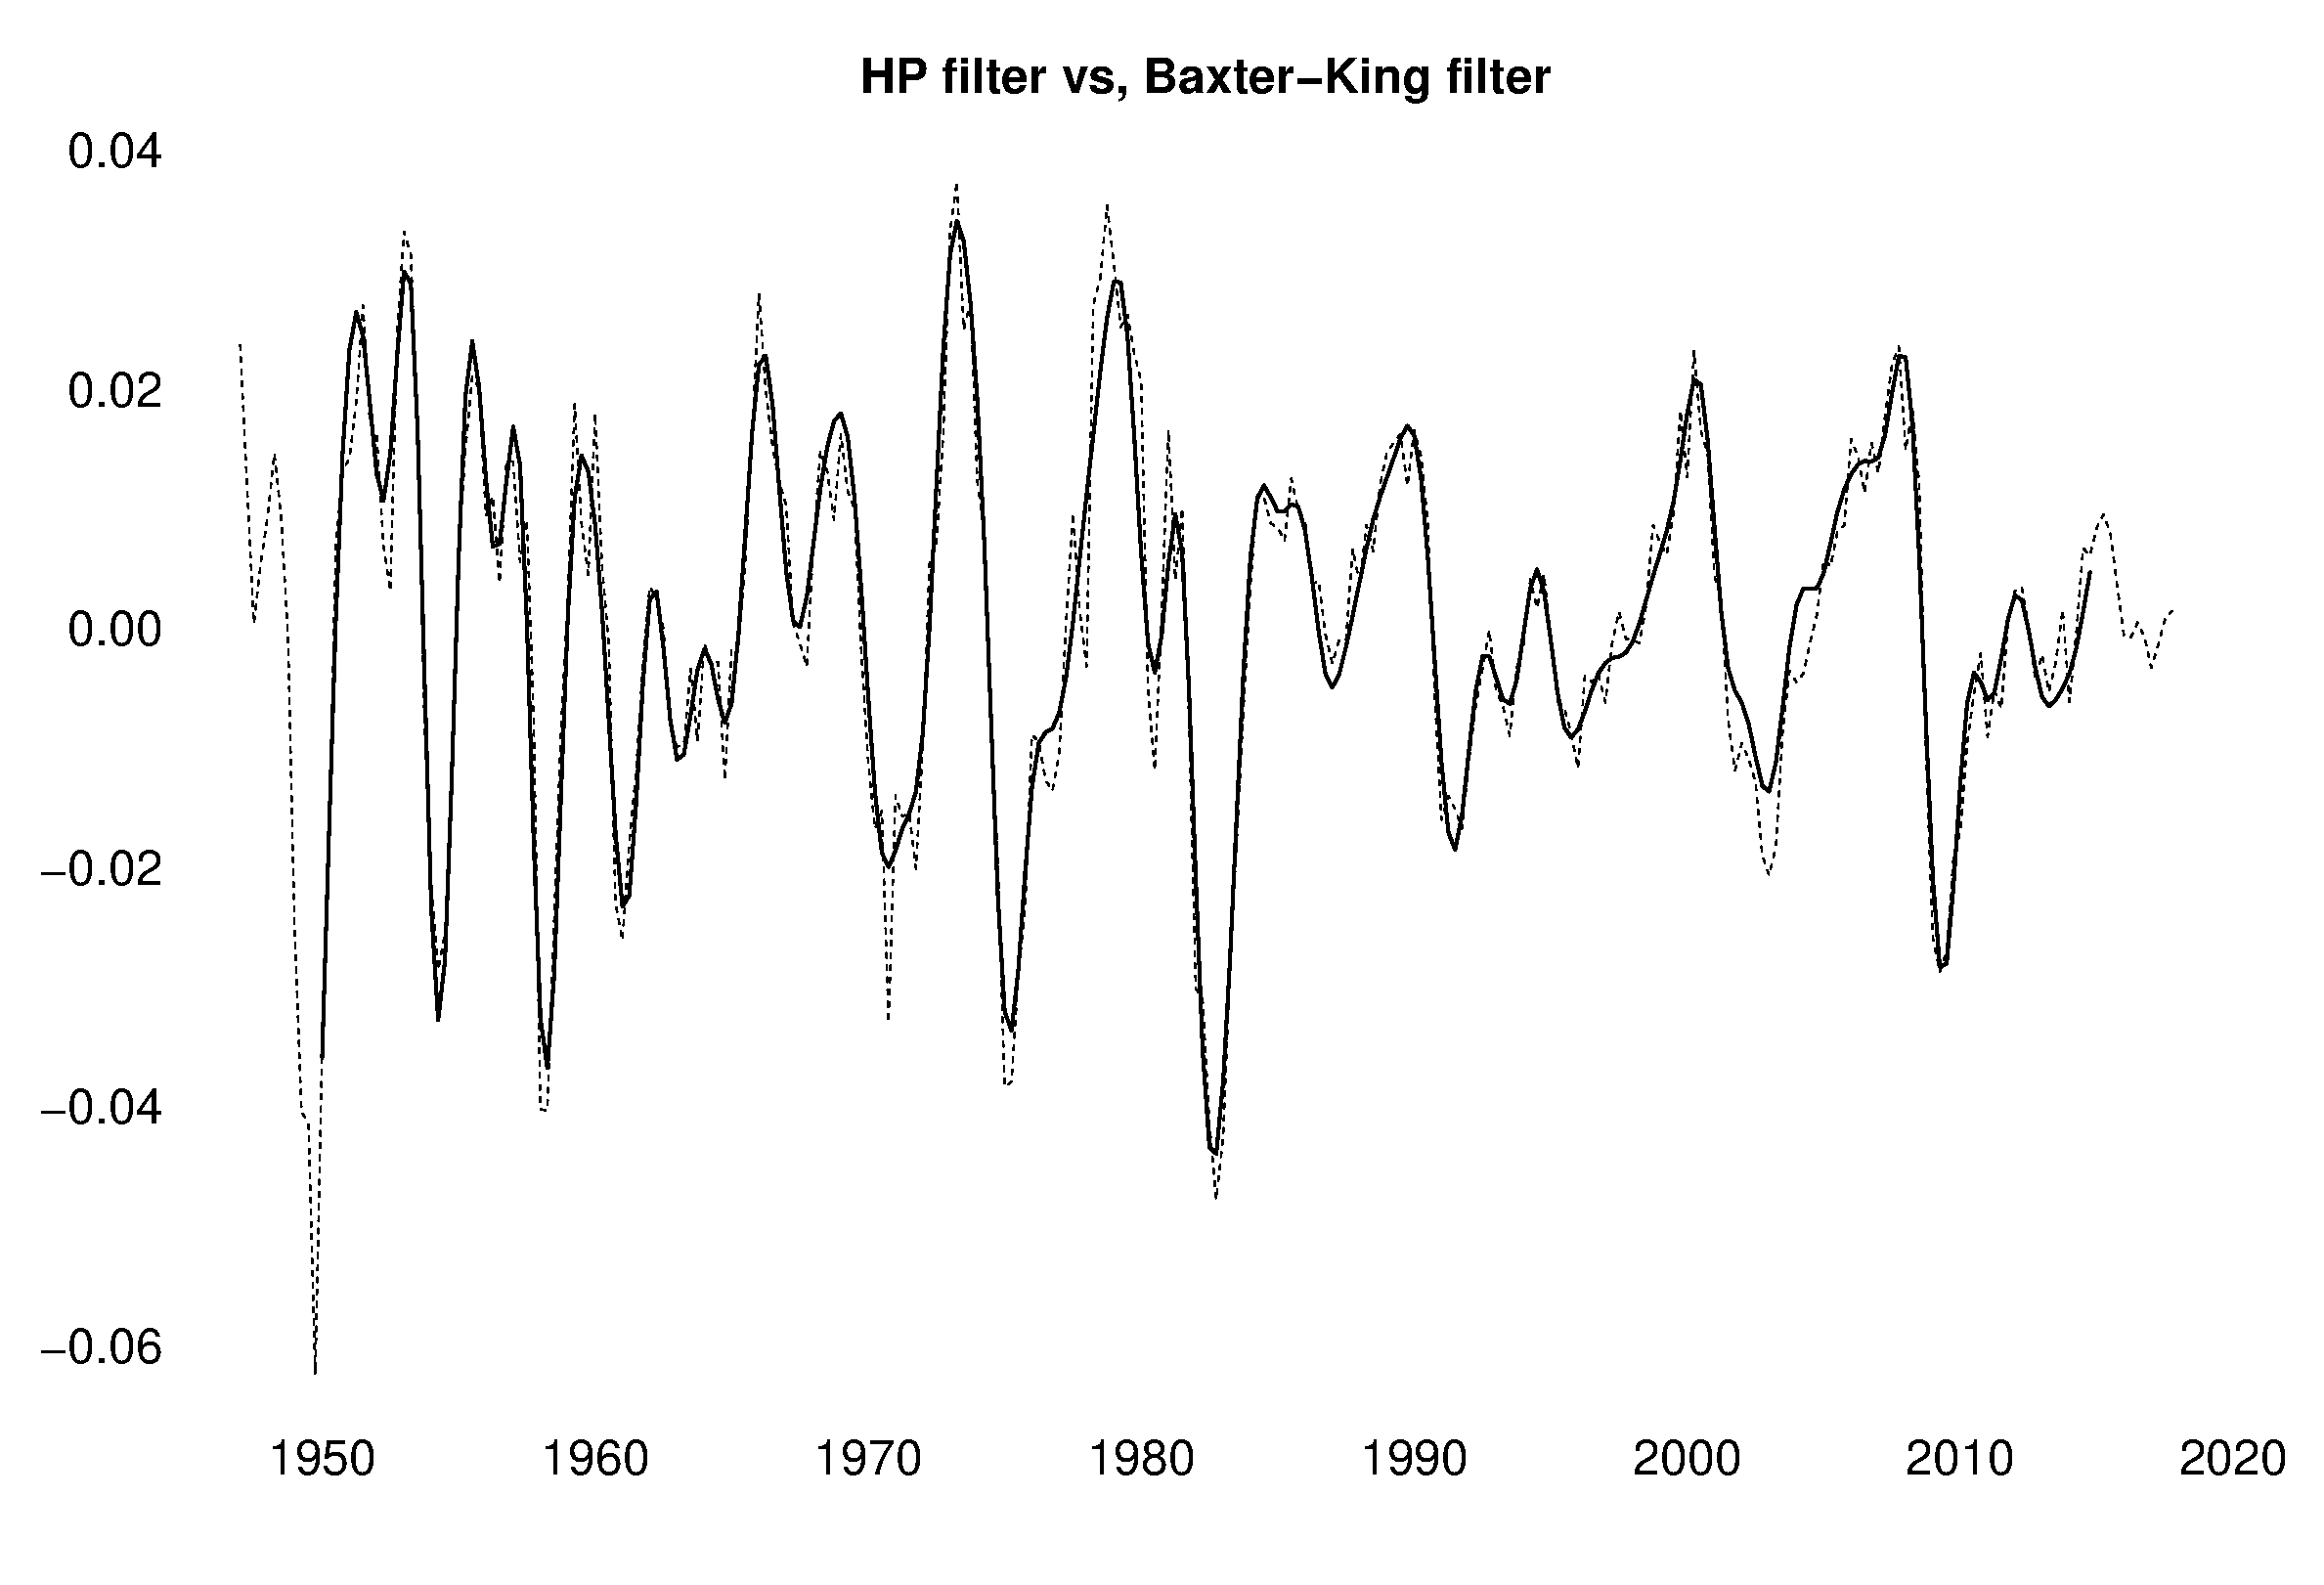
\includegraphics[scale=.3]{baxter_king.eps}
  \end{figure}
\end{frame}
%--------------------------------------


%--------------------------------------
\begin{frame}
  \begin{figure}
    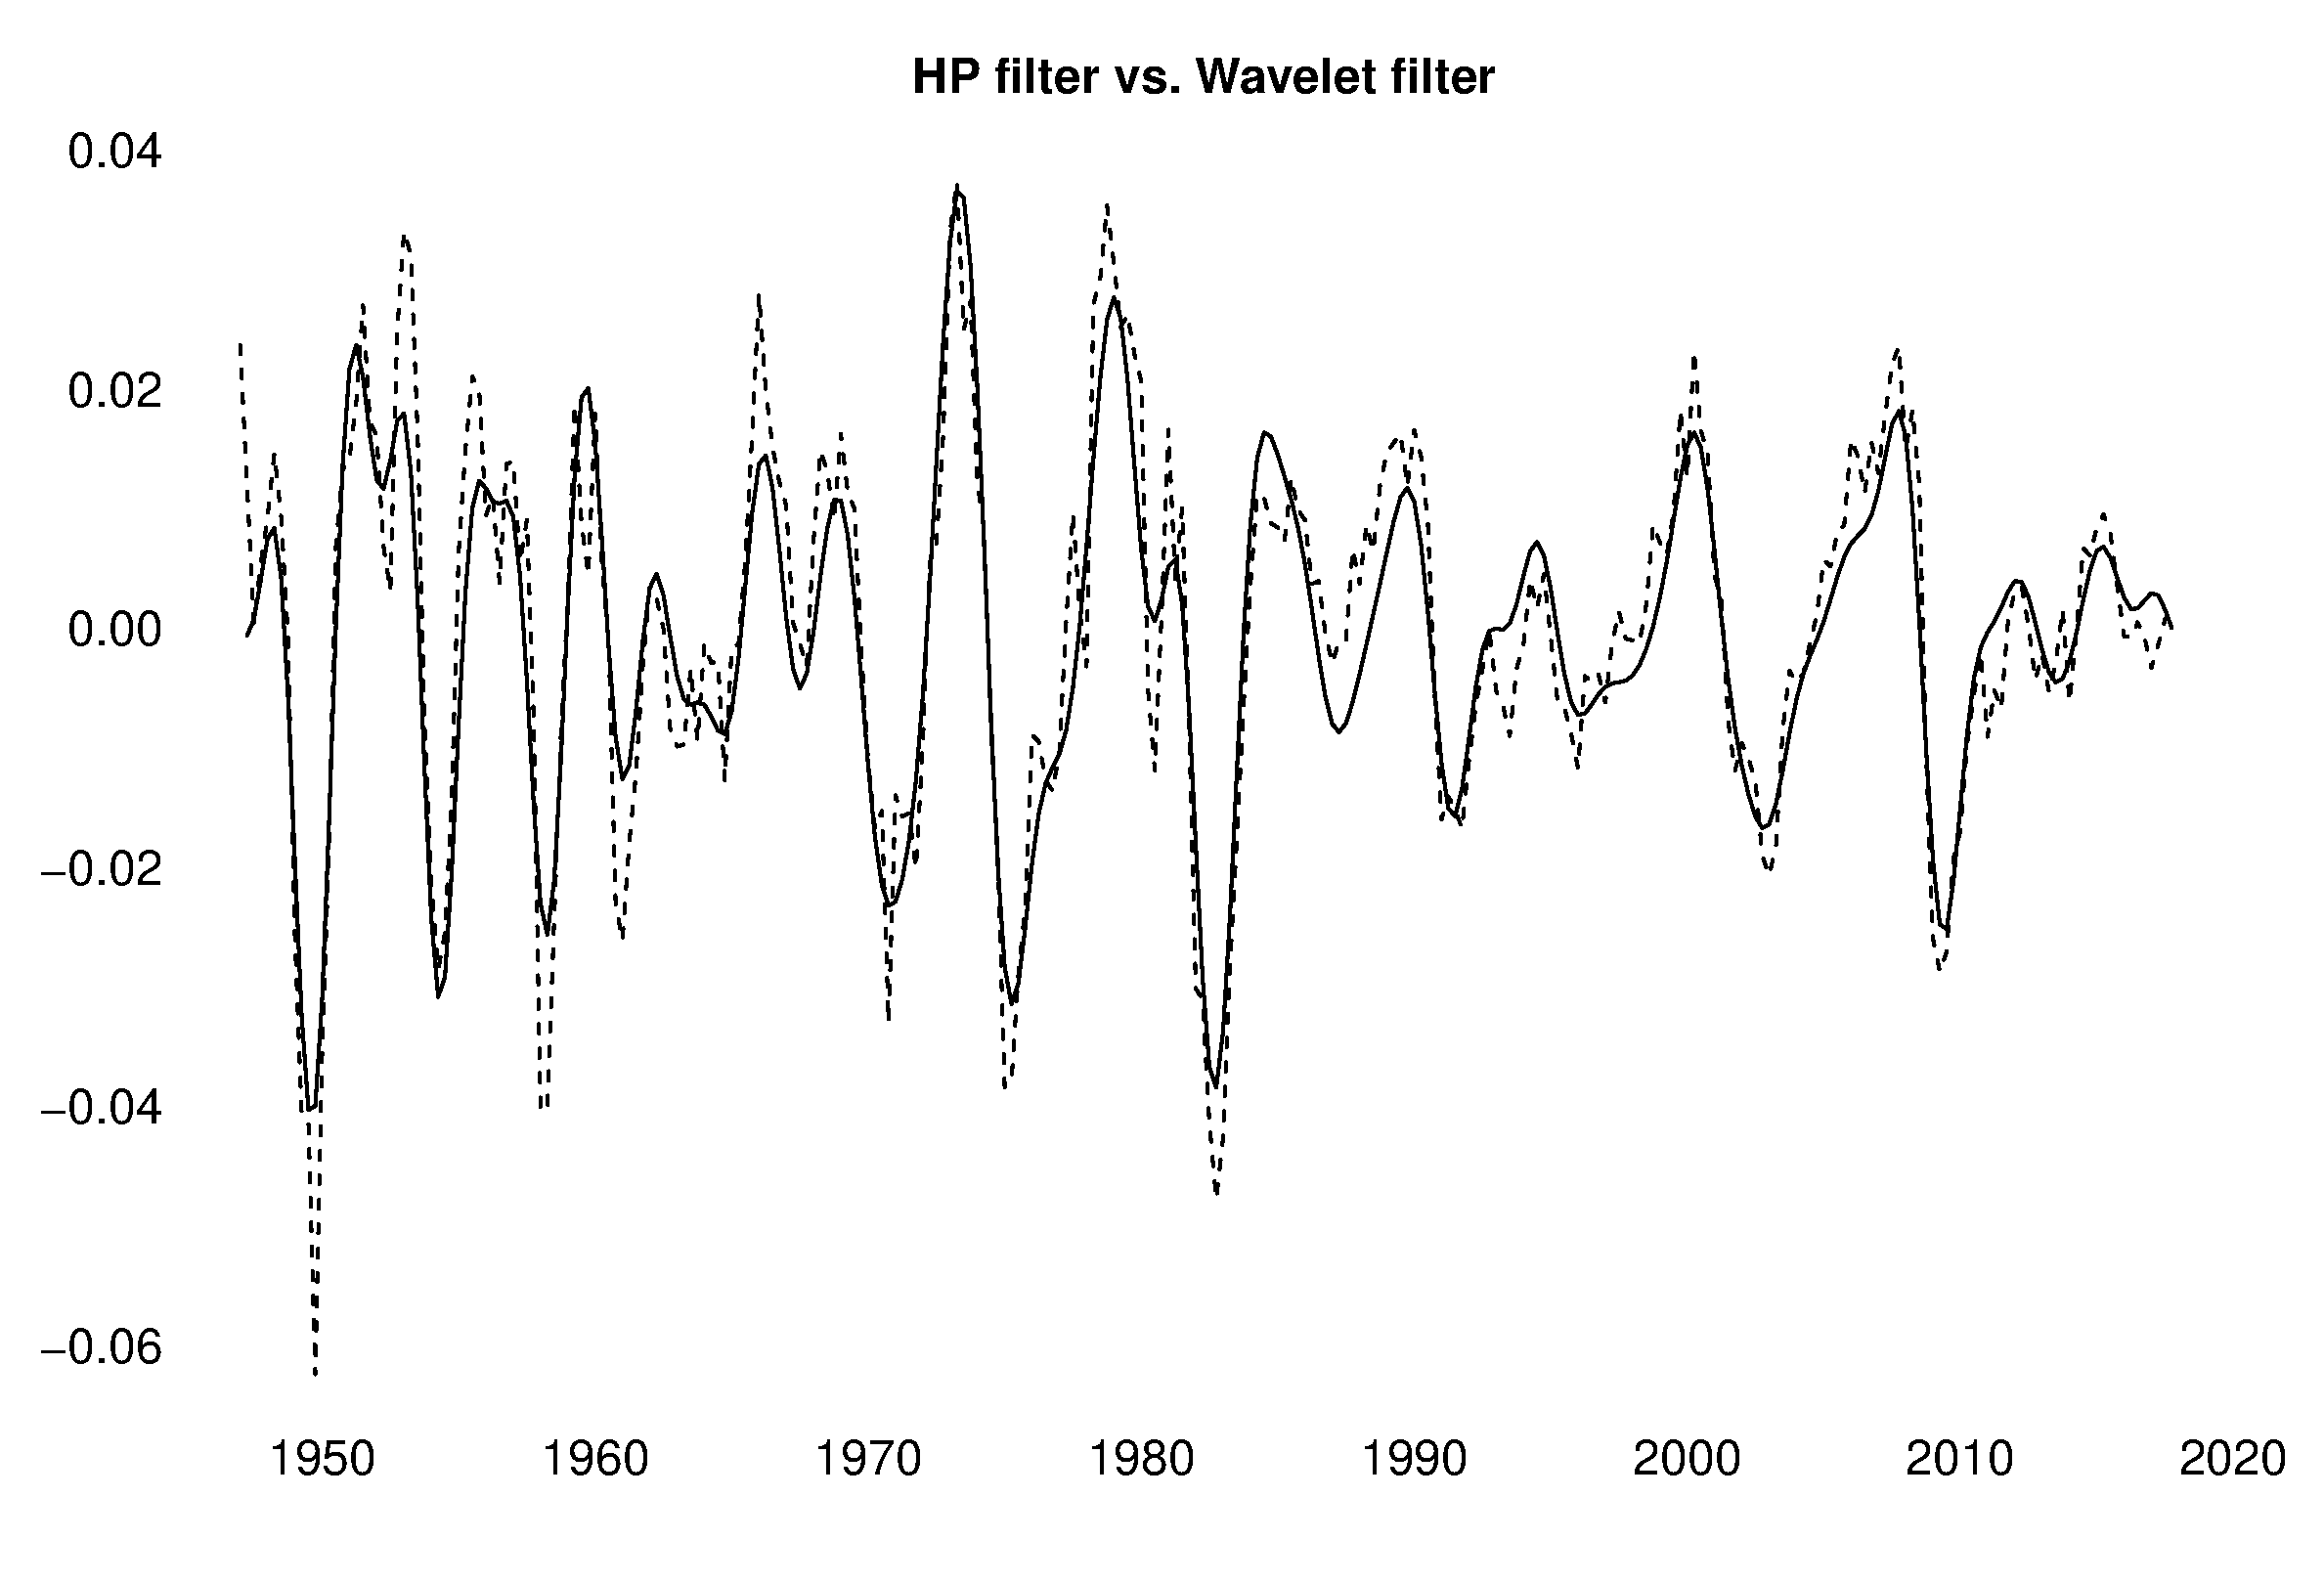
\includegraphics[scale=.3]{wavelet.eps}
  \end{figure}
\end{frame}
%--------------------------------------



%--------------------------------------
\begin{frame}
  The cyclical components in time-series data can be autocorrelated and exhibit random-looking fluctuations.
  Simple way to capture these dynamics is through an Autoregression (AR) model, e.g. AR(1)
  \begin{align}
     y_t = \rho y_{t-1} + \epsilon_t
   \end{align} 
   \medskip
   $\rho$ is propagation mechanism
   \begin{itemize}
      \item Determines at which speed a shock in $\epsilon$ fade away
    \end{itemize} 
\end{frame}
%--------------------------------------

%--------------------------------------
\begin{frame}
  Time path of $y$ after a shock in $\epsilon$ is the Impulse Response Function (IRF), i.e. $t$ follows
  \begin{align}
    \epsilon_t + 1, \epsilon_{t+1}, \epsilon_{t+2},...
  \end{align}
  Instead of 
  \begin{align}
    \epsilon_t , \epsilon_{t+1}, \epsilon_{t+2},...
  \end{align}
  \medskip
  This means there is an incremental effect in all future periods of a unit shock today.  
\end{frame}
%--------------------------------------

%--------------------------------------
\begin{frame}
  Imagine AR(1) series starting at 0 with shock $\epsilon_t = 1$ followed by 0 shocks for $t+1$.
  We get that for period $t$
  \begin{align}
    y_t = 1
  \end{align}
  \medskip
  For period $t+1$
  \begin{align}
    y_{t+1} = \rho
  \end{align}
  \medskip 
  For period $t+n$
  \begin{align}
    y_{t+n} = \rho^n
  \end{align}
\end{frame}
%--------------------------------------

%--------------------------------------
\begin{frame}
  \begin{figure}
    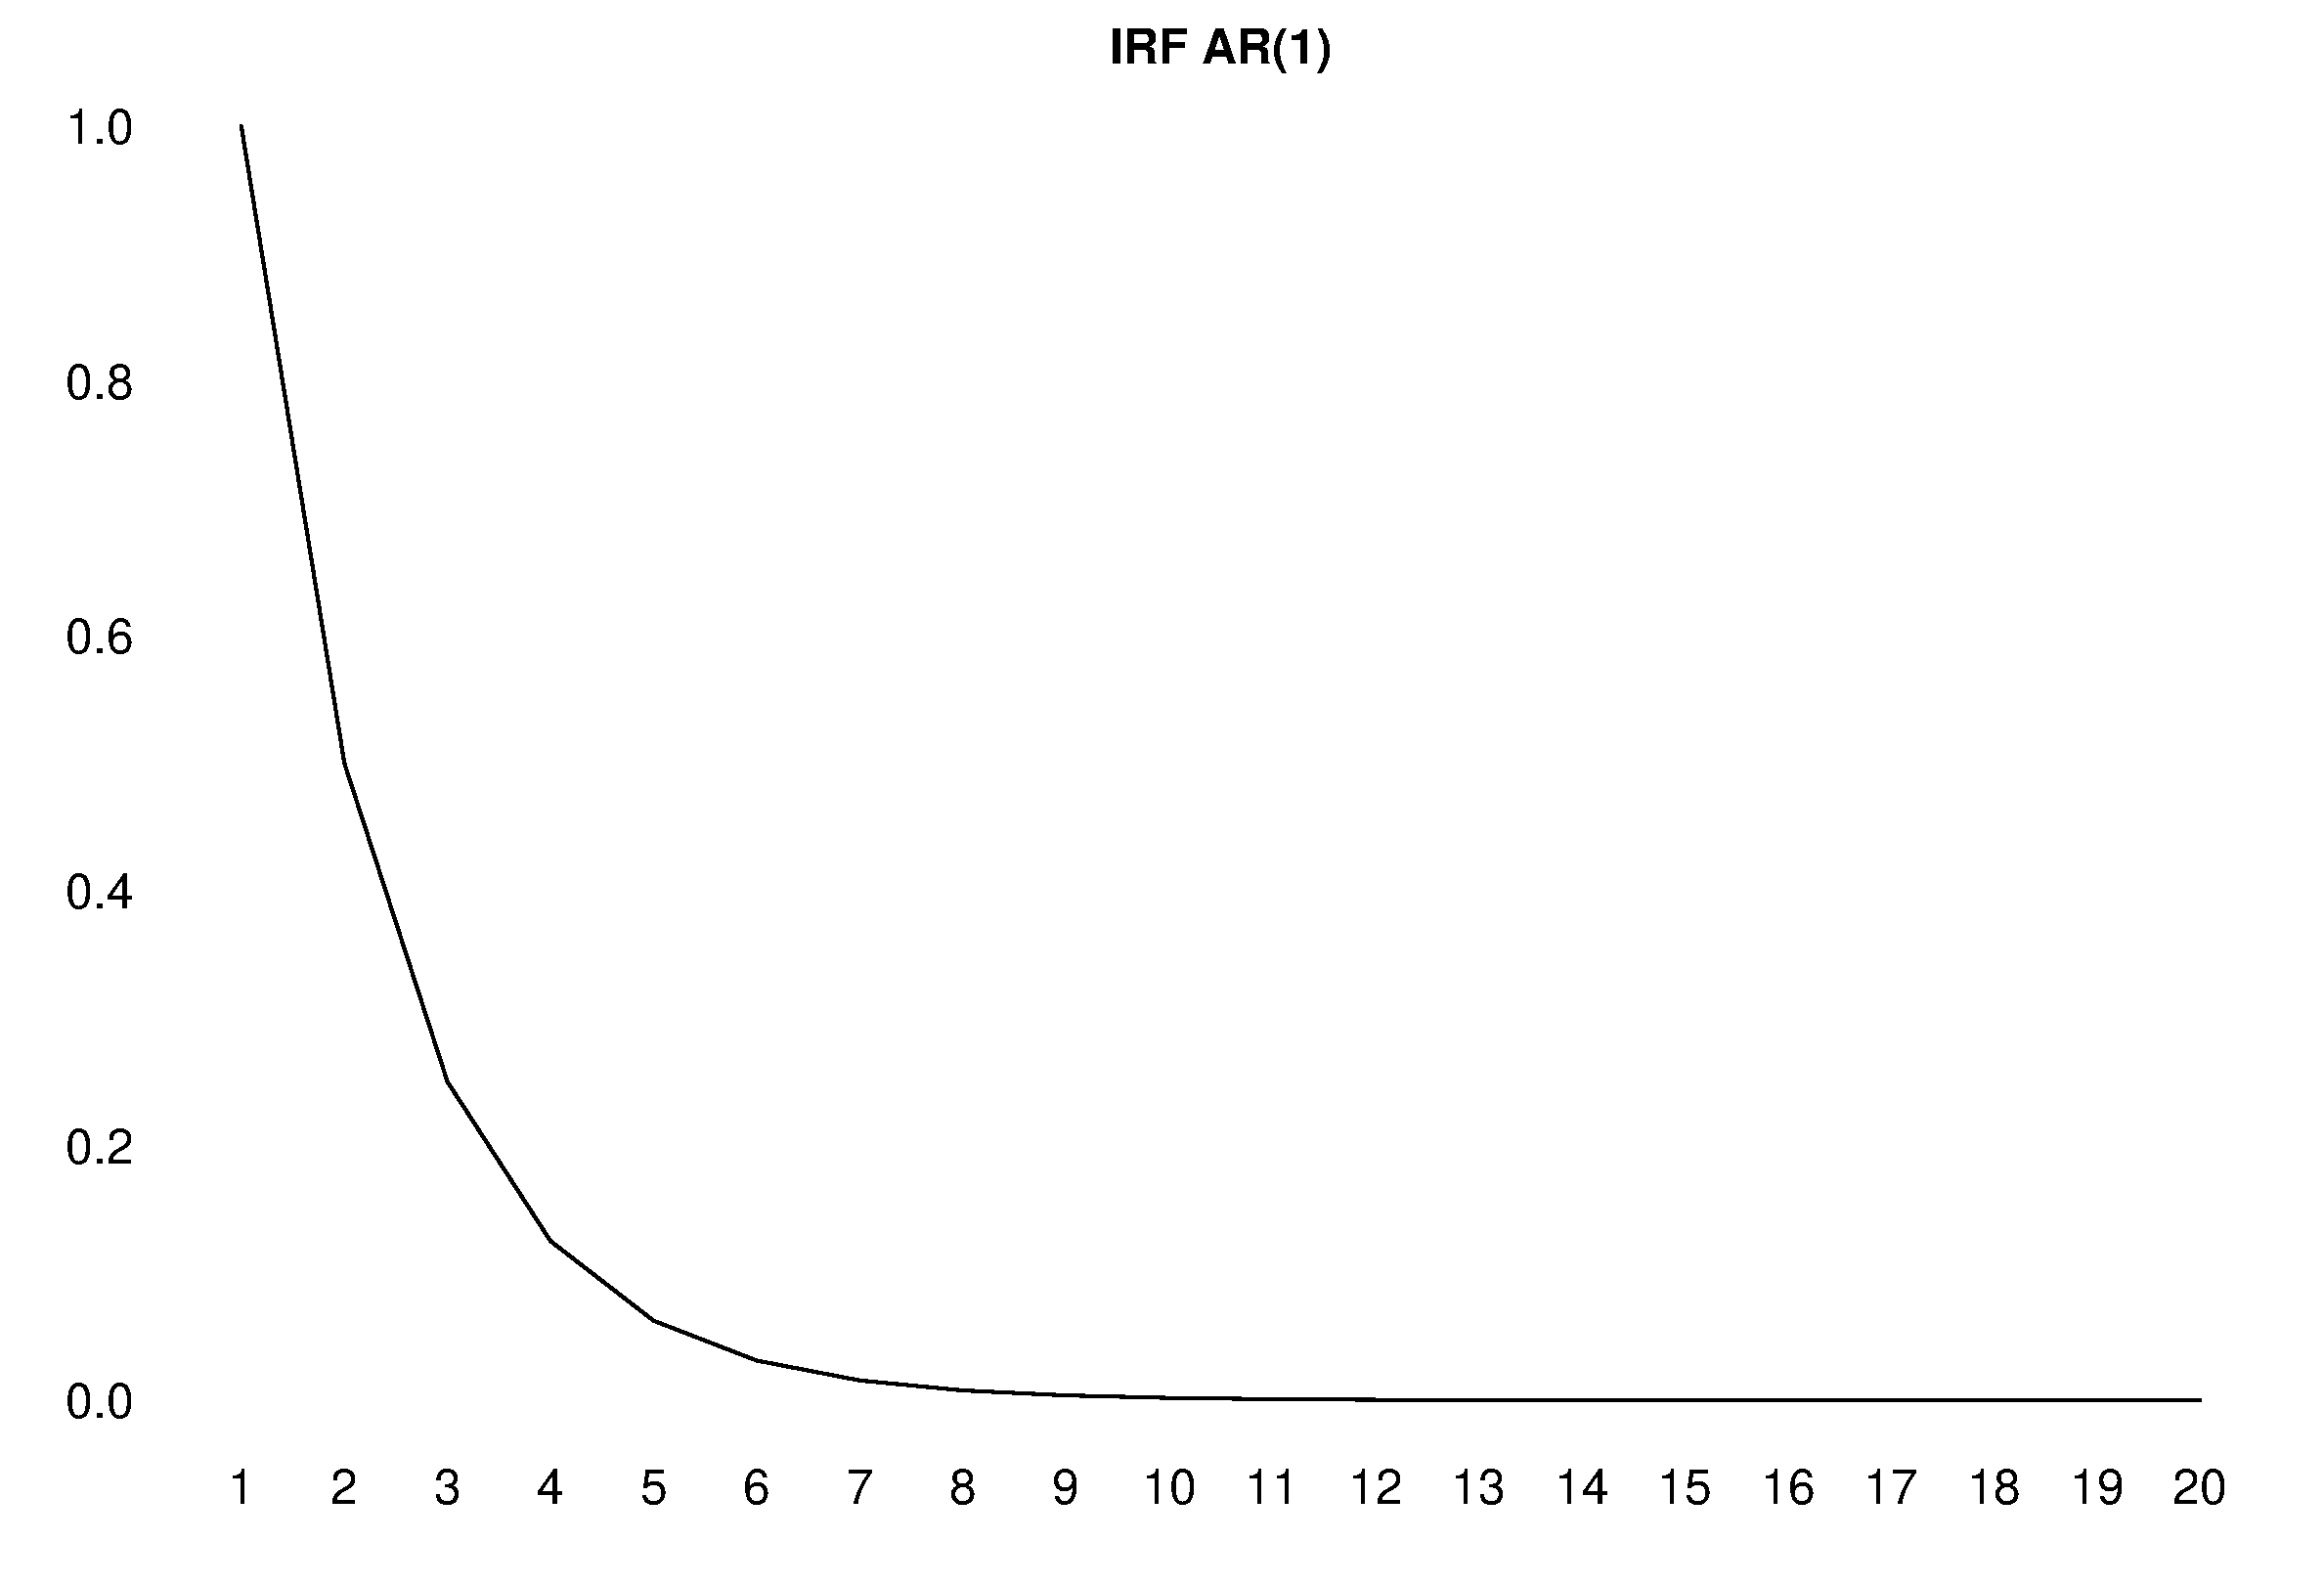
\includegraphics[scale=.3]{irf_ar1.eps}
  \end{figure}
\end{frame}
%--------------------------------------


%--------------------------------------
\begin{frame}
  Let's consider volatility which is determined by
  \begin{enumerate}
    \item Size of shock in $\epsilon$
    \item Strength of propagation mechanism $\rho$
  \end{enumerate}
  \medskip
  So for $y_t$ we get 
  \begin{align}
  \sigma_y^2 &= \rho^2 \sigma_y^2 + \sigma_\epsilon^2\\ \nonumber
  &= \frac{\sigma_\epsilon^2}{1-\rho^2}
\end{align}
\medskip
$\sigma_\epsilon^2$ is the variance of $\epsilon_t$\\
The long run variance of $y_t$ is the same as the long-run variance of $y_{t-1}$  
\end{frame}
%--------------------------------------

%--------------------------------------
\begin{frame}
  \begin{figure}
    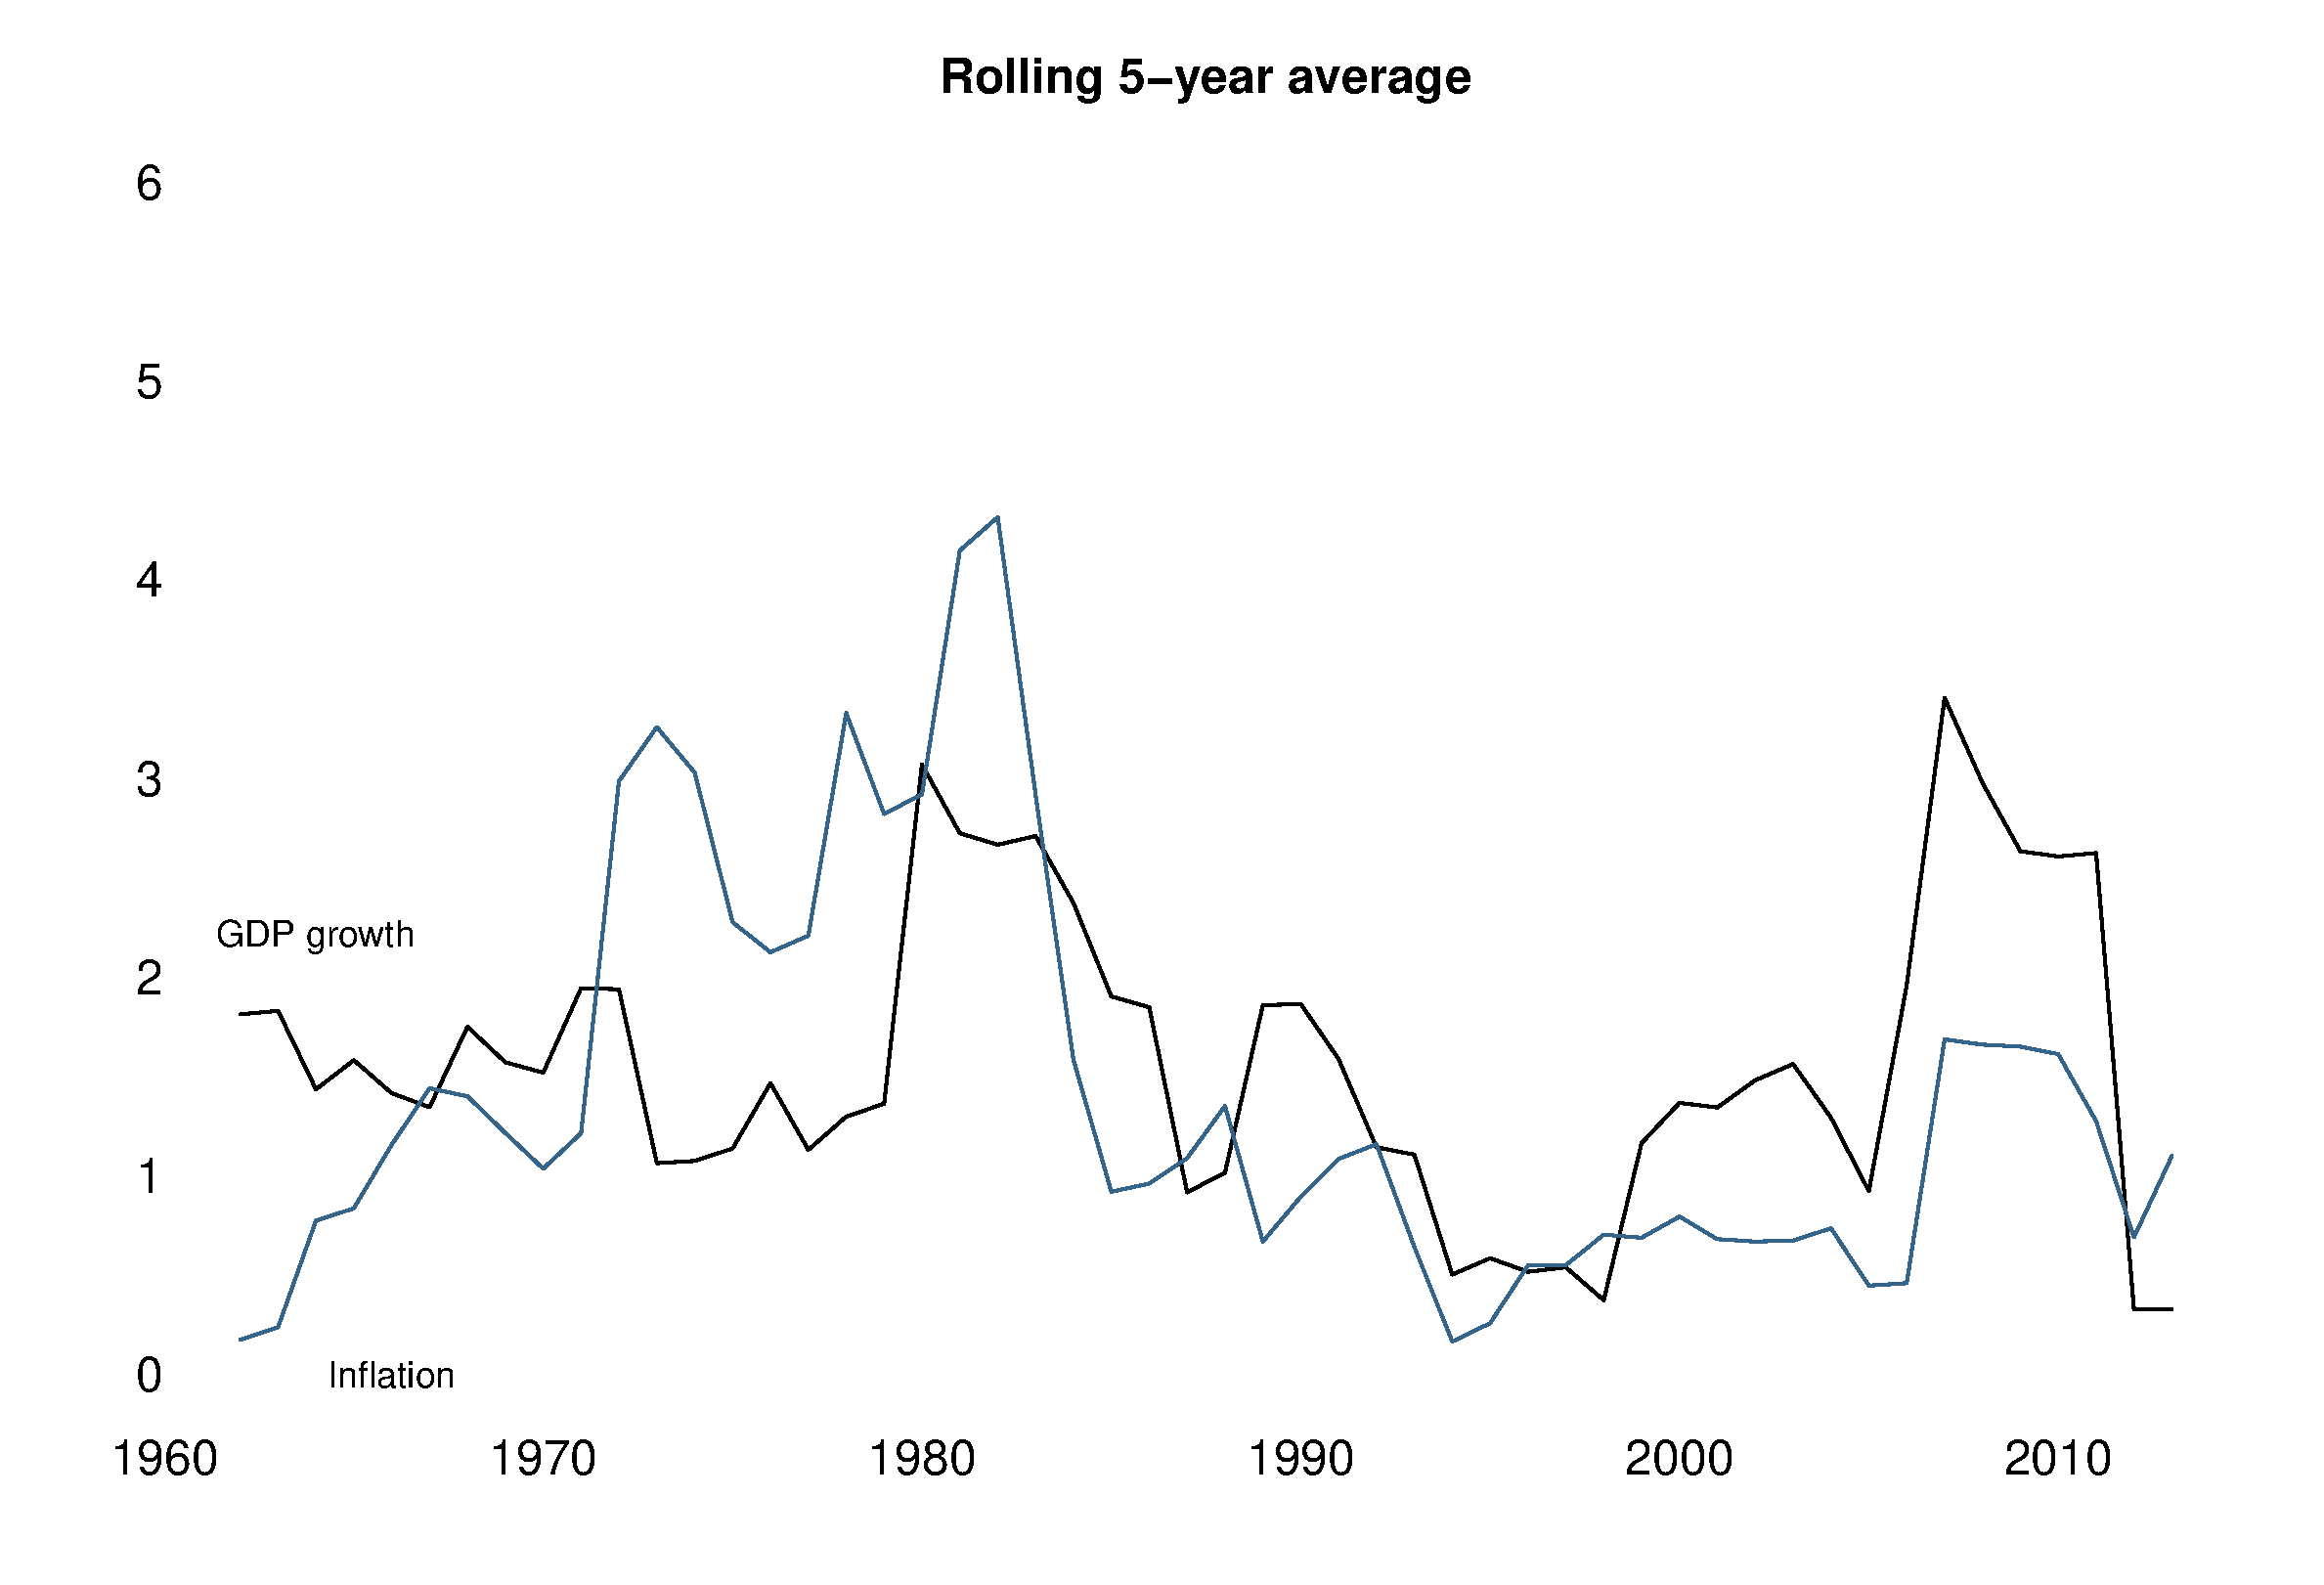
\includegraphics[scale=.3]{great_moderation.eps}
  \end{figure}
\end{frame}
%--------------------------------------

%--------------------------------------
\begin{frame}
  \textbf{the Great Moderation:} Since mid-1980s output and inflation have become less volatile, which could be due to
  \begin{enumerate}
  \item Smaller shocks (lower values for $\epsilon_t$)
  \begin{itemize}
    \item Less random policy shocks
    \item Smaller shocks from goods and/or financial markets
    \item Smaller supply shocks
  \end{itemize}
  \medskip
  \item Weaker propagation mechanisms (lower values for $\rho$)
  \begin{itemize}
    \item Policy became more stabilizing
    \item More stable economy
    \item Stabilisation of economy due to financial modernisation
  \end{itemize}
\end{enumerate}
\end{frame}
%--------------------------------------

%--------------------------------------
\begin{frame}
  \textbf{Slutsky effect:} when data are uncorrelated smoothing can introduce appearance of irregular oscillations (Kelly \& O'Grada, 2014).
  There are two different definitions, the formal one
  \begin{align}
     f(\omega)=\frac{1}{m^2} \frac{1-cos\;m\omega}{1-cos\;\omega}     
   \end{align} 
   \medskip
   This is the transfer function for a moving average of $m$ periods.
   And there is the colloquial one
   \begin{quote}
     Applying a moving average to a white noise series will generate the appearance of irregular oscillations, as the filter is distorted by runs of high or low observations.
   \end{quote}
\end{frame}
%--------------------------------------


%--------------------------------------
\begin{frame}
  \begin{figure}
    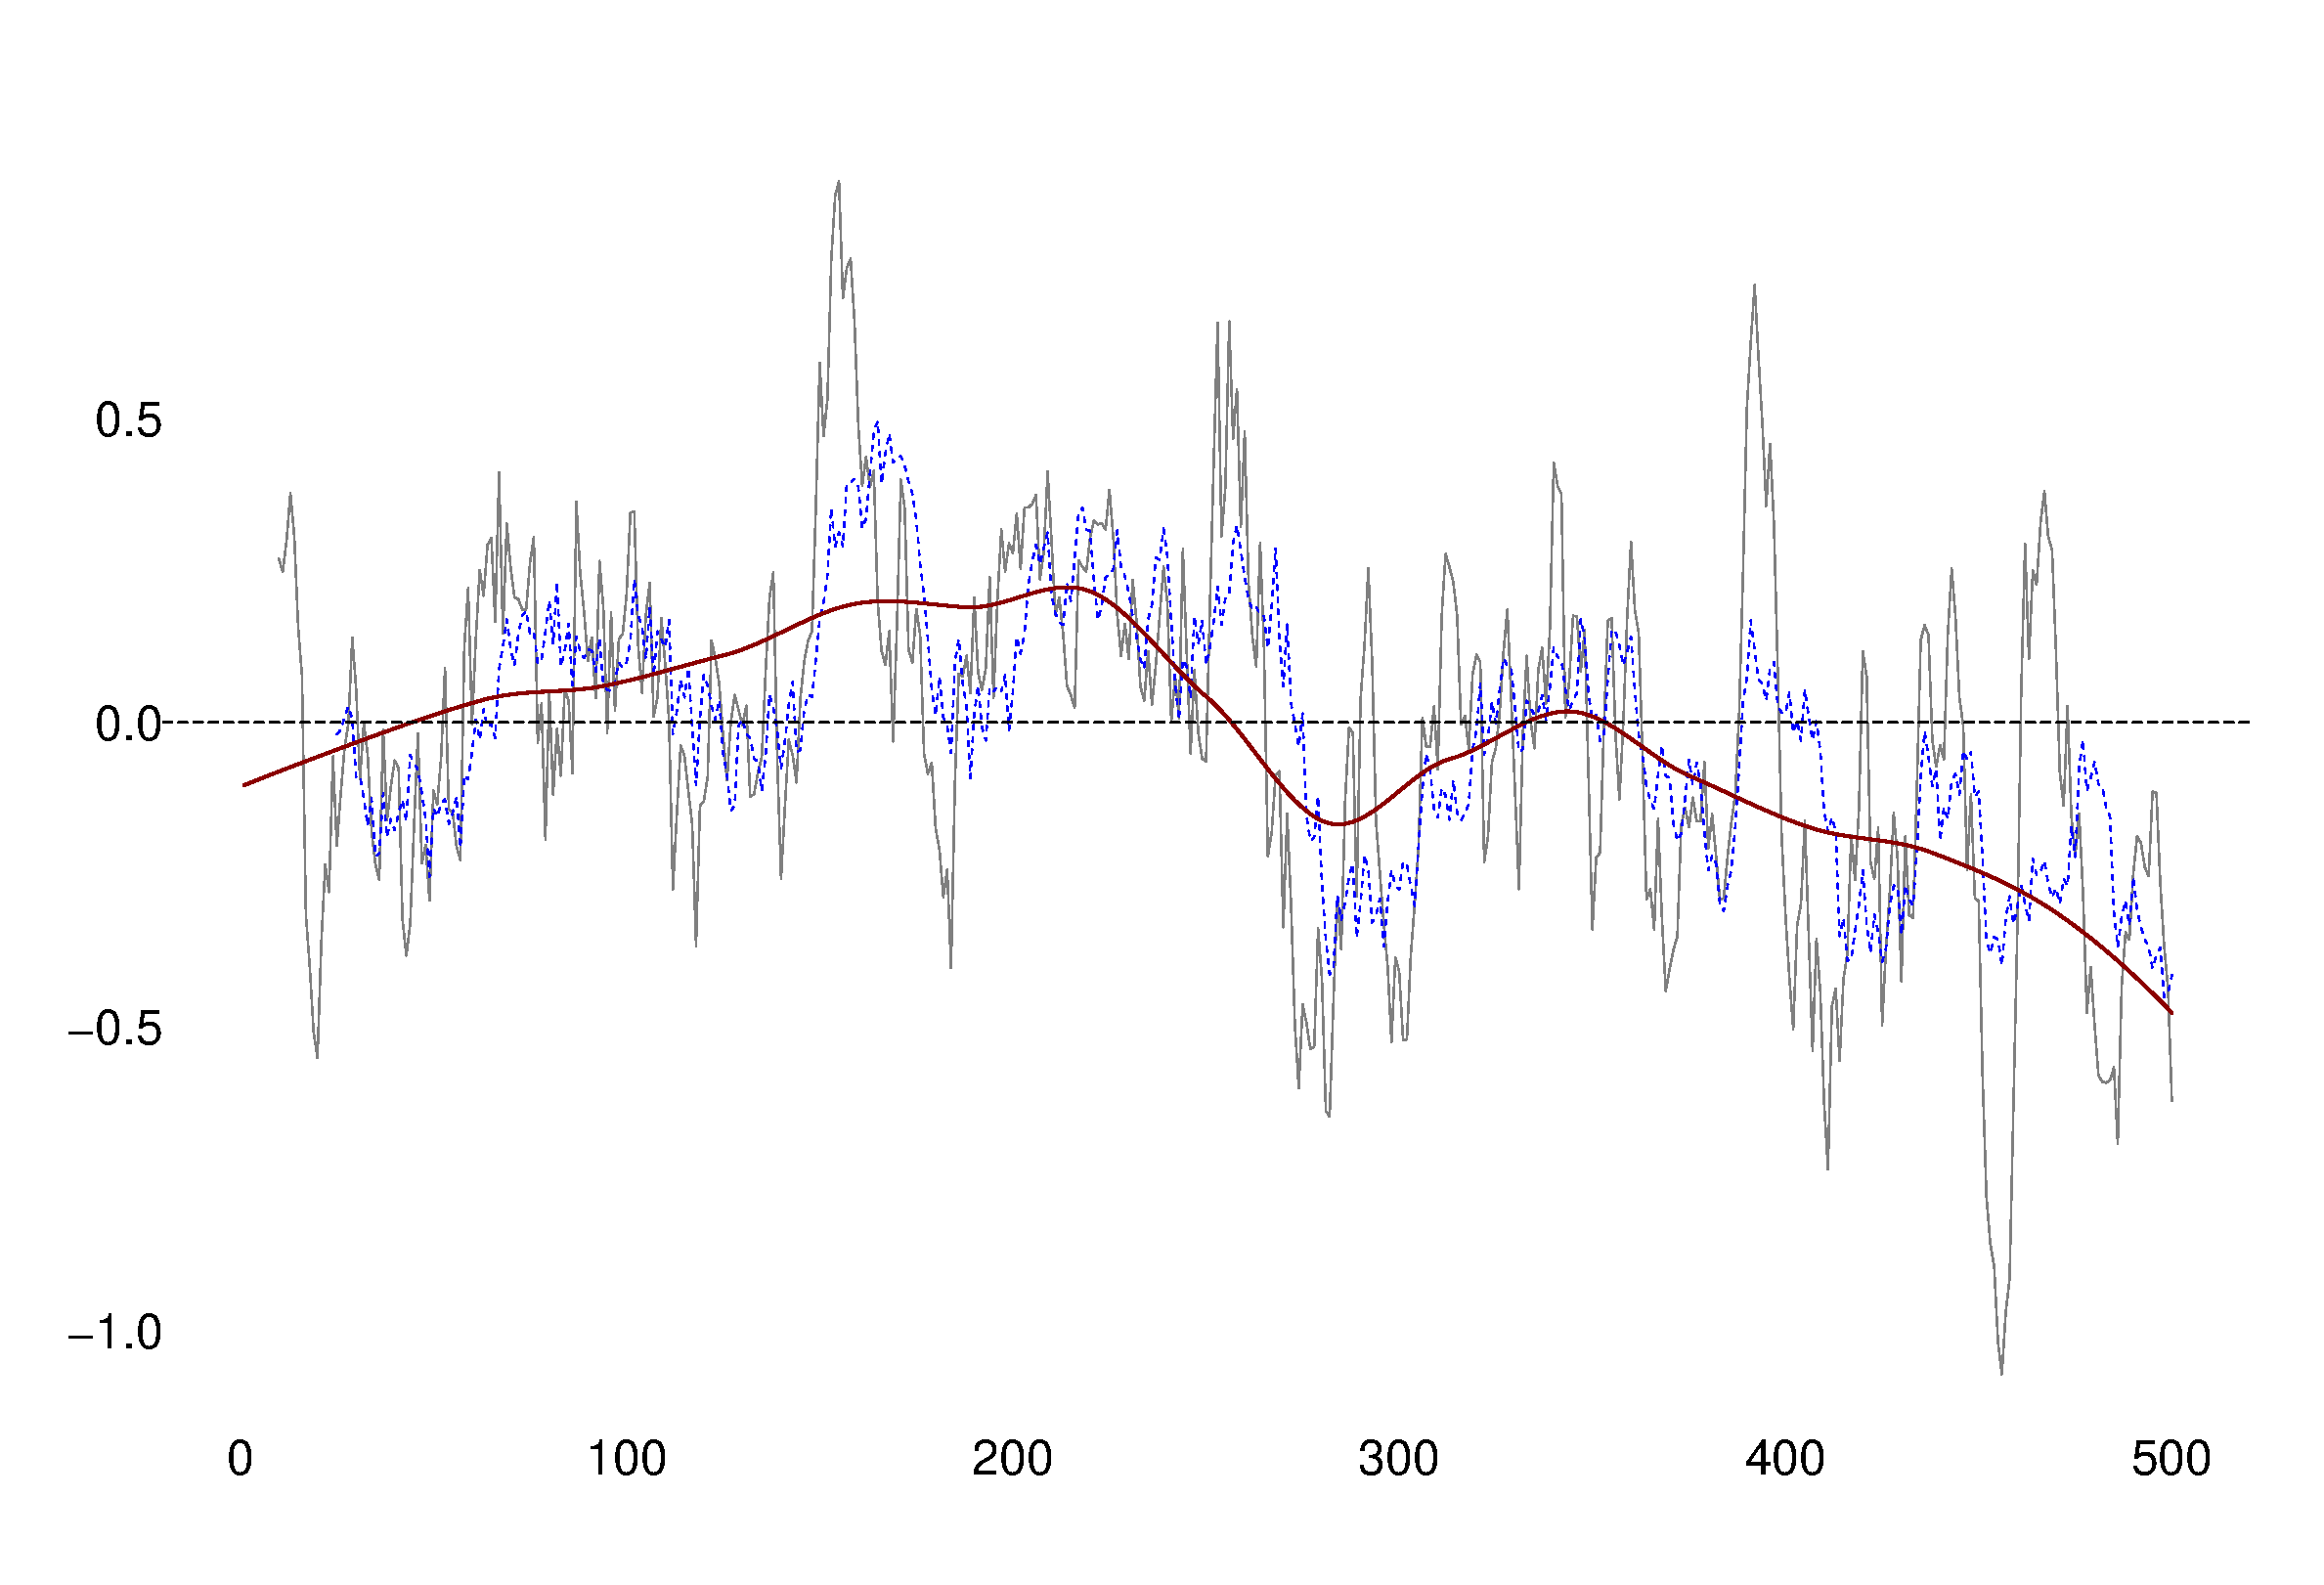
\includegraphics[scale=.3]{slutsky.eps}
  \end{figure}
\end{frame}
%--------------------------------------

%--------------------------------------
\begin{frame}
  \begin{figure}
    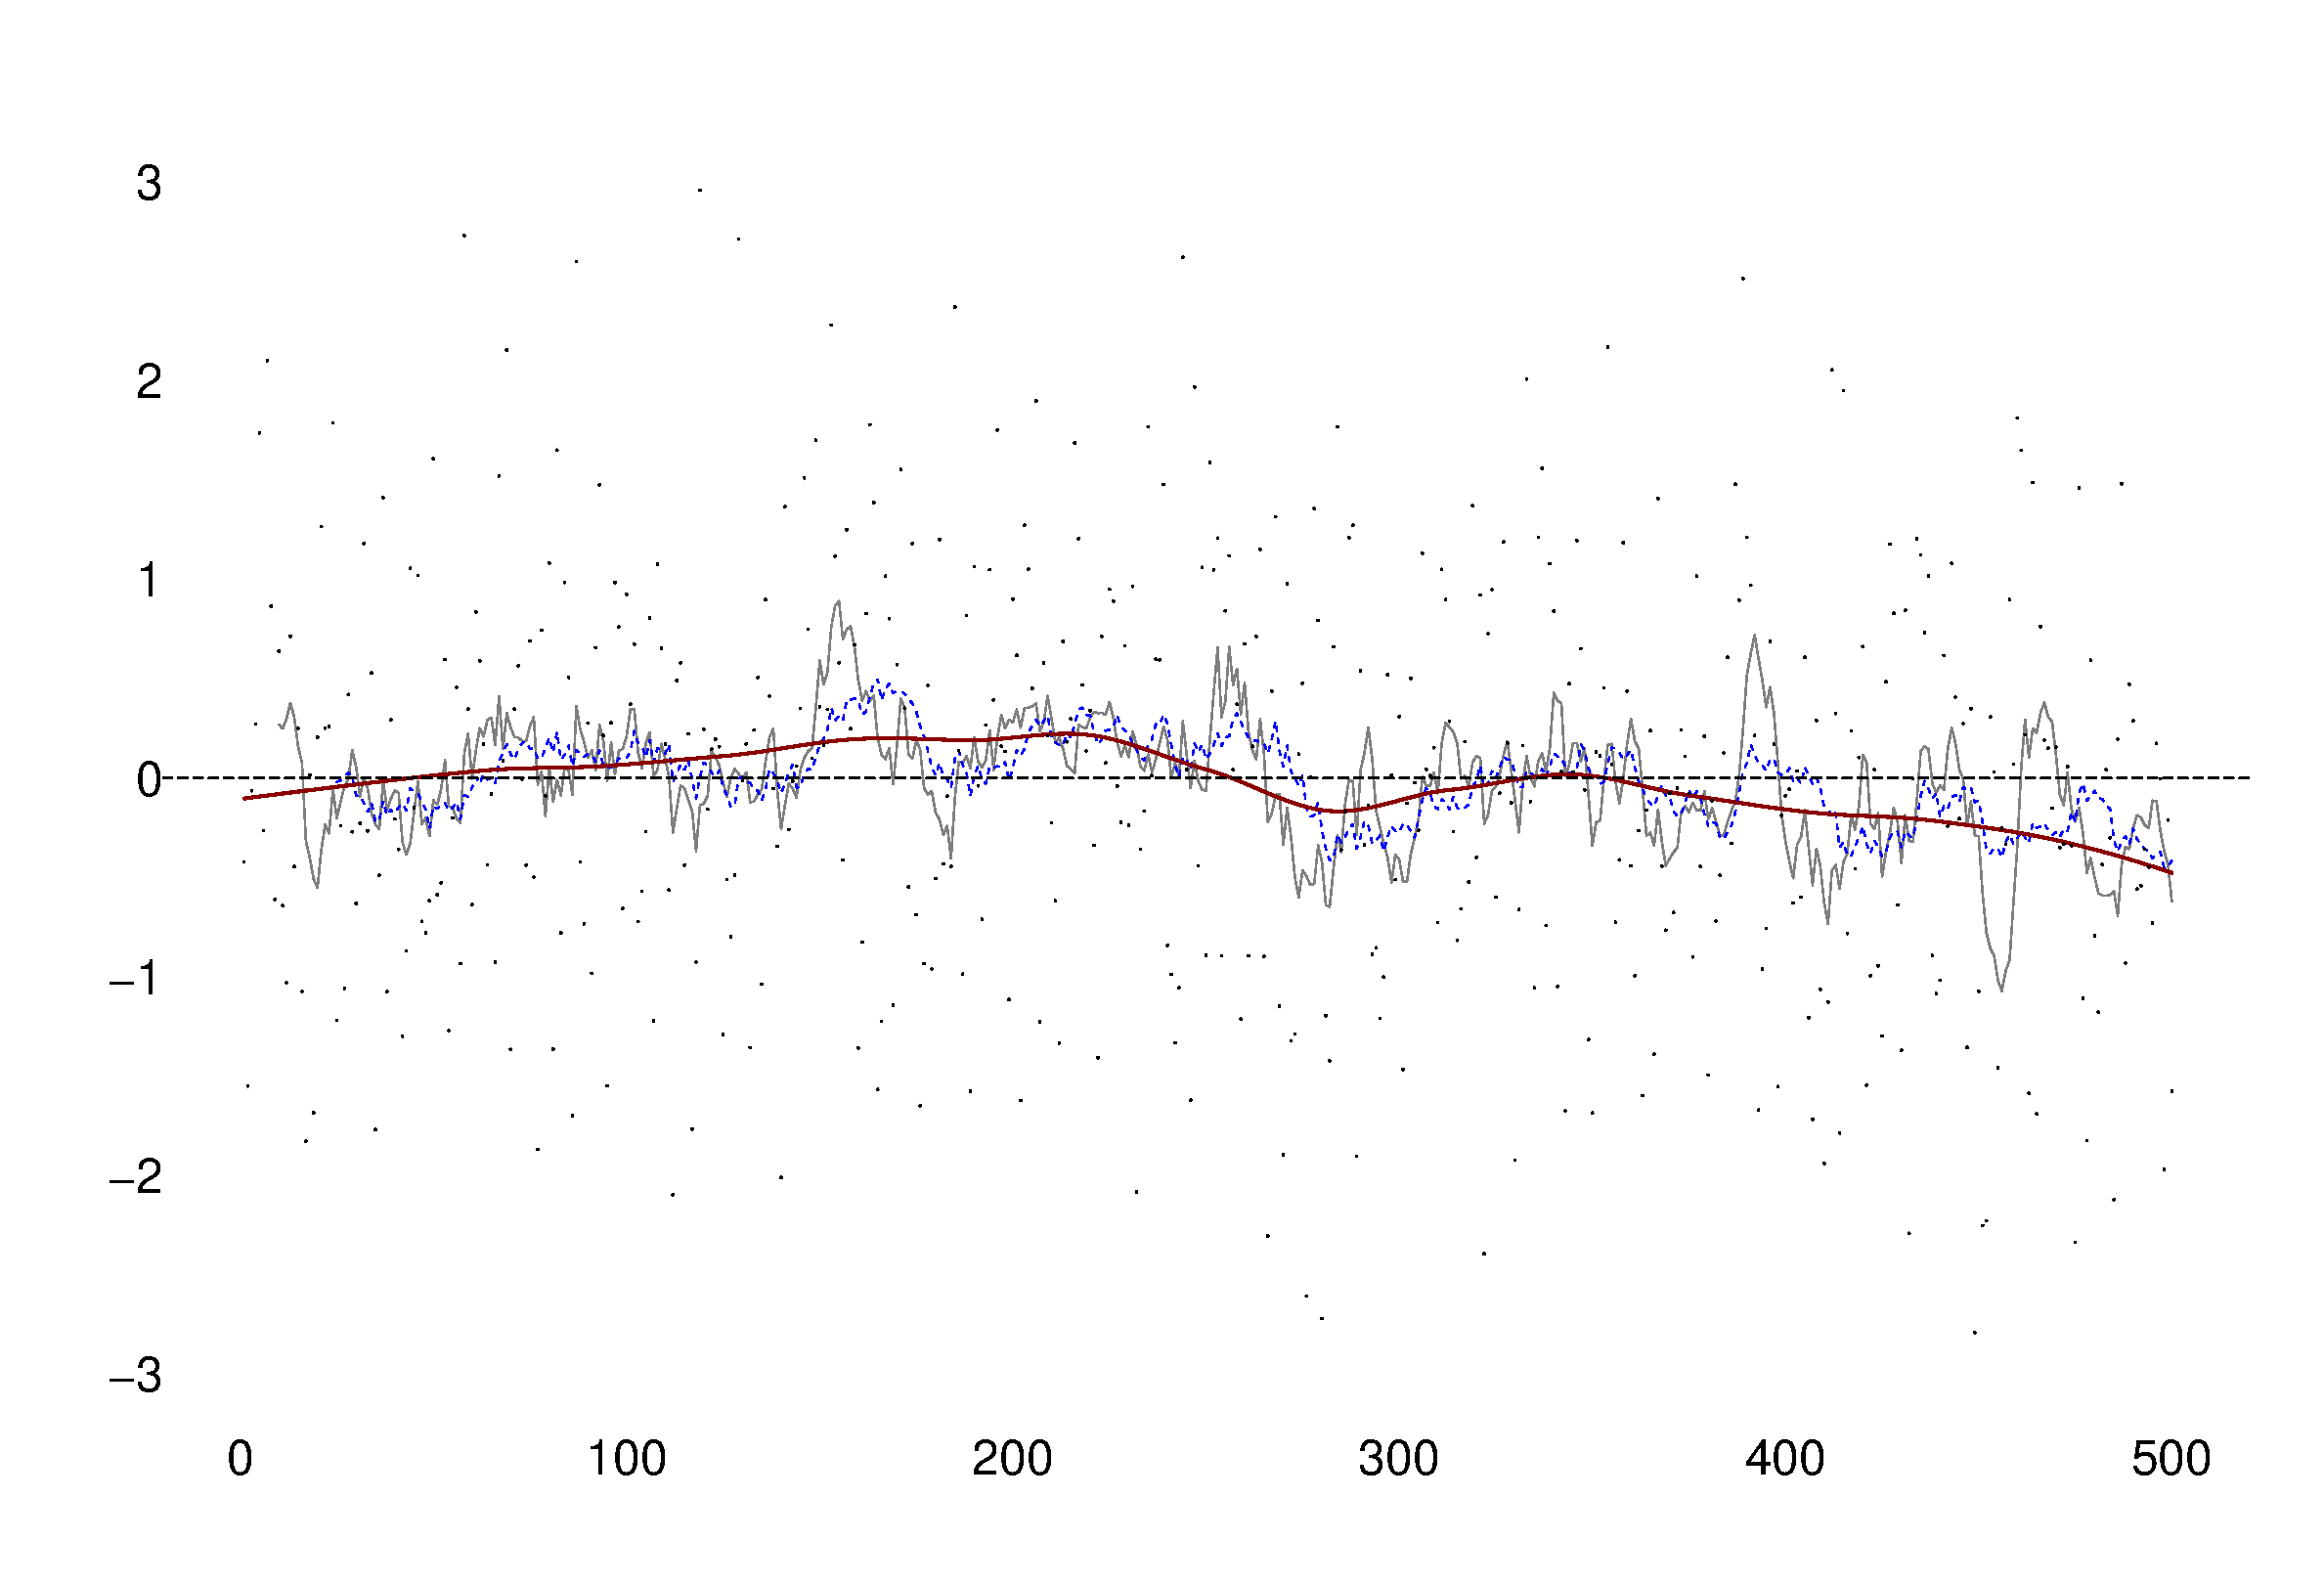
\includegraphics[scale=.3]{slutsky2.eps}
  \end{figure}
\end{frame}
%--------------------------------------


%--------------------------------------
\begin{frame}
  Often macroeconomic dynamics extend beyond AR(1) process; consider AR(2) model
  \begin{align}
  y_t = \alpha + \rho_1 y_{t-1} + \rho_2 y_{t-2} + \epsilon_t
  \end{align}
  \medskip
  IRF can take on various forms based on $\rho_1,\rho_2$ values
  \begin{itemize}
    \item More complex responses can be generate by AR(p) model
    \item Dynamic properties of model depend on number of lags $p$ included in model
  \end{itemize}
\end{frame}
%--------------------------------------

%--------------------------------------
\begin{frame}
  \begin{figure}
    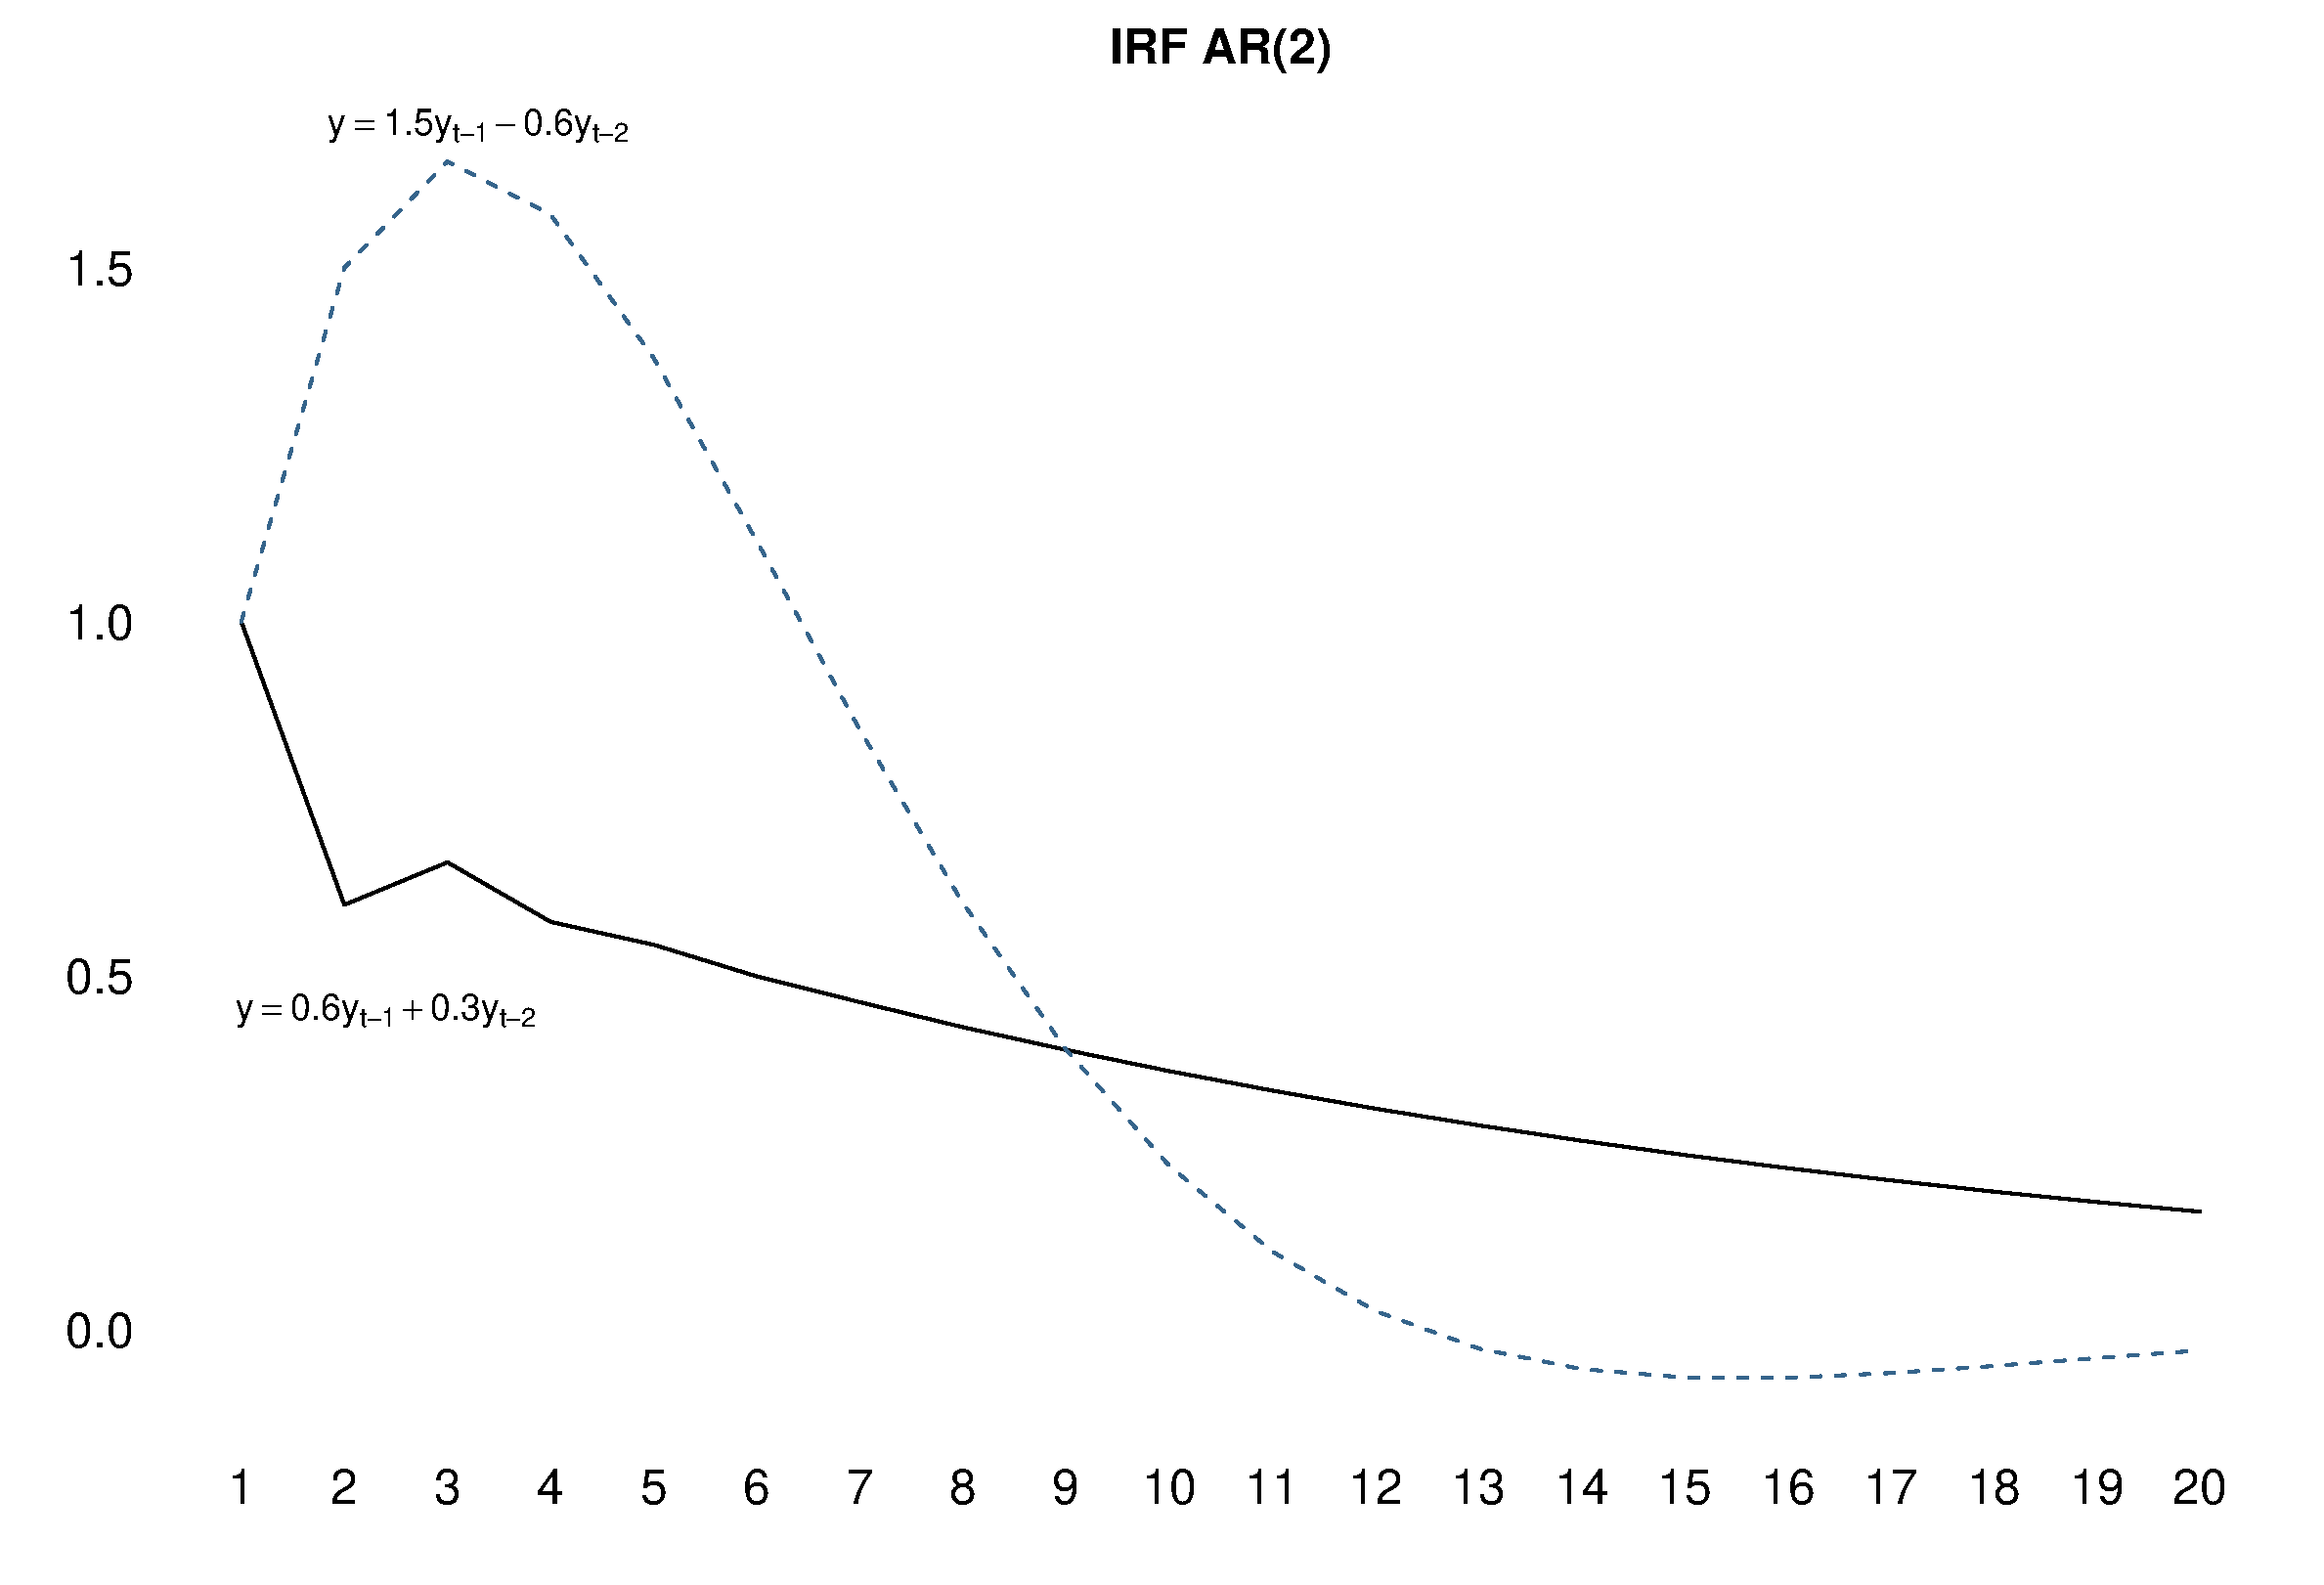
\includegraphics[scale=.3]{irf_ar2.eps}
  \end{figure}
\end{frame}
%--------------------------------------

%--------------------------------------
\begin{frame}
  \begin{figure}
    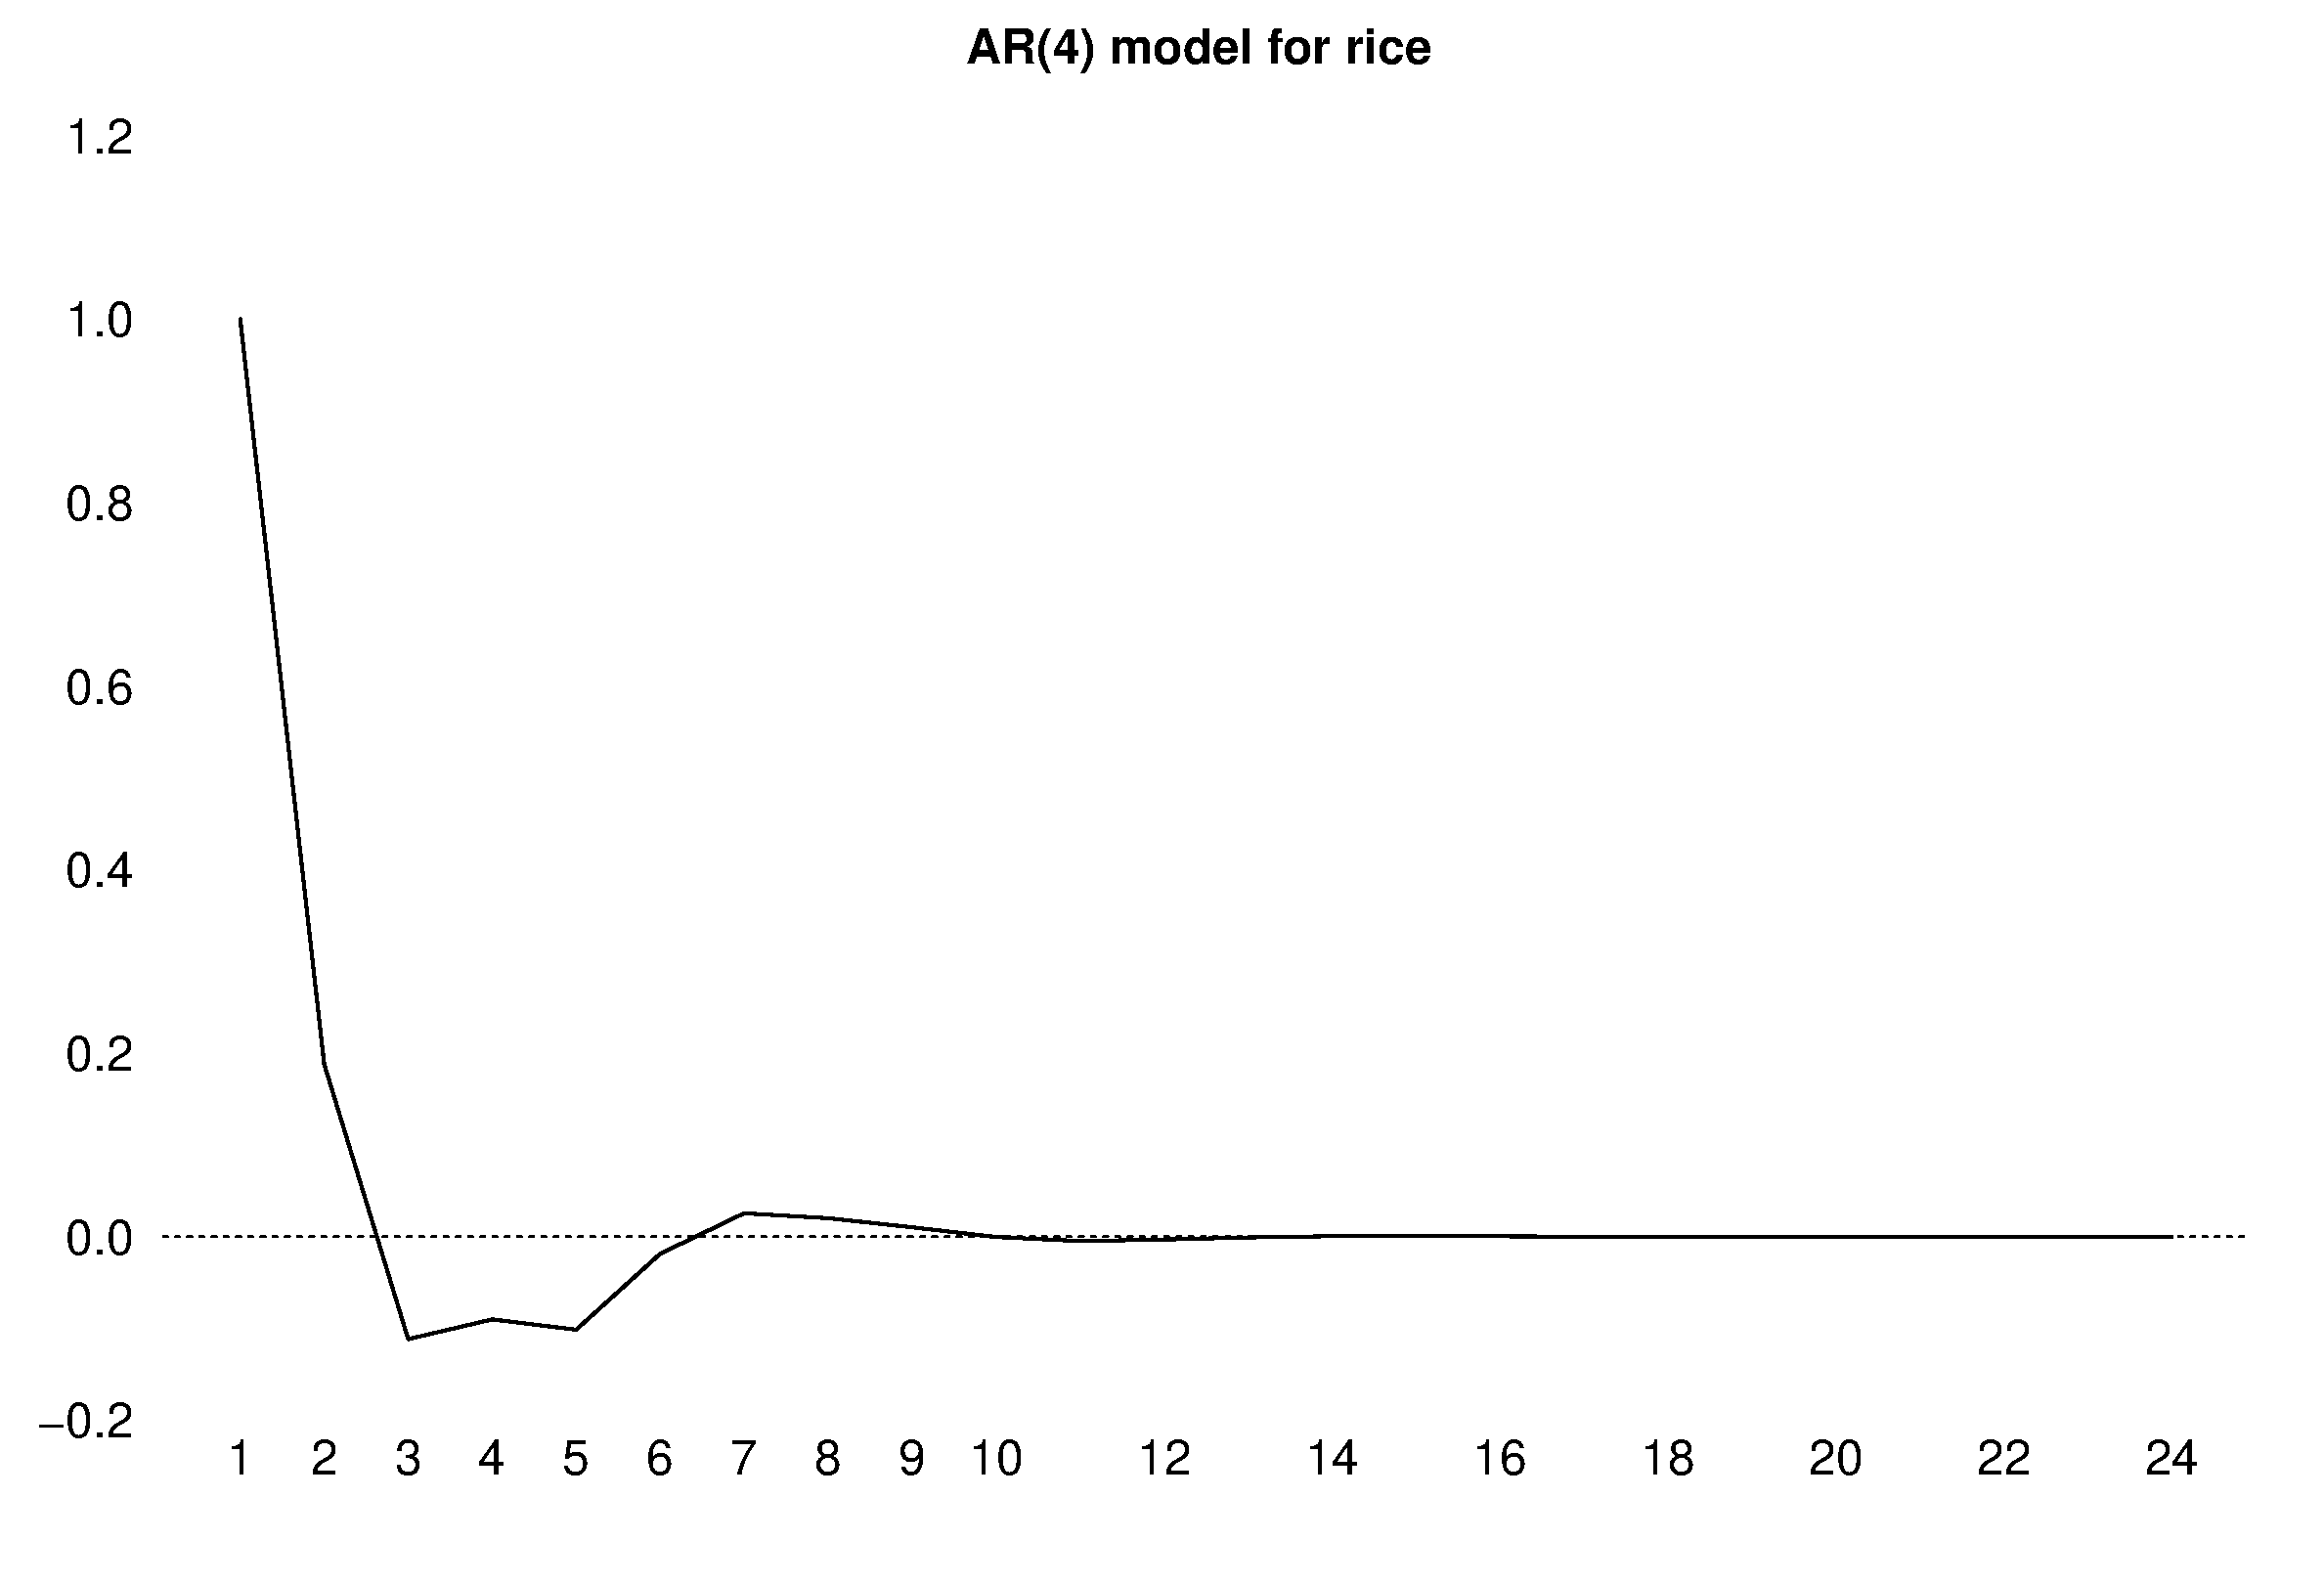
\includegraphics[scale=.3]{rice4.eps}
  \end{figure}
\end{frame}
%--------------------------------------

%--------------------------------------
\begin{frame}
  Concerning model notation; we can use the lag operator $L$
  \begin{itemize}
    \item The operator moves the time-series back in time
  \end{itemize}
  So instead of 
  \begin{align}
      y_{t-1}
    \end{align}
    \medskip
    We can write
    \begin{align}
        Ly_t
      \end{align}
    \medskip
    Similarly
    \begin{align}
       L^2y_t &= y_{t-2}
      \end{align}  
\end{frame}
%--------------------------------------

%--------------------------------------
\begin{frame}
 Can use the lag operator in model specification when the model includes a number of lags.
 Can write model 
  \begin{align}
    y_t = a_1 y_{t-1} + a_2 y_{t-2} + \epsilon_t
  \end{align}
  \medskip
  as
  \begin{align}
    y_t = A(L)y_t + \epsilon_t, \; A(L) = a_1 L + a_2 L^2
  \end{align}
  \medskip
  Alternatively you can write it as
  \begin{align}
    B(L)y_t = \epsilon_t,\; B(L) = 1-a_1 L + a_2 L^2
  \end{align}  
\end{frame}
%--------------------------------------

%--------------------------------------
\begin{frame}
  $AR$ models are useful in understanding the dynamics of individual variables
  \begin{itemize}
    \item But they ignore the relationships between variables
  \end{itemize}
  Vector Autoregressions ($VAR$) model the dynamics between $n$ different variables, allowing each variable to depend on the lagged values of all the variables
  \begin{itemize}
    \item Can examine the impulse response of $n$ variables to all $n$ shocks
  \end{itemize}
  \medskip
  Simplest VAR model has two variables and one lag
  \begin{align}
    y_{1t} &= a_11 y_{1, t-1} + a_12 y_{2,t-1} + \epsilon_{1t}\\
    y_{2t} &= a_21 y_{1, t-1} + a_22 y_{2,t-1} + \epsilon_{2t}
  \end{align}
\end{frame}
%--------------------------------------


%--------------------------------------
\begin{frame}
  Lot of talk about shocks: some sources include
  \begin{enumerate}
    \item Policy changes, which are not captured by the systematic component of the VAR equation
    \item Changes in preferences, such as work vs. leisure or spending vs. saving
    \item Technology shocks, which are random changes in the productivity of firms
    \item Shocks to various frictions, like changes in the efficiency with which markets (labour, goods, financial) work
  \end{enumerate}
\end{frame}
%--------------------------------------

%--------------------------------------
\begin{frame}
 Time-series perspective is central to economic fluctuations in macroeconomics
 \begin{itemize}
   \item Cycles are determined by various random shocks, propagated throughout the economy over time
 \end{itemize}
 \medskip
 VARs are commonly used for modeling macroeconomic dynamics and the effect of shocks
 \begin{itemize}
   \item Can help explain \textit{how} things work, but not \text{why} things work the way they do   
 \end{itemize}
 \medskip
 Dynamics Stochastic General Equilibrium model build upon VAR framework, but dynamics are derived from economic theory
 \begin{itemize}
   \item In this framework agents are i) rational and ii) optimising
 \end{itemize}
\end{frame}
%--------------------------------------








%--------------------------------------
\end{document}
